%
%   SAC参考手册
%   作者:SeisMan
%   项目主页:https://github.com/seisman/SAC_Docs_zh
%   文档发布页:http://seisman.info/sac-manual.html
%   编译环境:TeXLive 2014
%   中文支持:xeCJK + xeLaTeX
%

\documentclass[a4paper, 11pt, twoside]{book}
%
% LaTeX配置文件
%

% 文档相关信息
\newcommand{\SACDOCTITLE}{SAC\textbf{参考手册}} % 文档标题
\newcommand{\SACDOCAUTHOR}{SeisMan}             % 文档作者
\newcommand{\SACDOCVERSION}{3.2-dev}                % 文档版本
\newcommand{\SACDOCDATE}{\today}                % 文档更新日期

% SAC相关信息
\newcommand{\SACVERSION}{101.6a}                % 文档对应的SAC版本
\newcommand{\SACDATE}{2013-11-11}               % SAC的发布日期

% 中文支持及中英文字体设置
\usepackage[
    indentfirst,    % 章节标题后首段缩进
    CheckSingle,    % 避免单个CJK字符位于段落最后一行
]{xeCJK}

% 页面设置
\usepackage[top=3.0cm,bottom=2.0cm,left=3.5cm,right=2.5cm]{geometry}

% 间距设置
\usepackage{indentfirst}
\linespread{1.3}                        % 行间距
\addtolength{\parskip}{3pt}             % 段落间距
\setlength{\parindent}{2em}             % 首行缩进

% 标题设置
\usepackage{titlesec}
% 设置Part格式
\titleformat{\part}{\centering\Huge\bfseries}{第\,\thepart\,部分}{1em}{}
% 设置章格式
\titleformat{\chapter}{\centering\Huge\bfseries}{第\,\thechapter\,章}{1em}{}
% 调整subsection前后间距
\titlespacing*{\subsection}{0ex}{-.2ex}{.2ex}
\titlespacing*{\subsubsection}{0ex}{-.1ex}{.1ex}
%设置SACTitle为subsection格式
\newcommand{\SACTitle}[1]{\subsection*{#1}}
\newcommand{\SACCMD}[1]{\section{\texttt{#1}}}

% 目录设置
\usepackage{titletoc}
\setcounter{tocdepth}{2}
\titlecontents{chapter}[0em]
{\vspace{0.2em}\bfseries\Large}
{\thecontentslabel\quad}
{\hspace*{0em}}
{\hfill \contentspage}
\titlecontents{section}[1em]
{\large}
{\thecontentslabel\quad}
{\hspace*{0em}}
{\ \dotfill \ \contentspage}
[\vspace{-0.3em}]

\titlecontents{subsection}[3em]
{\normalsize}
{\thecontentslabel\quad}
{\hspace*{0em}}
{\ \dotfill \ \contentspage}
[\vspace{-0.3em}]

% 双栏目录
\usepackage{multicol}
\makeatletter
\renewcommand{\tableofcontents}{%
\setlength{\columnsep}{2.5em}
\begin{multicols}{2}[\chapter*{\contentsname}]%
    \@starttoc{toc}%
\end{multicols}}
\makeatother

% 页眉页脚设置
\usepackage{titleps}
\newpagestyle{body}{
    \sethead
    [$\cdot$~\thepage~$\cdot$][][\small\S\,\thesection\quad\sectiontitle]
    {第\,\thechapter\,章\quad\chaptertitle}{}{$\cdot$~\thepage~$\cdot$}
    \setfoot{}{}{}\headrule
}

% 空白页
\makeatletter	% copy from lnotes
\def\cleardoublepage{
    \clearpage
    \if@twoside
        \ifodd
            \c@page
        \else
            \hbox{}
            \vspace*{\fill}
            \begin{center}
		    保护环境,从阅读电子文档开始!
            \end{center}
            \vspace{\fill}
            \thispagestyle{empty}
            \newpage
            \if@twocolumn
                \hbox{}
                \newpage
            \fi
        \fi
    \fi
}
\makeatother

% 脚注
\usepackage[perpage]{footmisc}	% 脚注在每一页单独编号

% 超链接及书签
\usepackage[CJKbookmarks=true,colorlinks,linkcolor=blue, citecolor=blue]{hyperref}
\hypersetup{ % 文档元信息
    pdftitle={\SACDOCTITLE v\SACDOCVERSION},
    pdfauthor={\SACDOCAUTHOR},
}

% 代码宏包
\usepackage{listings}
\usepackage[usenames,dvipsnames,svgnames]{xcolor} % 用于code
% lstings的默认设置, 主要用于lstinline
\lstset{
    basicstyle=\ttfamily,	% 使字体保持当前的系列与形状属性,但转变为打字机族属性
}
\lstdefinelanguage{SAC} {
    keywords={SAC>},   % SAC提示符
    otherkeywords={SAC>},   % SAC提示符
    sensitive=true,
    comment=[l][{\color[rgb]{0,0.4,0}}]{//},
    morecomment=[s]{/*}{*/}
}
\lstnewenvironment{SACCode}{
    \lstset{
        language={SAC},                     % 语言
        basicstyle=\scriptsize\ttfamily,    % 字体
        xleftmargin=2pc,                    % 整体布局
        xrightmargin=2pc,
        backgroundcolor=\color{Lavender},   % 背景色
        frame=single,                       % 边框
        rulecolor=\color{Silver},           % 边框颜色
        keywordstyle=\color{blue},          % 关键字颜色
    }
}{}
\lstnewenvironment{SACSTX}{
    \lstset{
        basicstyle=\scriptsize\ttfamily,
        delim=[is][\textcolor{gray}]{!}{!},
        frame=single,
        xleftmargin=2pc,
        xrightmargin=2pc,
        backgroundcolor=\color{Lavender},
        rulecolor=\color{Silver}
    }
}{}
\lstnewenvironment{SACDFT}{
    \lstset{
        basicstyle=\scriptsize\ttfamily,
        delim=[is][\textcolor{blue}]{!}{!},
        frame=single,
        xleftmargin=2pc,
        xrightmargin=2pc,
        backgroundcolor=\color{Lavender},
        rulecolor=\color{Silver}
    }
}{}

\usepackage{minted}
\setminted{linenos, frame=leftline, xleftmargin=2pc, numbersep=6pt}
\setminted[console]{linenos=false, frame=none}

% 解决代码复制问题
\usepackage{accsupp}
\newcommand\emptyaccsupp[1]{\BeginAccSupp{ActualText={}}#1\EndAccSupp{}}
%default definition is: \def\theFancyVerbLine{\rmfamily\tiny\arabic{FancyVerbLine}}
\let\theHFancyVerbLine\theFancyVerbLine% don't apply our patch to hyperref's version
\def\theFancyVerbLine{\rmfamily\tiny\emptyaccsupp{\arabic{FancyVerbLine}}}

% 列表
\usepackage{enumitem}	% 列表宏包
% itemsep 设置列表间距
% topsep 设置列表前间距
\setenumerate[1]{itemsep=-6pt,partopsep=0pt,parsep=\parskip,topsep=0pt}
\setitemize[1]{itemsep=-6pt,partopsep=0pt,parsep=\parskip,topsep=0pt}
\setdescription{itemsep=-6pt,partopsep=0pt,parsep=\parskip,topsep=0pt,itemindent=0pt}

% 定义\today的格式
\usepackage[yyyymmdd]{datetime}
\renewcommand{\dateseparator}{-}

% 抄录
\usepackage{verbatim}

% 表格
\usepackage{booktabs}               % 三线表

% 图片
\usepackage{graphicx}
\graphicspath{{figures/}}
\usepackage{tikz}
\usepackage{tikz-3dplot}

% 图表浮动体
\usepackage{float}

% 图表标题
\usepackage{caption}
\setlength{\belowcaptionskip}{2pt}  % skip above figure caption
                                     %      beloe table caption
\captionsetup[figure]{      % 图标题
    format=plain,           % plain, hang
    labelformat=default,    % default, empty, simple, brace, parens
    labelsep=colon,         % none, colon, period, space, quad, newline, endash
    justification=centering,
    labelfont={small,bf,},
    textfont=small,
    skip=-10pt,                     % skip below figure caption
    position=top,
}
\captionsetup[table]{      % 表标题
    format=plain,           % plain, hang
    labelformat=default,    % default, empty, simple, brace, parens
    labelsep=colon,         % none, colon, period, space, quad, newline, endash
    justification=centering,
    labelfont={small,bf,},
    textfont=small,
    skip=0pt,
    position=bottom,
}

% 汉化
\renewcommand{\contentsname}{目 \quad 录}
\renewcommand{\listfigurename}{图目录}
\renewcommand{\listtablename}{表目录}
\renewcommand{\figurename}{图}
\renewcommand{\tablename}{表}
\renewcommand{\bibname}{参考文献}
\renewcommand{\indexname}{索引}
\renewcommand{\figureautorefname}{图}
\renewcommand{\tableautorefname}{表}
\renewcommand{\appendixautorefname}{附录}

% 自定义quote环境
% http://tex.stackexchange.com/questions/16964/block-quote-with-big-quotation-marks
\usepackage{framed}
\newcommand*\openquote{\makebox(25,-22){\scalebox{5}{``}}}
\newcommand*\closequote{\makebox(25,-22){\scalebox{5}{''}}}
\colorlet{shadecolor}{Azure}
\makeatletter
\newif\if@right
\def\shadequote{\@righttrue\shadequote@i}
\def\shadequote@i{\begin{snugshade}\begin{quote}\openquote}
    \def\endshadequote{%
\if@right\hfill\fi\closequote\end{quote}\end{snugshade}}
\@namedef{shadequote*}{\@rightfalse\shadequote@i}
\@namedef{endshadequote*}{\endshadequote}
\makeatother

% 自定义Tips环境
% http://tex.stackexchange.com/questions/158941/xelatex-compilation-error-using-bclogo-mps-image-problem
\usepackage[tikz]{bclogo}
\usepackage{xcolor}
\DeclareGraphicsRule{.mps}{eps}{*}{}
\renewcommand\bcStyleTitre[1]{\quad\bfseries\Large{#1}}
\newenvironment{Tips}{
\begin{bclogo}[couleur = blue!20, arrondi=0.15, logo=\bcloupe, ombre=true,
    couleurOmbre=black!30,blur,noborder=true]{Tips}
}
{\end{bclogo}}


\begin{document}

\pdfbookmark[0]{封面}{cover}
\include{cover}
\pagestyle{empty}

\frontmatter
\include{frontmatterIII}
\input{version}
\input{contributor}

\frontmatter
\pdfbookmark[0]{\contentsname}{contents}
\tableofcontents
\pdfbookmark[0]{\listfigurename}{lof}
\listoffigures
\pdfbookmark[0]{\listtablename}{lot}
\listoftables

\mainmatter
\pagestyle{body}

\part{SAC教程}
\chapter{SAC简介}
\label{chap:sac-intro}
\section{SAC是什么?}

Seismic Analysis Code (SAC),是天然地震学领域使用最广泛的数据分析软件包之一。

SAC首先是一个软件,主要在命令行下工作,通过各种命令来处理时间序列数据,
尤其是地震波形数据,同时也提供了一个简单的图形界面,使得用户可以方便地查看
波形并拾取震相。

SAC同时还是一种数据格式,定义了以何种方式存储时间序列数据及其元数据。
SAC格式已经成为了地震学的标准数据格式之一,有很多工具可以实现SAC格式
与其它地震数据格式间的相互转换。

SAC实现了地震数据处理过程中的常用操作,包括重采样、插值、自/互相关、震相拾取、
快速Fourier变换、谱估计、滤波、信号叠加等;同时为了满足数据批处理的需求,
SAC设计了一个基础的编程语言,包含了变量、参数、条件判断、循环控制等特性。
这些都会在稍后的章节中详细介绍。

\section{SAC发展史}
\label{sec:history}

Lawrence Livermore国家实验室
\footnote{\url{http://en.wikipedia.org/wiki/Lawrence\_Livermore\_National\_Laboratory}}
和Los Alamos国家实验室
\footnote{\url{http://en.wikipedia.org/wiki/Los\_Alamos\_National\_Laboratory}}
是美国承担核武器设计工作的两个实验室。SAC于20世纪80年代诞生于实验室的Treaty Verification Program小组里,该组由W. C. Tapley和Joe Tull共同领导。

起初,SAC是用Fortran语言实现的,并将源代码分发给感兴趣的学者,
允许用户进行非商业性的地震数据处理,
用户和开发者之间的合作协议要求用户提交bug修正和改进以换取SAC的使用权。
到了大概1990年,SAC已经成为全球地震学家的数据处理标准软件。

从1992年开始,SAC的开发逐渐由Livermore接管,并开始通过分发协议严格限制源代码的
分发。与此同时,开发者认为Fortran是一种过于局限的编程语言,其阻碍了SAC特性的进一步
开发,因而开发者使用f2c\footnote{f2c~(\url{http://www.netlib.org/f2c/}),
Fortran77语言到C语言的自动转换工具。}
转换工具将SAC的Fortran源码转换成了C源码\footnote{个人猜测,目前SAC源码的
混乱和不易读正是由于这次自动转换导致的。}。接下来,Livermore以转换得到的
C源码为基础,计划开发一个商业版的地震数据处理产品,命名为SAC2000。
这个版本扩展了很多
功能,其中一个功能是建立一个日志数据库,记录一个波形从原始数据
到最终产品之间的所有处理步骤。这样的设计允许用户暂时保存数据处理步骤,
随时将处理的结果提交到内存或回滚到之前的状态。

约1998年,IRIS\footnote{\url{http://www.iris.edu}}
意识到,SAC的核心用户群(主要是IRIS的成员)无法确保能够
获取SAC的源码。IRIS开始和Livermore协商,希望将SAC的开发分成两条线:一个包含
数据库特性,供核监测机构使用;另一个不包含数据库特性,仅供学术机构使用。
商业化的努力主要集中在含数据库功能的版本上。

终于,在2005年,IRIS与Livermore签订了合同,Livermore提供给IRIS一个SAC协议,
允许其在IRIS社区
内部分享SAC/SAC2000的源代码,并提供有限的支持以促进社区的发展。
而学术圈对于商业版的SAC没有太大兴趣,因而Livermore逐渐撤出了对于SAC2000的支持。
最终IRIS完全接手了SAC的开发和技术支持,并成为了一个新的版本,
也就是我们现在正在使用的SAC,有时为了区分,也称之为SAC/IRIS。

\section{SAC变体}

SAC的发展史还是很曲折的,这也导致SAC存在多个不同的变体。

\begin{description}
\item[Fortran SAC]  即SAC的Fortran语言实现。最后一个分发版本发布于2003年,版本号10.6f。
                    曾经以限制性的形式在IASPEI软件库中分发。
\item[SAC2000]      从Fortran源码转换为C源码,并以C源码为基础继续维护。该版本加入了数据库特性以及
                    一些新的命令。目前该版本已不再分发。
\item[SAC/IRIS]     由SAC2000衍生的版本,不包含数据库特性\footnote{目前的SAC/IRIS中还可以看到一些
                    与数据库特性相关的命令和选项,比如很多命令中的commit、rollback、recalltrace选项,
                    这些选项的存在属于历史遗留问题,且已经基本不再维护,因而本文档中完全没有提及。},
                    也就是本文档所使用的版本,在本文档中简称为SAC。
                    现在由IRIS下的SAC开发小组负责维护,并由IRIS分发。
\item[MacSAC]       也称为SAC/BRIS,仅可在Mac OS下使用。该变种由10.6d Fortran源码衍生而来,后期与10.6f集成,
                    其功能是SAC/IRIS功能的超集。相对于SAC/IRIS的最主要扩展在于宏语言功能的增强以及
                    处理台阵数据的能力。其作者为
                    George Helffrich\footnote{\url{http://www1.gly.bris.ac.uk/~george/gh.html}},
                    针对MacSAC写了一本教程
                    \footnote{G.R. Helffrich, J. Wookey \& I.D. Bastow, The Seismic Analysis Code
                    : A Primer and User's Guide. \textsl{Cambridge University Press}, 2013。
                    可以作为学习SAC/IRIS的辅助教程,但需要注意其中可能存在的一些微小差异。}。
\end{description}

\section{安装SAC}
\label{sec:sac-install}
本节介绍如何在Linux下安装SAC,要求读者了解Linux的一些基本概念和操作。

\subsection*{申请SAC}
在``\nameref{sec:history}''中已经说到,SAC协议仅允许在IRIS社区内部分享SAC的源码,
所以SAC不像很多软件一样可以很方便地通过软件包管理器安装或者直接从网络下载源码。

软件包申请地址~:~\url{http://www.iris.edu/ds/nodes/dmc/forms/sac/}

认真填写个人信息,尤其注意Email那一栏,需要填写单位邮箱,如果使用
QQ、163这样的邮箱很容易直接被拒绝,如果没有单位邮箱,需要提供其它
信息以验证你的身份。

IRIS提供了SAC源码包、Linux 64位二进制包和Mac 64位二进制包。对于Linux
用户,可以通过``\verb+uname -a+''命令查看当前系统是32位还是64位。对于64位系统,
可以直接使用Linux 64位二进制包;对于Linux 32位系统,则必须手动编译SAC源码。

考虑到在申请提交之后,需要人工审核,两三个工作日后才会通过邮箱获取SAC软件包,
建议还是同时申请Linux 64位二进制包和SAC源码包。

\subsection*{安装依赖包}
Linux下安装软件最麻烦的一个问题就是软件之间的依赖关系。

对于Ubuntu/Debian系\footnote{很久不用Ubuntu,无法保证完全正确。}:
\begin{minted}{console}
$ sudo apt-get install build-essential
$ sudo apt-get install libncurses5-dev libsm-dev libice-dev
$ sudo apt-get install libxpm-dev libx11-dev zlib1g-dev
\end{minted}

对于CentOS/Fedora/RHEL系:
\begin{minted}{console}
$ sudo yum groupinstall 'Development Tools'
$ sudo yum install glibc ncurses-devel libSM-devel libICE-devel
$ sudo yum install libXpm-devel libX11-devel zlib-devel
\end{minted}

\subsection*{安装}
安装的方法在这一步分成两个部分,分别是二进制包安装和源代码编译,根据实际情况
二者选一。
\subsubsection*{二进制包安装}
解压sac二进制包:
\begin{minted}{console}
$ tar -zxvf sac-101.6a-linux_x86_64.tar.gz
\end{minted}

复制sac文件夹到安装目录(推荐安装目录为\verb+/usr/local+):
%\begin{minted}{console}
%$ sudo cp -r sac /usr/local
%\end{minted}

\subsubsection*{源代码编译}
\begin{minted}{console}
$ tar -zxvf sac-101.6a_source.tar.gz
$ cd sac-101.6a
$ ./configure --prefix=/usr/local/sac
$ make
$ sudo make install
\end{minted}

\subsection*{配置变量}
向~\verb+~/.bashrc+~中加入如下语句以配置环境变量和SAC全局变量:
\begin{minted}{bash}
export SACHOME=/usr/local/sac
export SACAUX=$SACHOME/aux
export PATH=$SACHOME/bin:$PATH

export SAC_DISPLAY_COPYRIGHT=1
export SAC_PPK_LARGE_CROSSHAIRS=1
export SAC_USE_DATABASE=0
\end{minted}

其中,
\begin{itemize}
\item \verb+SACHOME+~为SAC的安装目录;
\item \verb+SACAUX+~中包含了SAC运行所需的辅助文件;
\item \verb+PATH+~为Linux系统环境变量;
\item \verb+SAC_DISPLAY_COPYRIGHT+~用于控制是否在启动SAC时显示版本和版权信息,
    一般设置为1。在脚本中多次调用SAC时会重复显示版本和版权信息,干扰脚本的正常输出,因而
    在脚本中一般将其值设置为0,设置方法可以参考``\nameref{sec:sac-bash}''、``\nameref{sec:sac-perl}''和``\nameref{sec:sac-python}''
    中的相关内容;
\item \verb+SAC_PPK_LARGE_CROSSHAIRS+~用于控制震相拾取过程中光标的大小,在
    ``\nameref{sec:phase-picking}''一节会具体说明;
\item \verb+SAC_USE_DATABASE+~用于控制是否允许将SAC格式转换为GSE 2.0格式;
    一般用不到该特性,故而设置其值为0;
\end{itemize}

修改完~\verb+~/.bashrc+~后,执行以下命令使配置的环境变量生效:
\begin{minted}{console}
$ source ~/.bashrc
\end{minted}

\subsection*{启动SAC}
终端键入小写的sac\footnote{Ubuntu的源里有一个名叫sac的软件,是用来显示登录账户
的一些信息;CentOS的源里也有一个名叫sac的软件,是CSS语法分析器的Java接口。所以
一定不要试图用发行版自带的软件包管理器安装sac!!!},显示如下则表示SAC安装成功:
\begin{minted}{console}
$ sac
 SEISMIC ANALYSIS CODE [11/11/2013 (Version 101.6a)]
 Copyright 1995 Regents of the University of California

SAC>
\end{minted}

\input{./introduction/maillist}

\chapter{SAC基础}
\section{如何学习SAC?}
学习SAC最好的方式是找一个有经验且有耐心的人,让他/她给你演示SAC是如何工作的。
如果没有这样一个人的话,那么你就需要打开终端从头开始自学
\footnote{2011年春节期间,我花了大概20天时间,每天8小时左右,在相对艰苦的条件下
    自学了SAC的几乎全部基础知识和命令。由于没人指导,其中走了不少弯路。我想,这个
    教程应该可以大大压缩新用户掌握SAC所需的时间。}。

我将SAC的学习过程分成三个阶段,下面列出了每个阶段的具体要求。普通用户需要达到``SAC进阶''
才能满足日常数据处理的要求。

\subsection*{SAC初阶}
\begin{enumerate}
    \item 掌握SAC中最常用的命令,包括但不限于
            \nameref{cmd:help}、
            \nameref{cmd:read}、
            \nameref{cmd:write}、
            \nameref{cmd:plot}、
            \nameref{cmd:quit}、
            \nameref{cmd:plotpk}、
            \nameref{cmd:listhdr}、
            \nameref{cmd:chnhdr}、
            \nameref{cmd:rmean}、
            \nameref{cmd:rtrend}、
            \nameref{cmd:taper}、
            \nameref{cmd:bandpass}、
            \nameref{cmd:plot1}、
            \nameref{cmd:plot2}、
            \nameref{cmd:cut}、
            \nameref{cmd:fft}、
            \nameref{cmd:transfer};
        \item 理解地震数据处理流程,参见``~\nameref{chap:data-process}''一章;
        \item 了解~\nameref{chap:sac-file-format},掌握常见的~\nameref{sec:sac-header-variables},
            理解~\nameref{sec:sac-time};
        \item SAC相关工具:\nameref{sec:saclst};
\end{enumerate}

\subsection*{SAC进阶}
\begin{enumerate}
\item 掌握SAC的大部分命令,至少要知道哪个命令可以实现什么功能;
\item 掌握如何绘制精美的波形图,见第~\ref{chap:sac-graphics}~章;
\item 了解SAC编程以及如何在脚本中调用SAC,见第~\ref{chap:sac-programming}~、~\ref{chap:sac-script}~章;
\item 学会在自己的程序中使用SAC提供的函数库,见第~\ref{chap:sac-libs}~章;
\end{enumerate}

\subsection*{SAC高阶}
\begin{enumerate}
\item 了解SAC软件包的内部结构;
\item 自己写程序实现SAC I/O库;
\item 阅读SAC源码,了解命令的技术细节;
\item 向SAC贡献代码;
\end{enumerate}

\section{如何阅读本文档?}
本文档的内容大体分为两个部分:教程部分和命令部分。

教程部分介绍了SAC的基础及进阶知识,并通过尽可能多的示例来演示如何操作和使用SAC。
初学者应该坐在计算机前,打开终端,键入\footnote{严禁复制!不许偷懒!}书中的示例,
试着理解每一个步骤的原理以及结果,并不断熟悉常用的SAC命令。

命令部分详细的列出了SAC中的每一个命令的语法、参数以及一些技术细节,并包含了大量
示例,适合作为参考,在需要的时候查阅。

在阅读教程的同时,应随时翻看相应命令的说明,在实践的过程中掌握基础命令的语法和用法。
这样基本就完成了SAC初阶的要求。

在读完教程部分之后,应浏览SAC的几乎所有命令,并挑选其中感兴趣的一些进行尝试。此后,
在平常的科研工作中经常使用SAC,有了实践经验和对SAC的进一步认识之后,可以阅读文档
中的进阶内容,达到SAC进阶的要求。

最后,如果对SAC的内部机理感兴趣,可以阅读SAC的源码,重新实现一些SAC底层的功能。

\section{启动和退出}
在终端键入~\verb+sac+以启动SAC,显示如下版本号以及版权信息
\footnote{Livermore实验室由University of California于1952年创立,2007年改由
University of California、Bechtel National、BWX Technologies、Washington Group International
共同组成的安全机构管理。}
:
\begin{SACCode}
$ sac
 SEISMIC ANALYSIS CODE [11/11/2013 (Version 101.6a)]
 Copyright 1995 Regents of the University of California

SAC>
\end{SACCode}
其中, ``\verb+SAC>+''是SAC程序特有的提示符。

退出SAC:
\begin{SACCode}
SAC> quit
\end{SACCode}
也可以使用~\verb+done+、\verb+exit+命令退出SAC,但不推荐。

一次完整的启动和退出称为一个SAC会话。

\section{SAC设计思想}
SAC的设计思想大概可以总结如下:
\begin{enumerate}
    \item 每个信号\footnote{信号,或称之为trace,即\textbf{单个}台站\textbf{单个}仪器\textbf{单个}分量记录到的连续时间序列。}
被保存到单独的SAC格式数据文件中;
\item SAC格式包含了描述数据特征的头段区和存储信号的数据区,参见``~\nameref{chap:sac-file-format}~''一章;
\item 将单个或多个\footnote{一次性最多处理\textbf{1000}个任意大小的文件,记住1000这个值!}
    SAC文件从磁盘读入内存;
\item 通过各种命令对内存中的数据进行操作;
\item 操作完毕,将内存中的数据写入到磁盘,可以覆盖原SAC文件或写入新文件中。
\end{enumerate}

\section{SAC命令初探}
\subsection{SAC命令长什么样?}
一个完整的SAC命令一般由``命令+选项+参数''构成,其中命令必须有,选项和参数可以成对
出现,也可以只出现其中一个。命令、选项以及参数之间用空格分开。如果要将多个命令写在
一行,要用分号隔开每个命令。例如:
\begin{SACCode}
SAC> funcgen random delta 0.1 npts 1000
SAC> rmean; rtrend; taper                 // 一行内多个命令用分号隔开
SAC> write rand.SAC
\end{SACCode}
其中,\verb+funcgen+、\verb+write+、\verb+rmean+、\verb+rtrend+
和~\verb+taper+是命令;\verb+random+是选项;
\verb+0.1+是选项~\verb+delta+的参数、\verb+1000+是选项
~\verb+npts+的参数;而~\verb+rand.SAC+则是一个无选项的参数\footnote{其实
可以有很多选项,这里都省略了。}。

\begin{Tips}
官方文档的原文是``command''、``keyword''和``option'',
本文档v2.0中译为``命令'',``关键字''和``参数''。
个人感觉,无论是官方的用词还是v2.0版的译词都很容易让使用C语言和Linux的人困惑,
因而v3.0中一律将其改为命令(command)、选项(option)和参数(argument)。

这里解释一下选项(option)和参数(argument)的区别。一个命令有哪些选项是由命令规定的,
其控制了命令的一些特性,因而选项的作用是告诉命令``我\textbf{要}改某个特性''。
但是具体\textbf{怎么}改呢?
这个就交给参数来控制了。命令或选项只规定了参数的类型(整型、浮点型、字符串、枚举型或者逻辑型),
用户需要根据自己的需求给定参数值。
\end{Tips}

\subsection{大小写}
SAC的命令和选项都是不区分大小写的,这意味着你可以根据自己的喜好使用~\verb+funcgen+
或者~\verb+FUNCGEN+,SAC在解释命令前都会将其转换为大写字母。

需要注意的是,由于Linux本身是区分大小写的,所以对于出现在参数中的文件名、目录名
或者由引号包围的字符串来说,大小写是完全不同的。比如~\verb+rand.SAC+和
\verb+RAND.SAC+是两个完全不同的参数。

\subsection{命令简写}
SAC的大多数命令以及选项都有简写形式。比如上面的命令简写形式如下:
\begin{SACCode}
SAC> fg r d 0.1 n 1000
SAC> rmean; rtr; taper
SAC> w rand.SAC
\end{SACCode}

命令和选项究竟可以简写成怎样的形式,是由SAC自身规定的。简写的好处在于,在不产生歧义
的前提下尽量减少用户的击键数;坏处在于,若对命令不是足够熟悉,简写后的命令变得很
难读和难理解。比如你一看就知道~\verb+delta+代表的是采样周期
\footnote{也称为采样时间,即两次数据采样的时间间隔,本文档将统一使用``采样周期''。},
而~\verb+d+却不那么直观,可能是~\verb+delta+,也可能是~\verb+demon+。
所以,简写很好用,但是应该仅用在那些常使用的命令上,不要滥用。

\subsection{查看命令语法}
SAC自带了英文的帮助文档,详细解释了每个命令的语法,可以通过~\verb+help+命令
查看相应文档:
\begin{SACCode}
SAC> help funcgen write   // 命令的简写是h fg w
\end{SACCode}
也可以直接查看~\verb+$SACHOME/aux/help+下的文档,或者查看本文档的命令部分。

\subsection{参数默认值}
为了让SAC易学易用,几乎所有命令参数都有一个``系统默认参数值'',这些``系统默认参数值''
都是经过精心挑选的,
同时用户又可以随时修改参数值。这样的设计使得SAC易用同时又不失灵活性。

下面以C语言为例做一些说明\footnote{有些地方不是很准确。},希望能够帮助理解SAC参数
的一些特点。

在C语言中,函数有主函数和子函数之分,变量又有全局变量和局部变量之分。所有的变量
都可以被初始化为适当的值。

任意一个子函数,都可以使用全局变量的值,即函数的执行可以被全局变量所控制;
同时也可以修改全局变量的值,这使得代码的管理和调试变得困难。一种实际的做法
是定义专门的子函数来修改全局变量。

任意一个子函数,又都有自己的局部变量。这些局部变量在每次子函数被调用时都会被定义、初始化、
使用和赋值,一旦子函数调用结束,变量即被撤销。如果给这些变量加上~\verb+static+~
修饰符,则这些局部变量变身为静态局部变量。

静态局部变量,会在程序刚开始的时候就完成初始化,也是唯一的一次初始化。静态局部变量
仅在定义它的子函数里可见,子函数可以任意修改静态局部变量的值,
但是每次子函数调用结束时变量不会被撤销,因此再次调用一个子函数时,静态局部变量的值
可能已经被上一次的子函数调用所修改。

SAC中有与之相对应的一些概念。sac就是一个主函数,每一个命令都是一个子函数。所以SAC
命令可以分为2类:
\begin{description}
\item[操作执行类] 对数据进行某些操作(受全局变量控制,同时又有自己的静态局部变量);
\item[参数设定类] 改变SAC的全局参数值(即C语言中专门用于修改全局变量的子函数);
\end{description}

在启动SAC(主函数)的时候,所有的选项(C语言中的全局变量和静态局部变量)都会被初始化为
指定的``系统默认参数值''(全局变量和静态局部变量的唯一一次初始化)。

使用参数设定类命令的时候,其修改了SAC的全局参数,会影响接下来与之相关的所有其它
命令的执行效果。使用操作执行类命令的时候,在命令中设定参数,相当于修改静态局部变量的值,不仅会
影响当前命令的执行,也会影响之后所有同名命令的执行。

当你在某个命令中为某个选项指定了一个参数值的时候,该参数值会
成为该命令的该选项的``参数当前值'',该``参数当前值''即成为接下来所有
该命令的该选项的``当前默认值''。

鉴于SAC的这样一个特性,在一次会话中,多次执行同一个命令时,一定需要注意选项的当前值
是多少,因为这可能会影响到后面的一系列结果,这个必须理解和牢记!

\begin{Tips}
当你在一次会话中执行了很多个命令的时候,SAC参数可能已经被弄得一片混乱,
你可以使用~\nameref{cmd:inicm}~命令在不退出SAC的情况下重新初始化。
\end{Tips}

下面用例子解释一下:
\begin{SACCode}
SAC> funcgen
SAC> plot
SAC> funcgen step delta 0.1 npts 1000
SAC> plot
SAC> funcgen boxcar
SAC> plot
\end{SACCode}

\begin{enumerate}
\item \verb+funcgen+的默认值为~\verb+funcgen impulse npts 100 delta 1.0 begin 0.+。
\item 第一个~\verb+funcgen+命令没有使用任何选项和参数,其直接使用系统默认值,
    生成一个脉冲数据,并保存到内存中。该数据的起始时间为~\verb+0+,采样周期为~\verb+1.0+,
    数据点数为~\verb+100+。
\item ~\verb+plot+命令会打开一个绘图窗口,并将内存中的数据绘制在窗口中;
\item 第二个~\verb+funcgen+命令生成了一个step函数\footnote{注意:内存中的脉冲函数已经没了。}
    ,并设置其采样周期为~\verb+0.1+,数据点数为~\verb+1000+。
\item ~\verb+0.1+和~\verb+1000+分别成为~\verb+delta+和~\verb+npts+的``参数当前值''。
\item 第三个~\verb+funcgen+命令生成了boxcar函数,从绘图结果可以看出~\verb+delta+的值为
    ~\verb+0.1+,~\verb+npts+的值为~\verb+1000+。即继承了上一次命令的参数值。
\end{enumerate}

\section{文档约定}
约定这个事情,说起来容易做起来难,遇到不符合约定的地方只能靠读者自己领悟了。

\subsection*{语法约定}
\begin{enumerate}
\item 命令和选项使用大写字母,参数使用小写字母;
\item 命令和选项均使用全称,简写形式可省略的部分用灰色表示;
\item ``\verb+[ ]+''表示该项为可选项;
\item ``\verb+A|B|C+''表示A、B、C中任选一项;
\end{enumerate}

示例如下:
\begin{SACSTX}
B!AND!P!ASS! [BU!TTER!|BE!SSEL!|C1|C2] [C!ORNERS! v1 v2] [N!POLES! n] [P!ASSES! n] 
    [T!RANBW! v] [A!TTEN! v]
\end{SACSTX}

需要特别说明的是,命令语法中选项的简写形式是在保证不产生歧义下的前提下所允许的\textbf{最简形式}。
本例中,~\verb+CORNERS+~的最简形式为首字符~\verb+C+~,用户也可以使用
\verb+CO+、\verb+COR+~等来表示~\verb+CORNERS+~。

\subsection*{示例约定}
\begin{enumerate}
\item 命令、选项、参数均使用小写字母;
\item 常见的命令和选项均使用简写表示;
\item 含有提示符``\verb+SAC>+''的行是用户键入的命令,无提示符的行是SAC输出行;
\item 示例中加入注释以帮助用户理解,注释使用了C语言的行注释符号``\verb+//+'';
\item 除非上下文说明,否则每个例子都运行在单独的SAC会话中,即每个命令都
    省略了启动sac和退出sac的命令。
\item 除特别情况外,均省略~\nameref{cmd:plot}~命令,用户应该学会随时~\nameref{cmd:plot}~
    以查看当前内存中的波形结果。
\end{enumerate}

示例如下:
\begin{SACCode}
$ sac                           // 该行省略
SAC> fg seis                    // 这是注释
SAC> p                          // 该行省略
SAC> lh o
  
  FILE: SEISMOGR - 1
 --------------

     o = -4.143000e+01
SAC> q                          // 该行省略
\end{SACCode}

\section{样本数据}

想要学习SAC,手头必须有SAC格式的数据,SAC提供了两个命令可以用于生成SAC格式数据,分别是
funcgen和datagen。

\subsection{funcgen}
\nameref{cmd:funcgen}(简写为fg)表示``function generator'',即该命令可以生成一些特定的函数,
比如脉冲、阶跃、正弦等等,还可以生成一个地震波形样本。
\begin{SACCode}
SAC> fg impulse         // 生成脉冲函数
\end{SACCode}
上面的命令生成了一个脉冲函数并存储在SAC的内存中,可以用命令~\nameref{cmd:plot}
(简写为p)在图形界面上查看这个函数的样子:
\begin{SACCode}
SAC> p
\end{SACCode}
在学习SAC的过程中,~\nameref{cmd:funcgen}~可以生成地震波形样本:
\begin{SACCode}
SAC> fg seismogram      // 生成地震波形样本,简写为fg seis
\end{SACCode}
这个命令在SAC内存中产生了一个地震波形样本,
同时删除了内存中刚才生成的脉冲信号,可以使用~\nameref{cmd:plot}~命令查看地震波形。
这个地震波形样本在以后的教程中经常用到。

\subsection{datagen}
\nameref{cmd:datagen}(简写为dg)表示``data generator''。顾名思义,就是用来生成
数据的。

下面的例子在内存中生成了CDV台站记录到的一个近震的三分量波形数据
\footnote{101.4的软件包中没有自带波形数据,因而无法使用该命令。}
,并用~\nameref{cmd:plot1}~(简写p1)将三个波形画在一张图上:
\begin{SACCode}
SAC> dg sub local cdv.n cdv.e cdv.z
SAC> p1
\end{SACCode}
简单解释一下,datagen命令中,sub为选项,其参数可以取~\verb+local+~、
~\verb+regional+~、~\verb+teleseism+~,对应近震、区域震和远震,分别又可以
使用不同的参数以读取不同台站的SAC数据。具体参考~\nameref{cmd:datagen}~。

p1会将内存中的所有文件(本例中是3个)同时绘制在一张图上,当内存中的文件数目很多
时,需要修改p1的其它参数,以控制每张图上显示的波形数目。

\section{SAC的读和写}
\label{sec:read-and-write}
SAC的读命令是~\nameref{cmd:read}(简写为r),写命令为~\nameref{cmd:write}(简写为w)。
读和写是紧密联系的,所以把这两者放在一起讲。

注意:本节的所有示例都运行在同一个SAC会话中。

要演示如何读SAC文件,首先得有一些SAC数据才行,利用上一节的datagen生成一些数据。
\begin{SACCode}
$ ls                // 空文件夹
$ sac               // 启动一个SAC会话
 SEISMIC ANALYSIS CODE [11/11/2013 (Version 101.6a)]
 Copyright 1995 Regents of the University of California

SAC> dg sub local cdv.n cdv.e cdv.z     // 生成三个SAC数据
SAC> w cdv.n cdv.e cdv.z                // 将SAC数据写入磁盘
SAC> ls                                 // 在SAC中也可以使用一些常见的系统命令
cdv.e  cdv.n  cdv.z
\end{SACCode}

有了数据之后,就可以练习如何去读了,在读数据之前,先说一说通配符的概念。

SAC中,在指定文件名的时候,可以使用绝对路径,也可以使用相对路径。可以使用
其全名,也可以使用通配符。SAC的通配符与Unix定义的通配符一致,只包含如下三种:
\begin{enumerate}
\item ``\verb+*+'' 匹配任意长度的字符串(包括零长度);
\item ``\verb+?+'' 匹配任意单个非空字符;
\item ``\verb+[]+'' 匹配列表中的任意单一字符;
    \begin{itemize}
        \item ``\verb+[ABC]+'' 匹配单个字符A或B或C
        \item ``\verb+[A,B,C]+'' 匹配单个字符A或B或C
        \item ``\verb+[0-9]+'' 匹配任意一位数字
        \item ``\verb+[a-g]+'' 匹配从a到g范围内的任意单个字符
    \end{itemize}
\end{enumerate}

下面的例子展示了如何读取SAC文件:
\begin{SACCode}
SAC> r cdv.n cdv.e cdv.z    // 读入三个文件,分别指定其文件名
SAC> r cdv.?                // 问号可以匹配单个字符。
./cdv.e ...cdv.n ...cdv.z   // 注意!这里文件读入的顺序与上一个命令不同
SAC> r cdv.[nez]            // 还可以这样读
./cdv.e ...cdv.n ...cdv.z
SAC> r *                    // 也可以这样读
./cdv.e ...cdv.n ...cdv.z
\end{SACCode}

需要注意的是,SAC在每次执行读取命令时,都会读入新的波形数据,并删除内存中原有的
波形数据,所以经过上面四次read之后,内存中依然只有三个波形。

当然,read也有选项,使得读取时将波形追加到内存中的波形数据集之后,而不替换
内存中的原有波形:
\begin{SACCode}
SAC> r ./cdv.n              // one file       0 -> 1
SAC> r more ./cdv.e         // one MORE file  1 -> 2
SAC> r more ./cdv.z         // one MORE file  2 -> 3
\end{SACCode}

将数据读入到内存中之后,对内存中的数据做一些处理,然后就需要将内存中的数据
写回到磁盘中:
\begin{SACCode}
SAC> w test.n test.e test.z         // 分别写入到三个新文件中
SAC> w over                         // 覆盖磁盘原文件
SAC> w append .new                  // 在原文件名的基础上加上后缀".new"
cdv.e.new cdv.n.new cdv.z.new
SAC> ls
cdv.e  cdv.e.new  cdv.n  cdv.n.new  cdv.z  cdv.z.new  tesn.n  test.e  test.z
\end{SACCode}

\section{绘图}
\label{sec:display}

SAC中有四个常用的绘图命令,分别是~\nameref{cmd:plot}、\nameref{cmd:plot1}、
\nameref{cmd:plot2}、\nameref{cmd:plotpk}。这一节只介绍最基础的~\nameref{cmd:plot}~
命令,其他的命令及更多的绘图功能将在``~\nameref{chap:sac-graphics}~''中说明。

\nameref{cmd:plot}~命令会在单个图形窗口中显示单个波形:
\begin{SACCode}
SAC> r cdv.[nez]
SAC> p
Waiting
Waiting
SAC>
\end{SACCode}

上面的示例中,首先将三个波形数据读入内存,然后使用plot命令绘图,此时焦点位于
绘图窗口,且绘图窗口中只显示第一个波形,终端中出现``Waiting''字样;
将焦点切换\footnote{Linux下的快捷键是Alt+Tab。}回终端,
敲击回车键,绘图窗口中显示第二个波形,终端中出现第二个``Waiting''字样,
焦点位于终端中;再次敲击回车键,窗口中显示第三个波形,焦点位于终端,
由于已经没有更多的波形需要显示,此时终端中显示SAC提示符。

如果内存中还有波形在``Waiting'',而你想要退出plot,不想要再继续查看后面的波形,
可以在终端中键入``kill''(简写为k),以直接退出plot,如下例:
\begin{SACCode}
SAC> r cdv.[nez]
SAC> p
Waitingk
SAC>
\end{SACCode}


\chapter{SAC文件格式}
\label{chap:sac-file-format}
\input{./fileformat/intro-to-fileformat}
\section{两种数据形式}
SAC文件格式有两种形式:二进制型和字符型\footnote{原为alphanumeric,译为文数字。}。
字符型与二进制型是完全等价的,只是字符型是给人看的,二进制型是给机器读写的。从C程序的角度来看,两者的区别在于,写文件时前者使用~\verb+fprintf+~后者使用~\verb+fwrite+~。

二进制型的SAC数据,占用更小的磁盘空间,读写速度更快,因而是最常用的SAC格式形式。字符型适合于在文件出现问题时,临时查看文件内容的时候使用。

\subsection{两种形式的互相转换}
你是否想要一个字符型的SAC文件,用编辑器打开好好看看SAC数据究竟长什么样。SAC自带
的命令可以实现两种形式的转换
\footnote{也可以使用SAC的~\verb+convert+~命令进行转换,不过此命令即将被淘汰。}
。
\begin{SACCode}
SAC> fg seis
SAC> w seis             // 先生成一个二进制型SAC数据,以做测试
\end{SACCode}

将二进制型转换成字符型:
\begin{SACCode}
SAC> r seis             // 读二进制型文件
SAC> w alpha seis.a     // 以字符型写入
\end{SACCode}

将字符型转换成二进制型:
\begin{SACCode}
SAC> r alpha seis.a     // 读字符型文件
SAC> w sac seis.b       // 以二进制型写入,可以省略sac,写成w seis.b
\end{SACCode}

试试用你最喜欢的文本编辑器打开字符型的~\verb+seis.a+~吧,其内容如下:
\begin{minted}{bash}
     0.01000000      -1.569280       1.520640      -12345.00      -12345.00
       9.459999       19.45000      -41.43000       10.46400      -12345.00
      -12345.00      -12345.00      -12345.00      -12345.00      -12345.00
      -12345.00      -12345.00      -12345.00      -12345.00      -12345.00
      -12345.00      -12345.00      -12345.00      -12345.00      -12345.00
      -12345.00      -12345.00      -12345.00      -12345.00      -12345.00
      -12345.00       48.00000      -120.0000      -12345.00      -12345.00
       48.00000      -125.0000      -12345.00       15.00000      -12345.00
      -12345.00      -12345.00      -12345.00      -12345.00      -12345.00
      -12345.00      -12345.00      -12345.00      -12345.00      -12345.00
       373.0627       88.14721       271.8528       3.357465      -12345.00
      -12345.00    -0.09854718       0.000000       0.000000      -12345.00
      -12345.00      -12345.00      -12345.00      -12345.00      -12345.00
      -12345.00      -12345.00      -12345.00      -12345.00      -12345.00
      1981        88        10        38        14
         0         6         0         0      1000
    -12345    -12345    -12345    -12345    -12345
         1        50         9    -12345    -12345
    -12345    -12345        42    -12345    -12345
    -12345    -12345    -12345    -12345    -12345
    -12345    -12345    -12345    -12345    -12345
         1         1         1         1         0
CDV      K8108838
-12345  -12345  -12345
-12345  -12345  -12345
-12345  -12345  -12345
-12345  -12345  -12345
-12345  -12345  -12345
-12345  -12345  -12345
-12345  -12345  -12345
    -0.09728001    -0.09728001    -0.09856002    -0.09856002    -0.09728001
    -0.09600000    -0.09472002    -0.09344001    -0.09344001    -0.09344001
    -0.09344001    -0.09344001    -0.09472002    -0.09472002    -0.09344001
    ......
\end{minted}

第1-30行是头段区,31及以后N行是数据区。
目前你可能还看不懂头段区的这些数字或者字符代表什么。没关系,在下一节会详细介绍
SAC头段区,记得一定要一边看下一节的内容,一边对照着这个例子,好好琢磨SAC的头段。

\section{SAC头段结构}
SAC头段区的大小为632个字节,由一系列头段变量构成。从这些头段变量中可以了解到波形
记录的很多信息,比如台站经纬度、发震时刻、震相到时等等。

表~\ref{table:header-variables}~列出了SAC头段区的全部头段变量。

在源代码中,整个头段区被定义为一个结构体。结构体中的第一个头段变量是~\verb+delta+~,
第二个头段变量是~\verb+depmin+~,第六个头段变量是~\verb+b+~,以此类推。表的
第一列给出了当前行的第一个头段变量在文件中(或在结构体中)的起始字节。第二列给出了
当前行的头段变量的变量类型码,包括F、N、I、L、K型,每个变量类型码的具体含义参见表
~\ref{table:header-variables-type}。

头段区中,共有头段变量133个。若变量名为~\verb+internal+~,表示该变量为SAC内部使用
的头段变量,用户不可对其进行操作。若变量名为~\verb+unused+~表示该变量暂时尚未使用,
为以后可能出现的新头段变量占位。

\begin{table}[H]
\ttfamily
\small
\centering
\caption{SAC头段变量列表}
\label{table:header-variables}
\begin{tabular}{c|c|lllll}
	\toprule
    Byte	&	Type	&	\multicolumn{5}{c}{Names}\\
	\midrule
	0		&	F	&	delta	&	depmin	&	depmax	&	scale	&	odelta	\\
	20		&	F	&	b		&	e		&	o		&	a		&	internal\\
	40		&	F	&	t0		&	t1		&	t2		&	t3		&	t4		\\
	60		&	F	&	t5		&	t6		&	t7		&	t8		&	t9		\\
	80		&	F	&	f		&	resp0	&	resp1	&	resp2	&	resp3	\\
	100		&	F	&	resp4	&	resp5	&	resp6	&	resp7	&	resp8	\\
    120		&	F	&	resp9	&	stla	&	stlo	&	stel	&	stdp	\\
	140		&	F	&	evla	&	evlo	&	evel	&	evdp	&	mag		\\
	160		&	F	&	user0	&	user1	&	user2	&	user3	&	user4	\\
	180		&	F	&	user5	&	user6	&	user7	&	user8	&	user9	\\
	200		&	F	&	dist	&	az		&	baz		&	gcarc	&	internal\\
	220		&	F	&	internal&	depmen	&	cmpaz	&	cmpinc	&	xminimun\\
	240		&	F	&	xmaximum&	yminimum&	ymaximum&	unused	&	unused	\\
	260		&	F	&	unused	&	unused	&	unused	&	unused	&	unused	\\
	280		&	N	&	nzyear	&	nzjday	&	nzhour	&	nzmin	&	nzsec	\\
	300		&	N	&	nzmsec	&	nvhdr	&	norid	&	nevid	&	npts	\\
	320		&	N	&	internal&	nwfid	&	nxsize	&	nysize	&	unused	\\
	340		&	I	&	iftype	&	idep	&	iztype	&	unused	&	iinst	\\
	360		&	I	&	istreg	&	ievreg	&	ievtyp	&	iqual	&	isynth	\\
    380		&	I	&	imagtyp &	imagsrc	&	unused	&	unused	&	unused	\\
	400		&	I	&	unused	&	unused	&	unused	&	unused	&	unused	\\
	420		&	L	&	leven	&	lpspol	&	lovrok	&	lcalda	&	unused	\\
	440		&	K	&	kstnm	&	kevnm*	&			&			&			\\
	464		&	K	&	khole	&	ko		&	ka		&			&			\\
	488		&	K	&	kt0		&	kt1		&	kt2		&			&			\\
	512		&	K	&	kt3		&	kt4		&	kt5		&			&			\\
	536		&	K	&	kt6		&	kt7		&	kt8		&			&			\\
	560		&	K	&	kt9		&	kf		&	kuser0	&			&			\\
	584		&	K	&	kuser1	&	kuser2	&	kcmpnm	&			&			\\
	608		&	K	&	knetwk	&	kdatrd	&	kinst	&			&			\\
    \bottomrule
\end{tabular}
\end{table}

表~\ref{table:header-variables-type}~列出了SAC头段中的全部头段变量类型及其相关信息。
第一列为头段变量类型代码,第二类给出了其
代表的头段变量类型,第三列指出C源码中该变量的是用什么类型定义的,第四列给出了每个
变量所占据的字节数。第五列给出了写字符型SAC文件时的输出格式。最后一列则给出该类型
的未定义值。

\begin{table}[H]
\caption{变量类型说明}
\label{table:header-variables-type}
\centering
\ttfamily
\small
\begin{tabular}{cllcll}
	\toprule
    Code    &	Type        &   C Type & sizeof &   printf	&   未定义值        \\
	\midrule
    F		&	浮点型		&   float  &  4     &	\%15.7f &   -12345.0        \\
    N		&	整型		&   int    &  4     &	\%10d   &   -12345        \\
    I		&	枚举型		&   int    &  4     &	\%10d   &   -12345	        \\
    L		&	逻辑型		&   int    &  4     &	\%10d   &   FALSE        \\
    K		&	字符型		&   char*  &  8     &	\%-8.8s & \lstinline[showspaces=true]{"-12345  "}     \\
    A		&	辅助型		&          &        &			& 	    \\
	\bottomrule
\end{tabular}
\end{table}

SAC中定义了6种头段变量类型,分别为浮点型(F)、整型(N)、枚举型(I)、逻辑型(L)、字符型(K)和辅助型(A)。
其中辅助型不存在于SAC头段区中,其直接由其它头段变量推导得到。

除了F型变量外以外,其余所有头段变量的变量名均以变量类型码开头,比如~\verb+nvhdr+~
是N型变量,~\verb+leven+~是L型变量。

枚举型变量,本质上是~\verb+int+~型,其只能在固定的几个值中取值;C语言中本身
是没有规定Bool类型的,SAC自定义了~\verb+TRUE+~和~\verb+FALSE+~,用于表示真和假。
字符型变量长度为8,只有~\verb+kevnm+~很特殊,其长度为16。

对于一个SAC文件,并非所有的头段变量都必须要包含
有意义的值,若变量未定义称其包含未定义值,第6列给出了不同类型的未定义值的形式,
比如如果一个整型头段变量的值为-12345,则认为其处于未定义态。实际使用的时候,SAC
提供了参数~\verb+undef+~,其可以根据头段变量的类型自动转换成相应类型的未定义值。

\section{SAC头段变量}
\label{sec:sac-header-variables}

\subsection{基本变量}

\subsubsection{\texttt{nvhdr}*}
SAC头段版本号。nvhdr\footnote{星号表示该头段变量在SAC中必须有定义值,下同。}是SAC中很重要但是不太常用的头段变量。
目前值为6,旧版本的SAC文件($nvhdr<6$)在读入时会自动更新。

\subsubsection{\texttt{nzyear, nzjday, nzhour, nzmin, nzsec, nzmsec}}
分别表示``年''、``一年的第几天''\footnote{使用jday而不是``month+day''可以少用一个
头段变量。}、``时''、``分''、``秒''、``毫秒''\footnote{$1 s = 1000 ms$}。
这六个头段变量构成了SAC中唯一的绝对时刻,SAC中的其它时刻都被转换为相对于该时刻的
相对时间(单位为秒)。详细的信息参见第~\ref{sec:sac-time}~节``~\nameref{sec:sac-time}~''中的
介绍。

根据这六个头段还可以推导出其它一些辅助型变量:
\begin{itemize}
\ttfamily
\item kzdate:字符数字格式的参考日期,由nzyear和nzjday导出;
\item kztime:字符数字格式的参考时间,由nzhour、nzmin、nzsec、nzmsec导出;
\end{itemize}

如下例所示:
\begin{SACCode}
SAC> fg seis
SAC> lh nzyear nzjday nzhour nzmin nzsec nzmsec
  
  FILE: SEISMOGR - 1
 --------------

     nzyear = 1981
     nzjday = 88
     nzhour = 10
      nzmin = 38
      nzsec = 14
     nzmsec = 0
SAC> lh kzdate kztime 
  
  FILE: SEISMOGR - 1
 --------------

     kzdate = MAR 29 (088), 1981
     kztime = 10:38:14.000
\end{SACCode}

\subsubsection{\texttt{iztype}}
等效参考时刻。SAC的参考时刻是可以任意指定的,但一般选取某个特定的时刻(比如
文件起始时刻、发震时刻等等)作为参考时刻。其可以取如下枚举值:
\begin{itemize}
\ttfamily
\item IUNKN:未知
\item IB:以文件开始时刻为参考时间
\item IDAY:以参考日期当天的午夜作为参考时间
\item IO:以事件发生时间为参考时间
\item IA:以初动到时为参考时间
\item ITn:以用户自定义的时间为参考时间(n可取0-9)
\end{itemize}

若iztype=IO,则表示其值以发震时刻作为参考时刻,此时头段变量o的值应为0。

\subsubsection{\texttt{iftype}*}
SAC文件类型,其决定了头段区之后有几个子数据区。该头段变量为枚举类型
\footnote{枚举型在C源码中实际为``\verb+\#define ITIME 1+''的形式。}
,可以取如下几个枚举值
\footnote{枚举值一律使用大写,且以I开头。} :
\begin{itemize}
\ttfamily
\item ITIME:时间序列文件(即Y数据,一般的地震波形数据)
\item IRLIM:频谱文件(实部-虚部格式)
\item IAMPH:频谱文件(振幅-相位格式)
\item IXY:一般的X-Y数据
\item IXYZ:一般的XYZ(3-D)文件
\end{itemize}

\subsubsection{\texttt{idep}}
因变量(Y)类型,该头段变量可以不定义,其可以取如下枚举值:
\begin{itemize}
\ttfamily
\item IUNKN:未知类型
\item IDISP:位移量,单位为$nm$
\item IVEL:速度量,单位为$nm/s$
\item IVOLTS:速度量,单位为$volts$\footnote{不解}
\item IACC:加速度量:单位为$nm/s^2$	
\end{itemize}

\subsection{数据相关变量}
\subsubsection{\texttt{npts}*}
数据点数,其值决定了在数据区有多少个数据点。

\subsubsection{\texttt{delta}*}
等间隔数据的数据点采样周期(标称值)。

\subsubsection{\texttt{odelta}}
采样周期的实际值,若实际值与标称值不同则有值,一般来说都是未定义的。

\subsubsection{\texttt{b*, e*}}
文件的起始时间和结束时间(相对于参考时刻的相对时间)。

\subsubsection{\texttt{leven}*}
若数据为等间隔则为TRUE,否则为FALSE。

\subsubsection{\texttt{depmin, depmax, depmen}}
因变量(Y)的最小值、最大值和均值。一般地,这几个头段会在读/写SAC文件时、数据处理
过程中被自动计算。

\subsubsection{\texttt{scale}}
因变量比例因子,即真实物理场被乘以该比例因子而得到现有数据。比如真实物理场的Y值
大概在$10^{-20}$量级,数据处理起来很不方便,这个时候可以设置scale=$10^{20}$,
将真实物理场的量级修改到$10^1$。

\subsubsection{\texttt{xminimum, xmaximum, yminimum, ymaximum}}
仅用于3D(XYZ)文件中,记录X和Y的最小/大值。

\subsubsection{\texttt{nxsize, nysize}}
仅用于3D(XYZ)文件中,表示X和Y方向的数据点数。

\subsubsection{\texttt{iqual}\dag}
iqual\footnote{\dag 标识仅表示SAC程序内部未使用该头段变量,即变量有值或者无值、有何值,
对于程序的运行不会产生任何影响,但用户可以在自己的程序中自由使用这些头段变量。下同。
}
标识数据质量,可取如下值:
\begin{itemize}
\ttfamily
\item IGOOD:高质量数据;
\item IGLCH:数据中有毛刺(glitches);
\item IDROP:数据有丢失(Dropouts);
\item ILOWSN:低信噪比数据;
\item IOTHER:其它;
\end{itemize}

\subsubsection{\texttt{isynth}\dag}
合成数地震图标识。
\begin{itemize}
\ttfamily
\item IRLDTA:真实数据;
\item ??????:其它合成地震图代码相应的标识;
\end{itemize}

\subsection{事件相关变量}
\subsubsection{\texttt{kevnm}}
事件名。在头段区,其占据16个字节。

\subsubsection{\texttt{evla, evlo, evel, evdp}}
分别代表事件的纬度(-90到90)、经度(-180到180)、高程(单位为m,未使用)和
深度(单位为$km$,以前为$m$)。

\subsubsection{\texttt{ievreg}\dag}
事件地理区域\footnote{Flinn-Engdahl Regions:\url{http://en.wikipedia.org/wiki/Flinn-Engdahl_regions}}。

\subsubsection{\texttt{ievtyp}}
事件类型,这里仅列出部分常见的枚举值:
\begin{itemize}
\ttfamily
\item IUNKN:未知事件
\item INUCL:核事件
\item IEQ:地震
\item IOTHER:其它
\end{itemize}

\subsubsection{\texttt{mag}}
事件震级。

\subsubsection{\texttt{imagsrc}}
震级信息来源,可以取如下枚举值:
\begin{itemize}
\ttfamily
\item INEIC:\href{http://earthquake.usgs.gov/regional/neic/}{NEIC}
\item IPDE:\href{http://earthquake.usgs.gov/data/pde.php}{PDE}
\item IISC:\href{http://www.isc.ac.uk/}{ISC}
\item IREB:人工检查过的事件目录
\item IUSGS:\href{http://earthquake.usgs.gov}{USGS}
\item IBRK:\href{http://seismo.berkeley.edu/}{UC Berkeley}
\item ICALTECH:\href{http://www.seismolab.caltech.edu}{California Institute of Technology}
\item ILLNL:\href{https://www.llnl.gov/}{Lawrence Livermore National Laboratory}
\item IEVLOC:Event Location
\item IJSOP:Joint Seismic Observation Program
\item IUSER:The individual using SAC2000
\item IUNKNOWN:未知
\end{itemize}

\subsubsection{\texttt{imagtyp}}
震级类型,取如下枚举值:
\begin{itemize}
\ttfamily
\item IMB:体波震级
\item IMS:面波震级
\item IML:Local震级
\item IMW:矩震级
\item IMD:持续时间震级
\item IMX:用户自定义震级
\end{itemize}

\subsubsection{\texttt{gcarc, dist, az, baz}}
\begin{description}
\item [gcarc] 全称Great Circle Arc,即震中到台站的大圆弧的长度,单位为度;
\item [dist] 震中到台站的距离,单位为千米;
\item [az] 方位角,震中到台站的连线与地理北向的夹角;
\item [baz] 反方位角,台站到震中的连线与地理北向的夹角。
\end{description}

\begin{figure}[H]
\centering
\includegraphics[width=8cm]{gcarc-dist-az-baz}
\caption[震中距、方位角、反方位角示意图]{震中距、方位角、反方位角示意图。图片来自于Prof. Robert B. Herrmann 的课程讲义。}
\label{fig:gcarc-dist-az-baz}
\end{figure}

震中距、方位角和反方位角的计算涉及到球面三角的知识,具体细节可以参考该讲义:\\
\scriptsize\url{http://www.eas.slu.edu/People/RBHerrmann/Courses/EASA462/ASSIGNMENTS/Ass07/Ass07.pdf}。

\normalsize
在不严谨的情况下,可以认为dist = gcarc*111.195,更严谨的计算方法可以参考相关文献。

知道震中和台站的位置,计算震中距、方位角和反方位角是一个基本问题,有很多代码均实现了
此功能,列举如下:
\begin{itemize}
\item \url{http://www.seis.sc.edu/software/distaz/}
\item SAC源码~\verb+src/ucf/distaz.c+
\item CPS330\footnote{\url{http://www.eas.slu.edu/eqc/eqccps.html}}源码~\verb+VOLI/src/udelaz.c+
\end{itemize}

\subsubsection{\texttt{o, ko}}
o为事件的发生时刻相对于参考时刻的秒数。ko是绘图时变量o的标识符。

\subsubsection{\texttt{khole}}
若为核爆事件,则其为孔眼标识;若为其它事件,则为位置标识。

\subsubsection{\texttt{nevid, norid, nwfid}}
三者分别标识事件ID、起始时间ID和波形ID,仅用于CSS 3.0文件中。CSS 3.0
是SAC可以处理的一种数据格式,应该是当初SAC商业化的产物,目前仍保留
在SAC头段中。

\subsection{台站相关变量}
\subsubsection{\texttt{knetwk}}
地震台网名。

\subsubsection{\texttt{kstnm}}
台站名。

\subsubsection{\texttt{istreg}\dag}
台站地理区域。

\subsubsection{\texttt{stla, stlo, stel, stdp}}
台站纬度(-90到90度)、经度(-180到180度)、高程(单位m,目前未使用)、
相对地表的深度(单位m,目前未使用)。

\subsubsection{\texttt{cmpaz, cmpinc, kcmpnm, kstcmp}}
一个台站至少需要三个正交的通道(或分量)才能完整地记录地面运动物理量。cmpaz和cmpinc
指定了单个通道记录的方向矢量。

图~\ref{fig:cmpaz-cmpinc}~给出了SAC所使用的NEU坐标系,需要注意的是这是一个左手坐标系。
图中蓝色箭头为通道所记录的方向矢量,若地面运动与该方向一致,则为正,否则为负。
其中,头段变量cmpaz表征通道的方位角,其定义为从N向开始顺时针旋转的角度,即图中的角度$\phi$;
cmpinc表征通道的入射角,定义为U向向下旋转的度数,即图中的角度$\theta$。

\begin{figure}[H]
\centering
\tdplotsetmaincoords{55}{50}
\pgfmathsetmacro{\rvec}{.8}
\pgfmathsetmacro{\thetavec}{30}
\pgfmathsetmacro{\phivec}{30}
\begin{tikzpicture}[scale=5,tdplot_main_coords]
\coordinate (O) at (0,0,0);
\draw[thick,->] (0,0,0) -- (1,0,0) node[anchor=south west]{$E$};
\draw[thick,->] (0,0,0) -- (0,1,0) node[anchor=south]{$N$};
\draw[thick,->] (0,0,0) -- (0,0,1) node[anchor=north east]{$U$};

\tdplotsetcoord{P}{\rvec}{\thetavec}{\phivec}
\draw[-stealth,color=blue] (O) -- (P);
\draw[dashed, color=red] (O) -- (Pxy);
\draw[dashed, color=red] (P) -- (Pxy);

\tdplotdrawarc{(O)}{0.2}{\phivec}{90}{anchor=west}{$\phi$}

\tdplotsetthetaplanecoords{\phivec}
\tdplotdrawarc[tdplot_rotated_coords]{(0,0,0)}{0.5}{0}%
{\thetavec}{anchor=south west}{$\theta$}
\end{tikzpicture}
\caption{cmpaz和cpminc示意图}
\label{fig:cmpaz-cmpinc}
\end{figure}

根据定义,地震仪标准通道的cmpinc和cmpaz值如下表:
\begin{table}[H]
\caption{标准地震通道的cmpaz和cpminc}
\label{table:neu-cmpaz-cmpinc}
\centering
\begin{tabular}{ccc}
\toprule
方向    &   CPMAZ   &   CPMINC      \\
\midrule
N       &   0       &   90          \\
E       &   90      &   90          \\
U       &   0       &   0           \\
\bottomrule
\end{tabular}
\end{table}

对于非标准方向的地震通道来说,很容易根据cmpinc和cmpaz的值,将其旋转到NEU坐标系或者
RTZ坐标系,这些将在``~\nameref{sec:traces-rotating}~''一节中说到。

kcmpnm为分量名称,SEED格式规定使用三个字符中的最后一个字符代表通道的方位(如BHE代表东西向分量)。
对于水平分量,目前更趋向于使用1和2代替N和E。

kstcmp为辅助型变量,表示台站分量,由kstnm、cmpaz、cmpinc推导得到。

\subsubsection{\texttt{lpspol}}
如图~\ref{fig:cmpaz-cmpinc}~所示,SAC使用左手坐标系NEU,若台站三通道的正极性分别与
NEU三方向相同,则为真,否则为假。

\subsection{震相相关变量}
\subsubsection{\texttt{a, ka, f, kf}}
a和f分别为事件的初动时刻和结束时刻相对于参考时刻的秒数。ka和kf则是相应的时间标识。

\subsubsection{\texttt{tn, ktn}}
用户自定义的时刻,n可以取0-9,常用于震相拾取,ktn为相应的时间标识。
比如定义t1为PcP震相的到时,kt1则一般定义为``PcP''。

\subsection{仪器相关变量}
\subsubsection{\texttt{kinst}, \texttt{iinst}\dag, \texttt{respn}\dag}
kinst为记录仪器的通用名称,iinst为记录仪器的类型,respn为仪器相应参数。

\subsection{其它变量}
\subsubsection{\texttt{usern, kusern}}
usern(n=0-9)和kusern(n=0-2)均用来存储用户自定义值。不像a和ka那样成对存在,
usern和kusern之间没有对应关系。比如可以将波形的信噪比保存在user0中,将任意字符串
保存到kuser0中。

\subsubsection{\texttt{lovrok}}
若为真,则数据可覆盖;若为假,则数据不可被覆盖。主要用于保护原始数据,一般来说
很少用到,若是出于保护原始数据的目的,应优先考虑对原始数据做备份。

\subsubsection{\texttt{lcalda}}
全称为Calculate Dist and Azimuth,若为真,则在事件和台站的坐标被写入或被修改时,
dist、gcarc、az、baz将自动计算。

\subsubsection{\texttt{kdatrd}}
数据被读入计算机的日期。

\section{SAC中的时间概念}
\label{sec:sac-time}

\subsection{基本思路}
SAC的头段区有很多与时间相关的头段变量,包括nzyear、nzjday、nzhour、nzmin、nzsec、
nzmsec、b、e、o、a、f、tn(n=0-9),正确使用它们的前提是理解SAC中的时间概念。
这一节将试着说清楚这个问题。

首先,SAC处理的是地震波形数据,SAC格式里保存的是时间序列数据。先不管其它的一些台站
经纬度、事件经纬度信息,就数据而言,至少需要一系列数据值以及每个数据值所对应的时刻。

在本节接下来的内容中,将严格区分两个高中物理学过的概念:时刻和时间。简单地说,
在时间轴上,时刻是一个点,时间是一个线段。

一个简单的例子如下:
\begin{minted}{bash}
2014-02-26T20:45:00.000     0.10
2014-02-26T20:45:01.000     0.25
2014-02-26T20:45:02.000     0.33
2014-02-26T20:45:03.000     0.21
2014-02-26T20:45:04.000     0.35
2014-02-26T20:45:05.000     0.55
2014-02-26T20:45:06.000     0.78
2014-02-26T20:45:07.000     0.66
2014-02-26T20:45:08.000     0.42
2014-02-26T20:45:09.000     0.34
2014-02-26T20:45:10.000     0.25
\end{minted}
其中第二列是数据点,每个数据点所对应的时刻放在第一列,格式为``yyyy-mm-ddThh:mm:ss.xxx''。
数据点是以1s的等间隔进行采样的。

若把这堆时刻以及数据点直接写入文件中,将占据大量的磁盘空间,读写也很不方便。
考虑将某一个时刻定义为参考时刻,并把其它所有的时刻都用相对于该参考时刻的时间来表示。
这样可以简化不少。

比如取``\verb+2014-02-26T20:45:00.000+''为参考时刻,即
\begin{minted}{bash}
nzyear = 2014
nzjday = 57
nzhour = 20
nzmin  = 45
nzsec  = 00
nzmsec = 000
\end{minted}
则上面的数据可以简化为
\begin{minted}{bash}
00.000     0.10
01.000     0.25
02.000     0.33
03.000     0.21
04.000     0.35
05.000     0.55
06.000     0.78
07.000     0.66
08.000     0.42
09.000     0.34
10.000     0.25
\end{minted}
其中第二列是数据点,第一列是每个数据点对应的时刻相对于参考时刻的相对时间,下面
简称其为相对时间。

显然参考时刻的选取是任意的,若取``\verb+2014-02-26T20:45:05.000+''为参考时刻,
则上面的数据简化为
\begin{minted}{bash}
-05.000     0.10
-04.000     0.25
-03.000     0.33
-02.000     0.21
-01.000     0.35
 00.000     0.55
 01.000     0.78
 02.000     0.66
 03.000     0.42
 04.000     0.34
 05.000     0.25
\end{minted}

一般来说,会选取一个比较特殊的时刻作为参考时刻,比如第一个数据点对应的时刻,或者
地震波形数据中的发震时刻。

下面还是回到以``\verb+2014-02-26T20:45:00.000+''为参考时刻简化得到的结果。
因为数据是等间距的,相对时间这一列完全可以进一步简化,比如用``起始相对时间+采样间隔
+数据点数''或者``起始相对时间+采样间隔+结束相对时间''就完全可以表征第一列的相对
时间。如果只能从二者之中选一个的话,我会选择第一种,毕竟``数据点数''太有用了。

SAC选择了另外一种简化模式,``起始相对时间+采样间隔+数据点数+结束相对时间'',即
头段变量中的``\verb|b+delta+npts+e|'',这其实是存在信息冗余的,这就
造就了头段变量~\verb+e+~的一些特殊性,后面会提到。

按照SAC的模式在对相对时间进行简化之后,整个数据可以表示为
\begin{minted}{bash}
nzyear = 2014
nzjday = 57
nzhour = 20
nzmin  = 45
nzsec  = 00
nzmsec = 000
b      = 0.0
e      = 10.0
delta  = 1.0
npts   = 11

0.10
0.25
0.33
0.21
0.35
0.55
0.78
0.66
0.42
0.34
0.25
\end{minted}

似乎到这里就结束了。

地震学里的一个重要问题是拾取震相到时(时刻),所以还需要几个额外的头段变量来保存
这些震相到时(时刻),不过显然我们不会真的把时刻保存到这些头段变量中,不然上面的
一大堆就真是废话了。SAC将震相到时(时刻)相对于参考时刻的时间差(即相对时间)保存
到头段变量o、a、f、tn中。

综上,SAC中跟时间有关的概念有三个:
\begin{description}
    \item [参考时刻] 由头段变量nzyear、nzjday、nzhour、nzmin、nzsec、nzmsec决定;
    \item [相对时间] 即某个时刻相对于参考时刻的时间差(单位为秒),保存到头段变量b、e
    o、a、f、tn;
    \item [绝对时刻] =参考时刻+相对时间;
\end{description}

\subsection{一些测试}
下面以一个具体的数据为例,通过修改各种与时间相关的头段来试着去进一步理解SAC的时间概念。

\subsubsection{生成样例数据}
\begin{SACCode}
SAC> fg seis
SAC> lh iztype

  FILE: SEISMOGRAM - 1
   ------------

    iztype = BEGIN TIME
SAC> ch iztype IUNKN
SAC> w seis
\end{SACCode}
lh是命令~\nameref{cmd:listhdr}~的简写,用于列出头段变量的值。ch是~\nameref{cmd:chnhdr}~
的简写,用于修改头段变量的值。

这里额外多做了一个操作修改iztype的操作,这是由于这个数据稍稍有一点bug。

iztype指定了参考时刻的类型,其显示为BEGIN TIME,实际上其枚举值是IB,也就是说这个数据
选取文件第一个数据点的时刻作为参考时刻,那么b的值应该为0。而实际上这个数据的b值
并不为0,这其实是这个数据的一点小bug。这也从另一个侧面说明
SAC只有在修改与时间相关的头段变量时才可能会检查到这个错误/警告,所以这里
先将其修正为IUNKN。

\subsubsection{修改文件起始时间b}
\begin{SACCode}
SAC> r seis
SAC> lh kzdate kztime b delta npts e o a f

  FILE: seis - 1
 --------------

     kzdate = MAR 29 (088), 1981
     kztime = 10:38:14.000
          b = 9.459999e+00
      delta = 1.000000e-02
       npts = 1000
          e = 1.945000e+01
          o = -4.143000e+01
          a = 1.046400e+01
SAC> ch b 10
SAC> lh

  FILE: seis - 1
   ----------

     kzdate = MAR 29 (088), 1981
     kztime = 10:38:14.000
          b = 1.000000e+01
      delta = 1.000000e-02
       npts = 1000
          e = 1.999000e+01
          o = -4.143000e+01
          a = 1.046400e+01
\end{SACCode}

修改b前后的变化仅在于b和e值的变化,而参考时刻以及其它相对时间并没有发生变化。

这意味着整段SAC数据中的任意一个数据点所对应的时刻\footnote{好长的修饰语}都向后
延迟了0.54秒!这样做很危险,因为b和e的绝对时刻被修改了,而其它头段如o、a、f、tn的
绝对时刻却没有变。

使用的时候必须非常小心:
\begin{itemize}
\item 如果o、a、f、tn都没有定义,那么修改b值可以用于校正仪器的时间零飘\footnote{零飘,
    即仪器中的时刻与标准时刻不同。}以及时区差异\footnote{时区差异可以理解成另一种零飘。}。
\item 如果o、a、f、tn已经被定义,则修改b值会导致与震相相关的头段变量出现错误!
    \footnote{如果只定义了o值,或者a、f、tn为理论震相到时而非计算机拾取或人工拾取的
    到时,修改b也是没有问题的。有些乱,不多说了。}
\end{itemize}

\subsubsection{修改文件结束时间e}
\begin{SACCode}
SAC> r ./seis
SAC> lh kzdate kztime b delta npts e o a f

  FILE: ./seis - 1
 ------------

     kzdate = MAR 29 (088), 1981
     kztime = 10:38:14.000
          b = 9.459999e+00
      delta = 1.000000e-02
       npts = 1000
          e = 1.945000e+01
          o = -4.143000e+01
          a = 1.046400e+01
SAC> ch e 0
SAC> lh

  FILE: ./seis - 1
 ------------

     kzdate = MAR 29 (088), 1981
     kztime = 10:38:14.000
          b = 9.459999e+00
      delta = 1.000000e-02
       npts = 1000
          e = 1.945000e+01
          o = -4.143000e+01
          a = 1.046400e+01
\end{SACCode}

可以看到,修改前后所有变量均没有发生变化,即e的值是不可以随意改变的,根据上面的
结果可知,e的值是通过b、delta、npts的值动态计算的。这也与上一节说到的头段变量
冗余问题相符合。不要试图修改delta、npts,这不科学!

\subsubsection{修改o、a、f、tn}
这几个头段变量完全是由用户自定义的,因而任何的定义、修改、取消定义都不会对数据
的正确性产生影响,因而这里不再测试。

\subsubsection{修改参考时间}
\begin{SACCode}
SAC> r ./seis
SAC> lh kzdate kztime b delta npts e o a f

  FILE: ./seis - 1
 ------------

     kzdate = MAR 29 (088), 1981
     kztime = 10:38:14.000
          b = 9.459999e+00
      delta = 1.000000e-02
       npts = 1000
          e = 1.945000e+01
          o = -4.143000e+01
          a = 1.046400e+01
SAC> ch nzsec 15
SAC> lh

  FILE: ./seis - 1
 ------------

     kzdate = MAR 29 (088), 1981
     kztime = 10:38:15.000
          b = 9.459999e+00
      delta = 1.000000e-02
       npts = 1000
          e = 1.945000e+01
          o = -4.143000e+01
          a = 1.046400e+01

\end{SACCode}

试图修改参考时刻,整个SAC头段,除了参考时刻外其它时间变量都没有发生变化。根据
``绝对时刻=参考时刻+相对时间''可知,这导致所有SAC数据点的绝对时刻发生了平移,
这一点理论上可以用于校正零飘或者时区,但是由于SAC不支持智能判断时间(比如不知道
1时80分实际上是2时20分),所以修改时区时需要获取参考时刻6个头段变量,加上时区的
校正值,再写入到参考时刻6个变量中,相对较为繁琐。

\subsubsection{修改发震时刻}
数据处理中一个常见的需求是修改发震时刻,这可以通过修改头段变量o来实现,但是经常
需要将参考时刻设置为发震时刻。
上面的测试表明,直接修改参考时刻是很危险的,所以SAC的ch命令提供了~\verb+allt+~选项来实现
这一功能,在~``\nameref{sec:event-info}''~一节中会具体解释。

\subsection{总结}
将SAC中的时间变量分为三类:
\begin{enumerate}
\item 参考时刻:即nzyear、nzjday、nzhour、nzmin、nzsec、nzmsec;
\item 相对时间:即o、a、f、tn;
\item 特殊的相对时间:即b\footnote{由于e不可独立修改,所以不再考虑};
\end{enumerate}

第二类时间变量可以随意修改,即震相拾取。

第一、三类时间变量的修改会导致数据绝对时刻发生改变。若小心使用,可用于校正时间零飘或时区
不一致问题。

而为了修改发震时刻(此时应保证数据的绝对时刻不发生改变),则需要使用ch提供的allt
选项来实现。


\chapter{SAC数据处理}
\label{chap:data-process}
\input{./data-process/intro-to-process}
\input{./data-process/fetch-data}
\section{数据重命名}
从压缩数据格式中解压得到的SAC数据,其命名方式不够友好。比如用rdseed解压SEED数据
得到的SAC数据,文件名的格式如下:
\begin{minted}{console}
yyyy.ddd.hh.mm.ss.ffff.NN.SSSSS.LL.CCC.Q.SAC
\end{minted}
其中,
\begin{itemize}
\item yyy.ddd.hh.mm.ss.fff是SAC文件中第一个数据点对应的时刻;
\item NN为台网名,用两个字符表示;
\item SSSSS为台站名,一般为3-4字符,最多5字符;
\item LL为location id,一般为空或两字符,常见的是00、01、10,用于表征一个台站处的不同仪器;
\item CCC为通道名,3字符,如BHE、BHN、BHZ;
\item Q为质量控制标识,可以取D、M、R、Q。
\end{itemize}

示例如下:
\begin{minted}{bash}
2012.055.12.34.56.7777.YW.MAIO.01.BHE.Q.SAC
2012.055.12.34.50.6666.YW.MAIO.01.BHN.Q.SAC
2012.055.12.34.54.5555.YW.MAIO.01.BHZ.Q.SAC
\end{minted}
三个文件代表了YW台网MAIO台站的宽频地震仪记录的三分量波形数据。这样的长文件名在数据处理
时显得很麻烦,一般都会根据实际需求进行适当的简化。

在某些情况下,我们会将同一事件在所有台站的波形数据放在同一个文件夹下,并将文件名以事件的
发生日期/时间来命名。那么,SAC文件名中的时间信息就可以被简化:
\begin{minted}{bash}
YW.MAIO.BHE
YW.MAIO.BHN
YW.MAIO.BHZ
\end{minted}

有时候,我们会将不同事件在同一个台站的波形数据放在同一个文件夹下,并将文件名以台站
名来命名,此时数据文件名中可能需要保留事件的日期信息:
\begin{minted}{bash}
MAIO.20120224.BHE
MAIO.20120224.BHN
MAIO.20120224.BHZ
\end{minted}

鉴于SAC命令的语法,在数据命名时最好将分量名放在最后,而将台站名放在最前面。
这样,在使用SAC的通配符读取特定事件的所有台站的垂直分量波形数据时,可以:
\begin{SACCode}
SAC> r *.20120224.BHZ
\end{SACCode}
或者读取所有事件在同一台站的波形记录:
\begin{SACCode}
SAC> r MAIO.*.BHZ
\end{SACCode}
\input{./data-process/merge-traces}
\section{事件信息}
\label{sec:event-info}
相关头段:evla, evlo, evdp, mag, o, nzyear, nzjday, nzhour, nzmin, nzsec, nzmsec

一般来说,从SEED连续波形中解压得到的SAC数据中是没有事件信息的。这需要用户搜索
地震目录,获取事件的发震时刻、经度、纬度、深度和震级信息,并将这些信息写入到
SAC文件的头段中。

可以使用~\nameref{cmd:chnhdr}~修改头段变量,再用~\nameref{cmd:writehdr}~将修改后
的头段变量写回SAC文件中。比如
想要修改事件的位置和深度,可以操作如下:
\begin{SACCode}
SAC> r cdv.?
SAC> ch evla 37.52 evlo -121.68 evdp 5.95   // 修改三个头段变量
SAC> ch mag 5.0                             // 修改一个头段变量
SAC> wh                                     // 将修改后的头段写入文件
\end{SACCode}

这里需要注意~``\verb+wh+''~与~``\verb+w over+''~的区别。二者都是将内存中的
数据写回到原文件中。前者只覆盖文件的头段区,后者则覆盖文件的头段区和数据区。
若SAC数据从磁盘读入内存之后,未对波形数据做任何修改,仅修改了头段区,此时应
使用~``\verb+wh+''~命令将修改后的头段区写回文件,相对于~``\verb+w over+''来说速度要快很多。

向SAC头段中加入发震时刻的信息,要稍稍麻烦一点。前面已经说过,一般将SAC文件的参考时刻
设置为发震时刻,这样的处理可以带来一堆好处。ch提供了专门的选项用于处理发震信息。

假设发震时刻为1987年06月22日11时10分10.363秒:
\label{code:origin-time}
\begin{SACCode}
SAC> r ./cdv.?
SAC> ch o gmt 1987 173 11 10 10 363
SAC> lh kzdate kztime o
  
  FILE: ./cdv.e - 1
 -------------

     kzdate = JUN 22 (173), 1987
     kztime = 11:09:56.363
          o = 1.400000e+01
  
SAC> ch allt -14
SAC> ch iztype IO
SAC> lh kzdate kztime o
  
  FILE: ./cdv.e - 1
 -------------

     kzdate = JUN 22 (173), 1987
     kztime = 11:10:10.363
          o = 0.000000e+00
SAC> wh
\end{SACCode}

在上面的例子中,首先从地震目录中获取了地震的发震时刻,然后计算发震日期对应一年中的第几天,
本例中为第173天,再利用``\verb+ch o gmt yyyy ddd hh mm sss xxx+''
的语法将发震时刻赋值给头段变量o,SAC会自动将发震时刻转换为相对于参考时刻的相对时间。
由于此时SAC文件的参考时刻为``1987-06-22T11:09:56.363'',而o值对应的时刻为发震时刻
``1987-06-22T11:10:10.363'',所以头段变量o的值为发震时刻相对于参考时刻的时间差,即14s。

将发震时刻写入头段之后,还需要将参考时刻修改为发震时刻,与此同时还要修改所有的相对时间。
``\verb+ch allt xx.xx+''的功能是将所有已定义的相对时间加上xx.xx秒,
同时从参考时刻中减去xx.xx秒,此时参考时刻即为发震时刻,而o值为0。

在需要批量处理数据的时候,不可能通过``lh o''的方式查看o的值,然后使用到allt中。在
~\nameref{chap:sac-programming}~一章中提供了适于批量处理的方式:
\begin{SACCode}
SAC> ch o gmt 1987 173 11 10 10 363 
SAC> ch allt (0 - &1,o&) iztype IO
\end{SACCode}

\begin{Tips}
上例中的~``\verb+(0 - &1,o&)+''~必须原样输入!
    
由于101.6版本重写了SAC宏的语法分析器,所以很多用法都发生了改变。你可能会发现,在
101.6及其以后的版本中,\verb+(0-&1,o&)+、\verb+(-&1,o&)+、\verb+(-&1,o)+都
可以正常使用,但是上例中的版本是唯一一个在所有SAC版本中都正确的,为了命令的通用性,
只要记住这个就可以了。
\end{Tips}

\input{./data-process/station-info}
\section{震相理论到时}
震相理论到时的计算是地震学的基础,具体的原理涉及到一大堆公式,感兴趣的读者可以阅读相关文献。

日常工作中经常需要识别震相、将波形按理论到时排序或迭加、计算震相到时残差等等,这些都需要用到震相理论到时,将震相理论到时写入到SAC文件的头段中,可以使得后期处理更加简单。

SAC头段中可以用于保存震相到时信息的头段包括:a、f以及tn(n=0-9),ka、kf和ktn中则用于保存相应的震相名信息。

给SAC文件标记理论到时有三种方法,下面一一介绍。

\subsection{手动标记}
最直观的办法是根据SAC文件中的震源深度和震中距信息用某些程序计算出理论到时,然后用~\nameref{cmd:chnhdr}~命令手动将到时信息写入到SAC头段中。

\begin{SACCode}
SAC> dg sub teleseis nykl.z     // 以nykl.z为例
SAC> lh evdp gcarc         // 查看震源深度和震中距

  FILE: /opt/sac/aux/datagen/teleseis/nykl.z - 1
   ------------------------------------------

     evdp = 0.000000e+00
    gcarc = 3.841450e+01
// 利用某程序计算得到ak135模型下,P波走时为443.14秒,S波走时为799.05秒
// 若SAC文件的参考时间为发震时刻,则
SAC> ch t0 443.14 t1 799.05 kt0 P kt1 S
SAC> lh t0 kt0 t1 kt1

    FILE: /opt/sac/aux/datagen/teleseis/nykl.z - 1
    ------------------------------------------

     t0 = 4.431400e+02
    kt0 = P
     t1 = 7.990500e+02
    kt1 = S
\end{SACCode}

该方法很直接也很基础, 其缺点也很明显,那就是麻烦。

\subsection{traveltime命令}
\nameref{cmd:traveltime}是SAC提供的一个命令,用于计算iasp91或者ak135地球模型下的震相理论走时,并自动将震相到时信息保存到SAC头段变量中。

\begin{SACCode}
SAC> dg sub teleseis nykl.z
SAC> traveltime model iasp91 picks 3 phase P S
traveltime: depth: 0.000000 km
SAC> lh t3 kt3 t4 kt4

  FILE: /opt/sac/aux/datagen/teleseis/nykl.z - 1
   ------------------------------------------

         t3 = 4.430530e+02
        kt3 = P
         t4 = 7.999642e+02
        kt4 = S
\end{SACCode}

该命令会将震相P、S的理论到时依次写入头段变量t3、t4中,并在相应的K头段中写入震相名信息。

该方法的优点在于是SAC内置命令,使用起来也很简单,缺点在于只支持两种地球速度模型。

\subsection{taup\_setsac命令}
\verb+taup_setsac+~是taup软件提供的用于计算震相理论到时的独立于SAC的外部命令。

\begin{minted}{console}
$$ taup_setsac -mod prem -ph P-6,S-7 -evdpkm *.SAC
\end{minted}

该命令会根据SAC文件中的震中距和震源深度信息,计算P和S震相在PREM模型下的理论走时,并写入到SAC头段t6和t7中,同时向kt6和kt7中写入震相名称。

该方法的优点在于支持多种地球标准模型以及自定义模型。

\input{./data-process/decimate-and-interpolate}
\section{去毛刺}
相关命令:\nameref{cmd:rglitches}

地震仪器偶尔会出现问题,导致连续地震数据流中出现尖锋或者数据丢失。
这些所谓的毛刺,肉眼很容易识别,但是在进行数据分析中却很容易被误认为是地震信号,
因而需要在数据分析之前将毛刺去除。数据的毛刺在模拟地震记录中很常见,现在的数字
地震记录中则很少见到。rglitches命令可以在某种程序上去除地震信号中的毛刺。

rglitches的效果可以从图~\ref{fig:deglitches}~中直观地看到。

\begin{figure}[H]
\centering
\includegraphics[width=0.75\textwidth]{rglitches}
\caption[地震波形去毛刺]{地震波形去毛刺。上图为包含glitches的地震信号,下图为去除
rglitches后的地震信号。}
\label{fig:deglitches}
\end{figure}

\input{./data-process/rotate}
\input{./data-process/rmean-rtrend-taper}
\section{去仪器响应}
\label{sec:instrument-response}
相关命令:\nameref{cmd:transfer}

关于仪器响应的详细介绍,请参考附录中的``\nameref{chap:resp}''一章。本节不会介绍
仪器响应的细节以及~\nameref{cmd:transfer}命令的语法,只介绍日常数据处理过程中
最常用的几种命令方式。

\nameref{cmd:transfer}~命令的基本语法是
``\verb+tranfser from xx to xx freq f1 f2 f3 f4+''。
即该命令的作用是将波形数据从(from)一种仪器类型转换到(to)另一种仪器类型,
即首先将数据反卷积~\verb+from+~所给出的仪器响应,再卷积上~\verb+to+~选项给出的
仪器响应,而后面的freq选项,则用于压制信号中的低频和高频成分。

SAC中的仪器类型可以简单分为如下几类:
\begin{itemize}
\item 内置仪器类型,参见\ref{table:instrument-type};
\item 特殊内置仪器类型,即none、vel和acc;
\item RESP文件;
\item PZ文件;
\item FAP文件;
\end{itemize}

下面举例说明日常数据处理中的常见用法。

数据ABC.Z的仪器类型是LLL,通过如下命令将波形中的LLL仪器响应去除,并卷积上SRO
仪器响应:
\begin{SACCode}
SAC> r ABC.z
SAC> rmean; rtr; taper
SAC> trans from LLL to SRO
\end{SACCode}

波形数据XXX.Z的仪器类型是RSTN,子类型为NYKM.Z,通过下面的命令将波形中的仪器响应
去除,并卷积上WWSP仪器响应:
\begin{SACCode}
SAC> r XXX.z
SAC> rmean; rtr; taper
SAC> trans from RSTN subtype NYKM.Z to WWSP
\end{SACCode}

从数据中去除WWSP的仪器响应,得到真实的位移场:
\begin{SACCode}
SAC> r XXX.z
SAC> rmean; rtr; taper
SAC> trans from WWSP to NONE freq 0.1 0.2 10 15
\end{SACCode}

当然,也可以去除仪器响应,得到真实的速度场:
\begin{SACCode}
SAC> r XXX.z
SAC> rmean; rtr; taper
SAC> trans from WWSP to VEL freq 0.1 0.2 10 15
\end{SACCode}

也可以使用当前台站的RESP文件来去除仪器响应:
\begin{SACCode}
SAC> r 2006.253.14.30.24.0000.TA.N11A..LHZ.Q.SAC
SAC> rmean; rtr; taper
SAC> trans from evalresp fname RESP.TA.N11A..LHZ to none freq 0.004 0.007 0.2 0.4
\end{SACCode}

PZ文件~\verb+SAC_PZs_XC_OR075_LHZ+~是需要从波形~\verb+OR075_LHZ.SAC+~
中去除的仪器响应零极点文件:
\begin{SACCode}
SAC> r OR075_LHZ.SAC
SAC> rmea; rtr; taper
SAC> trans from polezero subtype SAC_PZs_XC_OR075_LHZ to none freq 0.008 0.016 0.2 0.4
SAC> mul 1.0e9          // 由于是to none,这里必须乘以1.0e9
SAC> w OR075.z          // 此时数据为位移量,单位为nm
\end{SACCode}

假设有fapfile文件~\verb+fap.n11a.lhz_0.006-0.2+,其名字表示频率段为0.006 Hz到0.2 Hz,
要从波形~\verb+2006.253.14.30.24.0000.TA.N11A..LHZ.Q.SAC+中移除该仪器响应:
\begin{SACCode}
SAC> r 2006.253.14.30.24.0000.TA.N11A..LHZ.Q.SAC
SAC> rtr
SAC> taper
SAC> trans from fap s fap.n11a.lhz_0.006-0.2 to none freq 0.004 0.006 0.1 0.2
SAC> mul 1.0e9
\end{SACCode}

\input{./data-process/filter}
\input{./data-process/sort-traces}
\section{质量控制}

质量控制就是标记/删除信噪比低或不合适的波形。

用户可以自己在程序中判断数据的好坏以进行质量控制,但这样做很困难,因为实际情况中,
会遇到各种奇形怪状的``坏''波形,很难用统一的程序将这些``坏''波形挑选出来,所以
更多时候需要人工的参与。


我个人的做法如下:
\begin{SACCode}
SAC> r *.SAC        // 读入全部的SAC数据
SAC> ppk p 5        // plotpk,每次绘制5个波形
// 若波形质量很差,则用t9标记
SAC> wh
SAC> q
\end{SACCode}

解释一下以上做法,首先读入所有的SAC数据,然后利用plotpk,每次绘制n(n取5-10比较合适)
个波形。若波形质量很好,则不理会;若波形质量很差,则在波形的任意时刻标记t9的值
(具体如何标记可以参考下一节的内容),然后使用wh将标记的t9保存到头段中,再退出SAC。

完成上面的步骤之后,所有``坏''波形的t9都被标记,一般来说都是一个正值,而所有``好''波形的
t9则都处于未定义状态,其值为~\verb+t9=-12345.0+。

鉴于此,可以通过如下命令删除``坏''波形:
\begin{minted}{console}
$ saclst t9 f seis | awk '$2>0{print "rm",$1}' | sh
\end{minted}

注意:一定要在理解该命令的含义的前提下才可使用!

\section{震相拾取}
\label{sec:phase-picking}

相关命令:\nameref{cmd:plotpk}

震相拾取是SAC中最常用的一个功能。plotpk的用法很简单,但却是教程中最难解释的一部分。
当在SAC中键入plotpk(简写为ppk)后,即进入``ppk模式''。

\begin{SACCode}
SAC> fg seis
SAC> ppk        // 进入ppk模式
// 将光标置于绘图窗口上,键入"q"以退出ppk模式
SAC> wh
SAC> q
\end{SACCode}
此时会出现一个绘图窗口,且焦点位于绘图窗口上,SAC程序进入了ppk模式。

移动光标到绘图窗口内部,光标会以交叉瞄准线的形式出现。在``\nameref{sec:sac-install}''
一节中提到的SAC全局变量~\verb+SAC_PPK_USE_CROSSHAIRS+~可以控制该光标的形态。当此全局
变量为0时,光标形态为
``\tikz[scale=0.3]{
    \draw[very thick] (0,0) -- (1,0);
    \draw[very thick] (0.5,-0.5) -- (0.5,0.5);
}'';当此全局变量为1时,会在0的基础上再加上水平和垂直线。个人推荐设置其值为1。

此时所有的键入都会解释成``ppk模式''下的命令,表~\ref{table:plotpk-commands}~列出了
``ppk模式''支持的所有命令。

\begin{table}[H]
\centering
\small
\ttfamily
\caption{ppk模式命令一览表}
\label{table:plotpk-commands}
\begin{tabular}{cll}
	\toprule
    命令	&	含义	                                &   说明    \\
	\midrule
    a	    &	定义事件初至a                           &   1,7	    \\
    b	    &	如果有,则显示上一张绘图	            &           \\
    c	    &	计算事件的初至和结束                    &   1,4,7	\\
    d	    &	设置震相方向为DOWN	                    &           \\
    e     	&	设置震相起始为EMERGENT(急始)	        &           \\
    f	    &	定义事件结束f                           &  1,2,3,7	\\
    g	    &	以HYPO格式将拾取显示到终端              &   4   	\\
    h   	&	将拾取写成HYPO格式                      &   3,4 	\\
    i	    &	设置震相起始为IMPULSIVE	                &           \\
    j	    &	设置噪声水平                            &   2,6,8	\\
    k       &   即kill,退出ppk模式                     &           \\
    l	    &	显示光标当前位置                        &   2,4	    \\
    m	    &	计算最大振幅波形                        &   2,3,5	\\
    n	    &	显示下一绘图	                        &           \\
    o	    &	显示前一个绘图窗,最多可以保存5个绘图窗	&           \\
    p	    &	定义P波到时                             &   1,2,3,7	\\
    q	    &	即quit,结束ppk模式	                            &           \\
    s	    &	定义S波到时                             &   1,2,3,7 \\
    t	    &	用户自定义到时tn,输入t之后需要输入0到9中的任一数	&   1,2,7\\
    u	    &	设置震相方向为UP	                    &           \\
    v	    &	定义一个Wood-Anderson波形               &   2,5 	\\
    w	    &	定义一个通用波形                        &   2,5 	\\
    x	    &	使用一个新的x轴时间窗,简单说就是放大。 &           \\
    z	    &	设置参考水平                            &   2,6,8	\\
    \textbackslash	    &	删除当前全部拾取的定义。当一个文件中包含多个事件时有用。&	\\
    +	    &	设置震相方向为PLUS	                    &           \\
    -	    &	设置震相方向为MINUS	                    &           \\
    \lstinline[showspaces]{ }   &	设置震相方向为NEUTRAL	                &           \\
    n	    &	设置震相质量为n,n取0-4	                &           \\
	\bottomrule
\end{tabular}
\end{table}

不同的命令效果可能不同,有些会在绘图窗口显示信息,有些会将信息写入头段变量,
下面对表~\ref{table:plotpk-commands}~中的说明进行一个说明:
\begin{description}
    \item [1] 会将信息写入头段变量
    \item [2] 写入字符型震相拾取文件(若已打开)
    \item [3] 写入HYPO格式震相拾取文件(若已打开)
    \item [4] 在绘图窗口中显示信息
    \item [5] 窗口显示包含波形的矩形
    \item [6] 在指定的水平处放置水平光标
    \item [7] 绘图窗口显示含有到时标识的垂直线
    \item [8] 绘图窗口显示含有标识的水平线
\end{description}

``ppk模式''的命令几乎都是由单个字符组成的(唯一的例外是命令``t'',由字符``t''和0-9的
整数构成),每个命令都有相应的功能,同时也会产生一定的效果。经常使用的包括
``b''、``l''、``n''、``o''、``q''、``t''和``x''。

关于``x'',首先需要将光标移动到窗口中某位置,键入``x'',再向右移动至某位置,
再次键入``x'',两次键入确定了一个时间窗,绘图窗口中将只显示该时间窗内的波形,
即X轴的放大,常用于查看波形的细节。可以不断重复此步骤,进行多次放大。

对于101.5之后的版本,可以不使用``x''进行放大,直接在绘图窗口中某位置按下鼠标左键,并拖动至另一位置再松开鼠标左键,则该时间窗内的波形会被放大。这种方法相对于``x''来说更加高效。

放大之后的另一个问题就是缩小,这可以通过``o''来实现,``o''最多可以回退5次绘图历史。

当只有一个波形时:
\begin{SACCode}
SAC> fg seis
SAC> ppk
// 键入"t"和"0"标记到时
SAC> wh         // 保存头段
\end{SACCode}

当有多个波形时,一般每次只显示若干个:
\begin{SACCode}
SAC> dg sub teleseis ntkl.z nykl.z onkl.z sdkl.z
SAC> ppk p 1    // 每次显示1个波形
// 键入"n"显示下一个波形,键入"b"显示上一个波形
// 键入"t"和"0"标记到时
SAC> wh
SAC> q
\end{SACCode}

当有多个波形时,每次显示三分量,且希望一次性标记三个分量的到时:
\begin{SACCode}
SAC> dg sub teleseis ntkl.[nez] nykl.[nez] onkl.[nez] sdkl.[nez]
SAC> ppk p 3 r m
// 键入"t0"标记到时,此时键入一次"t0"可以标记当前显示的全部波形
SAC> wh
SAC> q
\end{SACCode}

\section{数据截窗}

相关命令:\nameref{cmd:cut}、\nameref{cmd:cutim}

数据申请时一般会选择尽可能长的时间窗,而实际进行数据处理和分析时可能只需要其中
的一小段时间窗,这就需要对数据时间窗进行截取。

SAC中有两个命令可以用于数据截窗,分别是cut和cutim,二者的语法基本是相同的,
需要注意的是cut是``参数设定类''命令,cutim是``操作执行类''命令。

除此之外,在进行数据测量时,也经常需要定义时间窗,如rms、mtw、xlim等。

\subsection{PDW}
\label{subsec:pdw}
SAC中用pdw来定义要读取的时间窗。

pdw即partial data window,其包含了自变量的一个开始值和一个结束值,定义了要读取的
数据窗。其一般格式为~\verb+ref offset ref offset+。
其中ref为参考时刻标识,可以取~\verb+Z|B|E|O|A|F|N|Tn+,而offset为相对于参考
时刻的时间偏移量。

若开始或结束offset省略则认为其值为0。若开始ref省略则认为其为Z;若结束ref省略则
认为其值与开始ref相同。

参考时刻标识ref可以取如下值:
\begin{itemize}
\item B: 磁盘文件起始值
\item E: 磁盘文件结束值
\item O: 事件开始时间
\item A: 初动到时
\item F: 信号结束时间
\item Tn: 用户自定义时间标记,n = 0,1...9
\item Z: 参考时刻
\item N: 将offset解释为数据点数而非时间偏移量,其仅可以用于结束值
\end{itemize}

下面的例子中展示了一些常见的pdw:
\begin{SACCode}
 B E        // 文件开始到文件结束,即与cut off相同
 B 0 30     // 文件开始的30秒
 A -10 30   // 初动前10秒到初动后30秒
 B N 2048   // 文件最初的2048个点
 30.2 48    // 相对磁盘文件0点的30.2到48秒
\end{SACCode}

\input{./data-process/data-analysis}

\chapter{SAC图像}
\label{chap:sac-graphics}
\section{图形设备}
SAC支持两种图形设备,分别是xwindows和sgf,默认的图形设备是xwindows。可以使用
\nameref{cmd:begindevices}~和~\nameref{cmd:enddevices}~命令开启/关闭指定的图形设备;
同时也可以使用~\nameref{cmd:setdevice}~命令设定默认的图形设备。

\subsection{xwindows}
xwindows即X Window System,也称为X11或X,是一种以位图方式显示的软件窗口系统。
几乎所有的现代操作系统都能支持与使用X,Linux下知名的桌面环境GNOME和KDE也都是以
X窗口系统为基础建构成的。

\begin{figure}[H]
\centering
\includegraphics[width=0.9\textwidth]{plot}
\caption{SAC绘图窗口}
\label{fig:plot}
\end{figure}

图~\ref{fig:plot}~展示了SAC中的xwindows图形设备的外观,它是SAC默认的图形设备。
同很多其它软件界面类似,xwindows窗口在左上角显示图标,右上角显示``最小化''、
``最大化''、``还原''和``关闭''按钮。窗口的中间部分为真正的绘图区,
本文档的其余插图将只给出绘图区的图像而不再包含窗口部分。

左上角的``Graphics Window: 1''指明了当前绘图窗口的编号为``1'',
SAC最多支持同时打开10个X窗口,编号为1-10。默认情况下只启动并使用1号X窗口。
~\nameref{cmd:beginwindow}~命令用于启动指定编号的X窗口;
~\nameref{cmd:window}~命令还可以设置每个X窗口的长宽比以及X窗口相对于屏幕的位置。

\subsection{sgf}
SGF,全称SAC Graphic File,即SAC图形文件,是SAC自定义的一种文件格式,其包含了
绘制一个图件所需要的全部信息,可以通过~\nameref{sec:sgftops}~等工具转换到
其它图形设备或图形文件格式。

若启用了SGF图形设备,每次绘制的图件将分别保存到单独的sgf文件中。默认情况下,sgf图形文件的
文件名格式为~\verb+fnnn.sgf+,其中``nnn''为图件编号,起始编号为001,
每生成一个图件该编号递增。
\nameref{cmd:sgf}~命令可以控制SGF图形设备的选项,比如文件名前缀(默认为~\verb+f+~)、
起始编号(默认从~\verb+001+~开始)、保存目录、文件尺寸等。

\section{绘图命令}
SAC提供了许多与绘图有关的命令,包括控制图像外观的参数控制类命令以及执行绘图功能
的操作执行类命令。这一节将介绍常用的几个操作执行类命令。

\subsection{plot}
plot命令会绘制内存块中的所有波形数据,但每次只显示一个波形,然后等待用户输入
再决定是否显示下一个波形。该命令的具体用法在第~\ref{subsec:plot}节已经详细介绍。

\subsection{plot1}
plot1命令会绘制内存块中的所有波形数据,在一个窗口中一次显示多个波形,
这些波形共用一个X轴(时间轴),但拥有单独的Y轴。
该命令的绘图效果如图~\ref{fig:plot1}所示。

当一次性读入多个波形数据时,若直接使用plot1绘图,会一次性显示全部波形,导致
窗口内波形太密,反而什么都看不清。plot1提供了``\verb+perplot n+''选项以
指定窗口内一次最多显示多少个波形,余下的波形则处于等待状态。

在查看波形的时候,经常需要将每个台站的三分量波形记录放在一起看,此时设置选项
~\verb+perplot+~的参数值为~\verb+3+即可。
\begin{SACCode}
SAC> dg sub local cdv.[enz] cvl.[enz] cvy.[enz]  // 生成9个地震波形
cdv.e cdv.n cdv.z cvl.e cvl.n cvl.z cvy.e cvy.n cvy.z
SAC> p1 p 3         // p是选项perplot的简写,3代表每次显示3个波形
Waiting
Waiting
SAC> 
\end{SACCode}

默认情况下,所有的波形数据会按照绝对时间(~\verb+absolute+)对齐,若波形数据
具有不同的开始时间,则波形数据之间会出现相对错动;也可以使所有的波形数据相对于
(~\verb+relative+~)各自的开始时间绘图,此时X轴的起始坐标为0。

\subsection{plot2}
plot2会一次性将内存块中的所有波形绘制在一个窗口内,所有的波形共用X轴,因而绘图
时也可以使用绝对模式或相对模式。与plot1不同的是,所有的波形还同时共用Y轴,因而
波形会相互覆盖。

plot2适合绘制多个波形的对比图,常用于数据处理前后波形对比或真实波形与合成波形间的对比。
\begin{SACCode}
SAC> fg seis                     // 生成数据
SAC> rmean; rtrend; taper        // 预处理
SAC> w seis.0                    // 写入滤波前文件
SAC> bp c 0.05 10 n 4 p 2        // 滤波
SAC> w seis.1                    // 写入滤波后文件
SAC> r ./seis.[01]               // 读入两个文件
./seis.0 ...seis.1
SAC> color red inc list red blue // 对两个数据分别设置红色和蓝色
SAC> p2                          // 绘图
\end{SACCode}
图~\ref{fig:plot2}~中红线为滤波前波形,蓝线为滤波后波形,二者共用X轴和Y轴,
从这样的波形对比图中,可以很明显得看到滤波对于波形的影响。

\begin{figure}[H]
\centering
\includegraphics[width=0.85\textwidth]{plot2}
\caption[plot2绘图效果]{plot2绘图效果。红色为滤波前波形,蓝色为滤波后波形。}
\label{fig:plot2}
\end{figure}

\subsection{plotpk}
plotpk是SAC中最常用的命令之一。其可以在窗口中显示指定个数的波形,所有波形共用X轴,
但拥有单独的Y轴。该命令主要用于震相拾取,在``~\nameref{sec:phase-picking}~''一节
有详细介绍。

\subsection{plotpm}
plotpm可以利用成对的波形数据,提取出任一时刻两个波形数据的振幅信息,绘制在
``振幅-振幅''图中。若一对波形数据恰好是同一台站两个垂直的分量,则``振幅-振幅''图
即为``质点运动图''。从``质点运动图''中,可以提取出震相的一些重要信息。

下面的例子利用垂直和径向分量的波形数据绘制Rayleigh面波的质点运动轨迹:
\begin{SACCode}
SAC> dg sub tele nykl.z             // Z分量        
SAC> w nykl.z           
SAC> dg sub tele nykl.e nykl.n      // E、N分量
SAC> rotate to gcp                  // 旋转至大圆路径
SAC> w nykl.r nykl.t                // R、T分量
SAC> r nykl.z nykl.r                // 读入Z和R分量
SAC> xlabel 'Radial component'
SAC> ylabel 'Vertical component'
SAC> title 'Particle-motion plot for partial Rayleigh wave'
SAC> xlim 1300 1340                 // 仅绘制Rayleigh面波的部分时间窗
SAC> ppm                            // 绘制质点运动图
\end{SACCode}

可以看到,Rayleigh面波运动轨迹呈标准的逆进椭圆:
\begin{figure}[H]
\centering
\includegraphics[width=0.8\textwidth]{ppm}
\caption[质点运动图。]{Rayleigh面波的部分时间窗内的质点运动轨迹,为标准的逆进椭圆。}
\label{fig:ppm}
\end{figure}

\subsection{plotsp}
plotsp命令用于绘制不同格式的谱文件,可以绘制``振幅+相位''或者``实部+虚部'',
同时可以任意指定X、Y轴为线性轴或对数轴。

下面的命令对波形数据进行FFT得到谱文件,并使用plotsp命令绘制其振幅谱:
\begin{SACCode}
SAC> fg seis
SAC> fft
SAC> psp am loglog
\end{SACCode}

\begin{figure}[H]
\centering
\includegraphics[width=0.75\textwidth]{plotsp}
\caption{plotsp绘制振幅谱}
\label{fig:plotsp}
\end{figure}

\section{图像外观}
\label{sec:plot-appearance}

\subsection{图像元素}
对于SAC而言,最基本的显示元素是将所有数据点用线连起来所构成的地震图。除此之外,
SAC的绘图命令还会在图像的四个边绘制坐标轴以及刻度,为图像添加标题、轴标签等。

图~\ref{fig:plot-appearance}~展示了一个完整的SAC图像所包含的所有元素。

\begin{figure}[H]
\centering
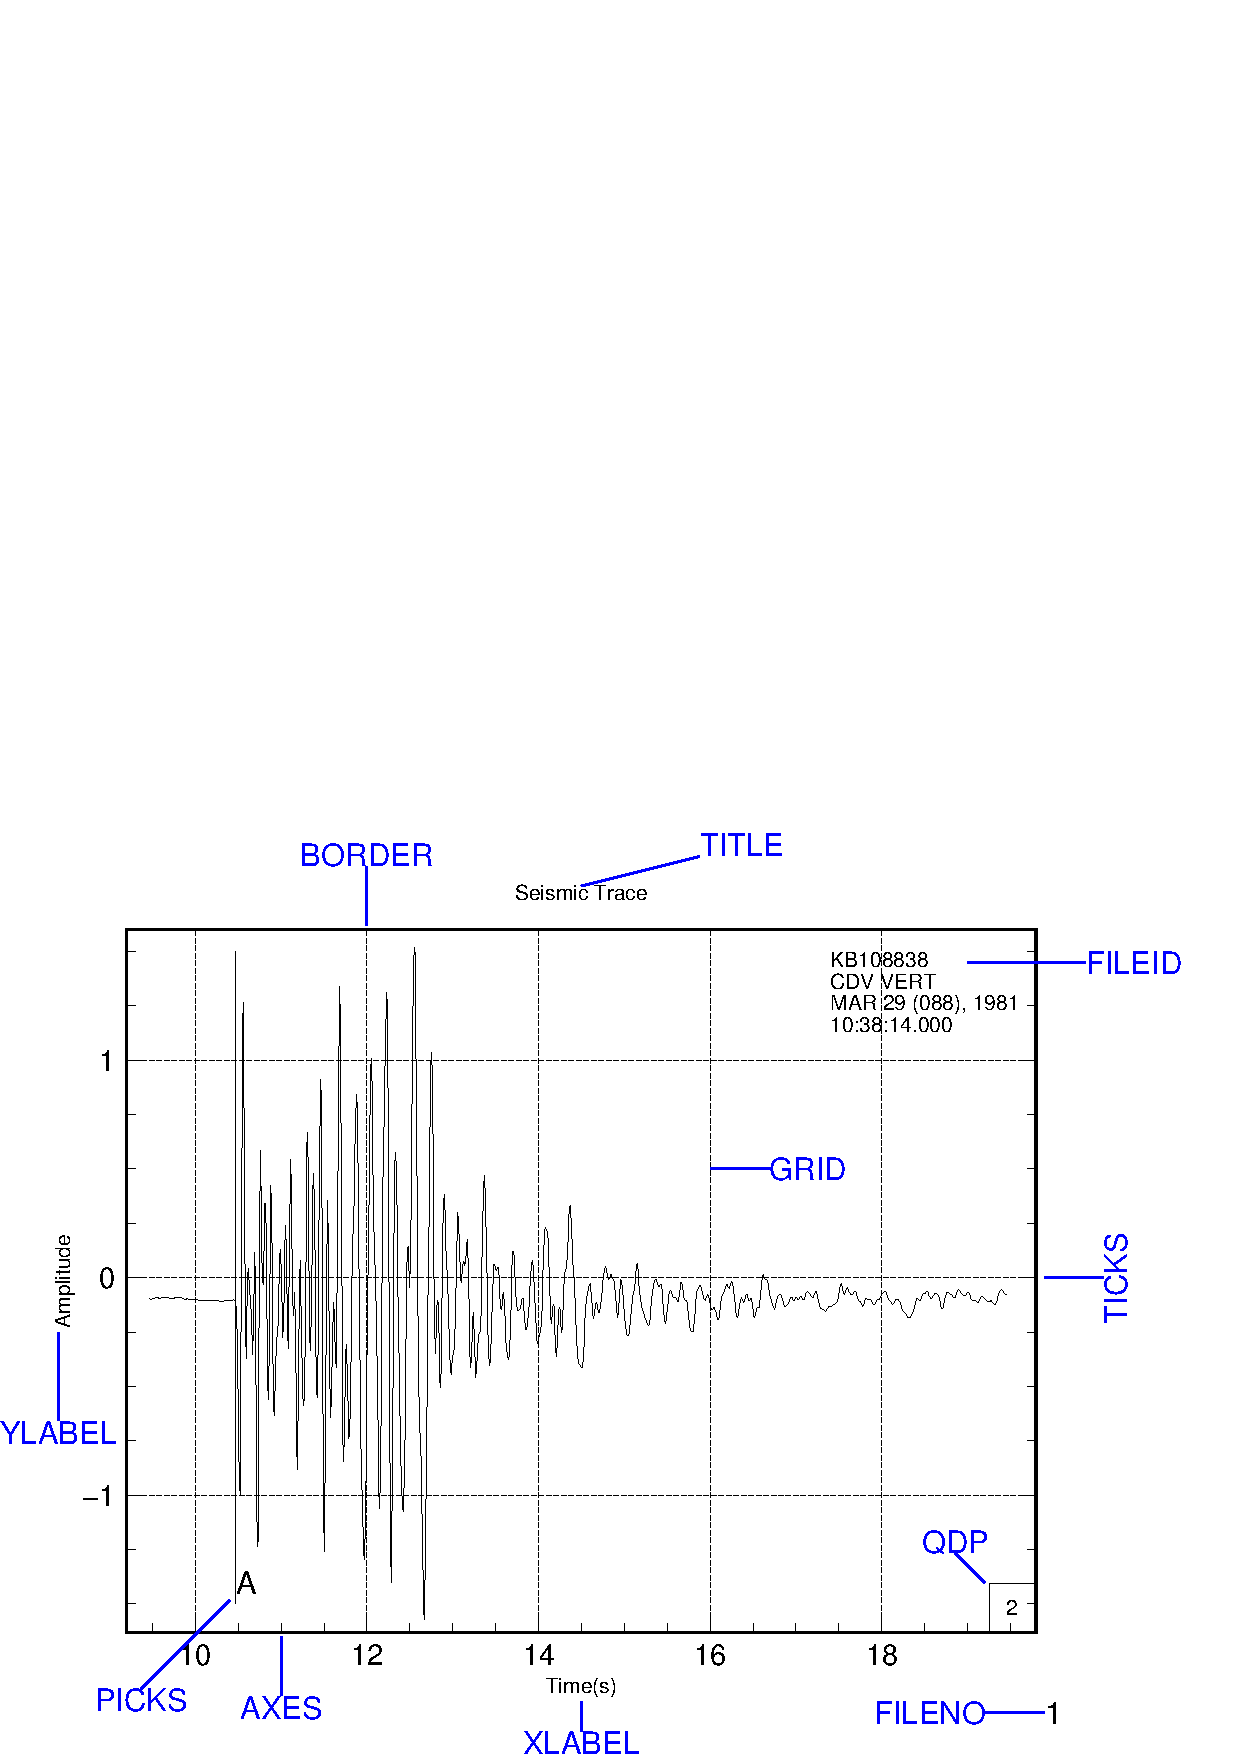
\includegraphics[width=0.9\textwidth]{appearance}
\caption[绘图外观相关命令]{绘图外观及其相关命令。图中蓝色部分为对绘图外观的说明。}
\label{fig:plot-appearance}
\end{figure}

图~\ref{fig:plot-appearance}~可以用如下命令绘制得到:
\begin{SACCode}
SAC> fg seis                // 生成数据
SAC> qdp on                 // 打开QDP选项(默认值即为开)
SAC> grid on                // 显示网格                                          
SAC> title 'Seismic Trace'  // 设置标题                                          
SAC> xlabel "Time(s)"       // 设置x轴标签                                          
SAC> ylabel "Amplitude"     // 设置y轴标签                                       
SAC> filenumber on          // 显示文件号                                       
SAC> axes only left bottom  // left和bottom显示axes
SAC> ticks only right       // right显示ticks    
SAC> border on              // top显示border                                     
SAC> p                      // 绘图
\end{SACCode}

图像中显示的元素包括:
\subsubsection{标签}
标签大致可以分为三种:标题、轴标签和通用标签。
\begin{description}
\item[TITLE] 图像的标题。\nameref{cmd:title}命令可控制标题文本、位置和尺寸
\item[XLABEL、YLABEL] 轴标签。\nameref{cmd:xlabel}和\nameref{cmd:ylabel}命令可
    指定X和Y轴标签文本、位置和尺寸。
\item[PLABEL] 通用标签。\nameref{cmd:plabel}可指定通用标签的文本、位置和尺寸。
\end{description}

标签文本需要用单引号或双引号包围,文本尺寸SIZE可以选择TINY、SMALL、MEDIUM或LARGE,
文本位置LOCATION则可以取TOP、BOTTOM、LEFT或RIGHT。

可以通过\nameref{cmd:plabel}命令定义最多三个通用标签。通用标签与轴标签类似,其
更通用之处在于可以任意指定其位置。每个标签可以用~\verb+POSITION x y a+~来指定
其位置,其中x、y为标签位置相对于窗口尺寸的比例,a表示标签相对于水平方向顺时针旋转
的角度;也可以用~\verb+BELOW+~设置新标签位于上一标签的下方。

\subsubsection{标记}
图像中包含了如下标记:
\begin{description}
\item [FILEID] 文件ID。\nameref{cmd:fileid}用于控制文件ID的内容、位置及其格式。
\item [FILENO] 文件号。\nameref{cmd:filenumber}控制文件号显示与否。
\item [PICKS] 到时标记。\nameref{cmd:picks}用于控制是否显示到时标记以及显示效果。
\item [QDP] QDP因子。\nameref{cmd:qdp}用于控制qdp因子的大小。
\end{description}

QDP,全称为``quick and dirty plot''。在开发SAC的那个年代,计算机的性能一般,
若在绘图时绘制全部数据点,则绘图过程会耗费大量时间。因而SAC采用了``qdp''的方式:
每隔若干个数据点绘制一个数据点\footnote{本质上就是绘图时的一次``减采样'',但是没有做抗混淆处理。}。
图中右下角的``2''即表示每两个点中绘制一个点。
目前计算机的性能已经足够强大,因而一般使用~\verb+qdp off+~命令关于该选项。

\subsubsection{框架}
每张图都有一个框架,每个框架有TOP、BOTTOM、LEFT和RIGHT四条边。

SAC中,每条边都可以用四种不同的形式表示:
\begin{itemize}
\item 不绘制;
\item border:仅一条直线,即图\ref{fig:plot-appearance}中TOP边;
\item ticks:直线+刻度\footnote{刻度专指每条边上的短线。},即图中RIGHT边;
\item axes:直线+刻度+标注\footnote{标注专指每条边上的数字。},即图中LEFT边和BOTTOM边;
\end{itemize}

从上面的定义可以看到,四种形式的边存在包含与被包含的关系,因而在设定边时,有如下规则:
\begin{enumerate}
\item 用\nameref{cmd:axes}控制在哪些边使用``axes'';
\item 只有不使用``axes''的边才可以用\nameref{cmd:ticks}命令控制是否使用``ticks'';
\item 只有不使用``axes''和``ticks''的边才可以使用\nameref{cmd:border}命令控制是否使用``border'';
\item 不使用``axes''、``ticks''和``borders''的边则不绘制。
\end{enumerate}

除了边之外,还可以使用\nameref{cmd:grid}命令控制网格的显示以及网格的线型,或使用
\nameref{cmd:xgrid}、\nameref{cmd:ygrid}分别控制横、纵方向网格的显示和属性。

\subsection{图像控制}
\subsubsection{坐标轴}
SAC使用了优秀的默认算法,根据要绘制的数据范围选择合适的刻度间隔和标注。若对于默认
的结果不满意,可以使用SAC提供的命令分别对X、Y坐标轴进行调整,下面仅列出与X轴相关的
命令。
\begin{description}
\item [xlim] 控制绘图的X轴范围
\item [xdiv] 控制X轴刻度间隔
\item [xfudge] 设定fudge因子,根据数据极值扩展X轴范围
\end{description}

\subsubsection{坐标系}
绘制时间序列一般使用线性坐标系,SAC也提供了一系列命令以指定X、Y轴为线性坐标轴或
对数坐标轴。这些命令包括: \nameref{cmd:linlin}、\nameref{cmd:linlog}、\nameref{cmd:loglin}、
\nameref{cmd:loglog}、\nameref{cmd:xlin}、\nameref{cmd:xlog}、\nameref{cmd:ylin}、
\nameref{cmd:ylog}。

对于对数坐标轴,还有一些命令可以控制其外观,比如\nameref{cmd:xfull}、\nameref{cmd:loglab}、
\nameref{cmd:floor}。

\subsection{线条属性}
\label{subsec:line-attribution}

线条的属性包括线型(\nameref{cmd:line})、线宽(\nameref{cmd:width})、
颜色(\nameref{cmd:color})和符号(\nameref{cmd:symbol})。

下面的命令展示了如何修改线条的属性。
\begin{SACCode}
SAC> fg seis
SAC> line 3         // 线型为3
SAC> width 2        // 线宽为2
SAC> color red      // 红色
SAC> p
\end{SACCode}

\begin{figure}[H]
\centering
\includegraphics[width=0.7\textwidth]{attribution1}
\caption{线条属性}
\end{figure}

在绘制多个波形数据时,可以设置线条的属性按照某个列表递增。下面的命令一次绘制四个
波形文件,使每个数据的线型和颜色都按照默认列表递增。
\begin{SACCode}
SAC> dg sub teleseis ntkl.z nykl.z onkl.z sdkl.z
SAC> line incre
SAC> color black incre
SAC> p
\end{SACCode}

\begin{figure}[H]
\centering
\includegraphics[width=0.7\textwidth]{attribution2}
\caption{线条属性递增}
\end{figure}

\nameref{cmd:line}命令不仅可以设置线条的线型,同时可以对波形数据进行颜色填充:
\begin{SACCode}
SAC> fg seis
SAC> qdp off
SAC> rmean; rtr; taper
SAC> line 0 fill red/blue
SAC> p 
\end{SACCode}

\begin{figure}[H]
\centering
\includegraphics[width=0.7\textwidth]{linefill}
\caption{颜色填充图}
\end{figure}

\input{./graphics/plot-contour.tex}
\section{组合图}
\label{sec:composite-plots}

前面介绍的绘图命令五花八门,但无论是plot、plot1或是plot2,同一个窗口内绘制的
所有波形总是共用同一个X轴。实际绘图时,经常需要在一张图中绘制多个不同X轴的图,
即组合图。

SAC提供了绘制组合图的功能,这其中牵涉到一些新的概念,其中之一是~\verb+frame+~。
一般而言,在执行绘图命令时会首先对整个窗口进行擦除。比如,先执行plot命令,窗口中
会显示出相应的波形,然后执行plot1命令,首先会将窗口中的已有图像全部擦除,再绘制
相应波形。

在frame中,每次执行绘图命令时,不会擦除窗口中的已有图像,从而实现了将多个命令的
绘图效果同时显示在一个窗口中。使用~\nameref{cmd:beginframe}~打开frame时,首先会
擦除整个窗口,进入``组合图模式'';当组合图绘制完成时,需要使用~\nameref{cmd:endframe}~
命令关闭frame。

除了frame之外,在绘制组合图时还需要了解与窗口有关的几个概念,如图
~\ref{fig:window-viewspace-viewport}:
\begin{itemize}
\item window:图形窗口。对于xwindows图形设备,window如图~\ref{fig:plot}~所示,
    其默认长宽比为11.0/8.5=1.294;对于sgf图形设备,可以认为window的大小即为A4纸张的大小。
\item viewspace:window内可以用于绘图的部分;
\item viewport:执行单个绘图命令时,图像的显示区域;
\end{itemize}

\begin{figure}[H]
\centering
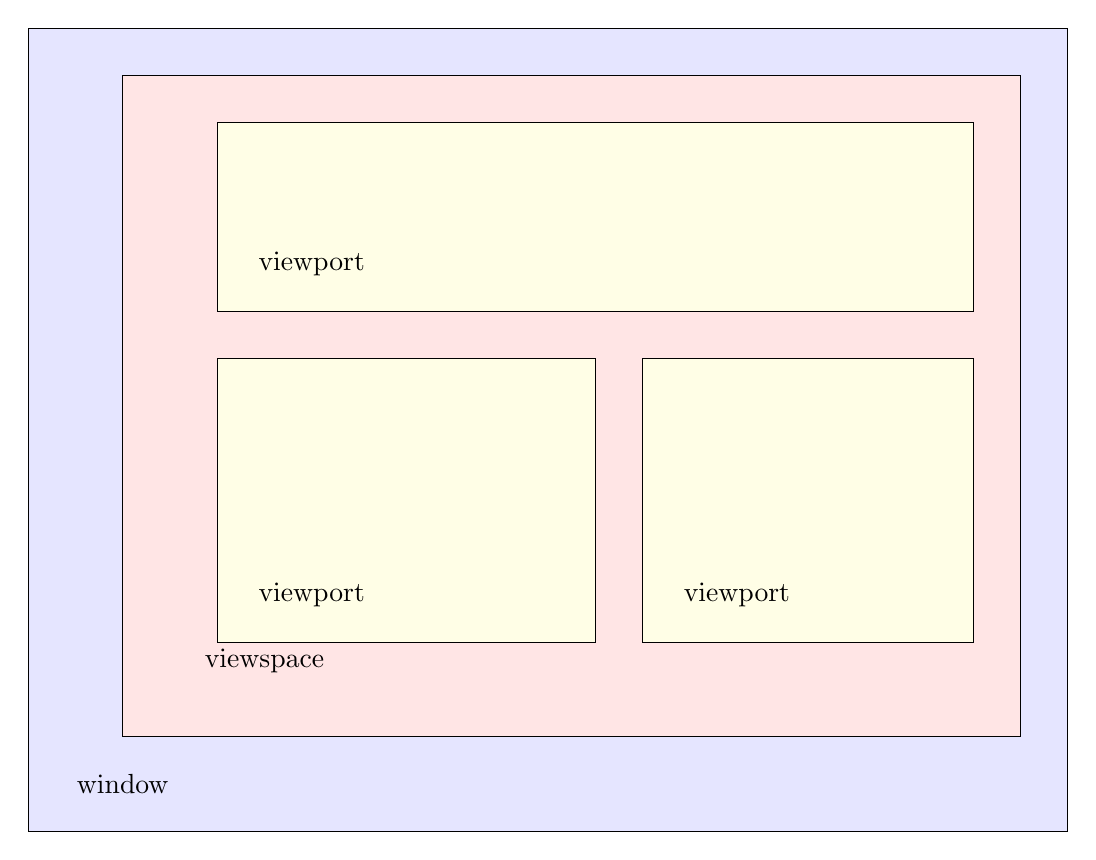
\begin{tikzpicture}[scale=1.2]
    \draw[fill=blue!10] (0,0) rectangle (11.0,8.5);
    \draw[fill=red!10] (1.0,1.0) rectangle (10.5,8);
    \draw[fill=yellow!10] (2,5.5) rectangle (10,7.5);
    \draw[fill=yellow!10] (2,2.0) rectangle (6,5.0);
    \draw[fill=yellow!10] (6.5,2.0) rectangle (10,5.0);
    \draw (1,0.5) node {window};
    \draw (2.5,1.8) node {viewspace};
    \draw (3.0,6) node {viewport};
    \draw (3.0,2.5) node {viewport};
    \draw (7.5,2.5) node {viewport};
\end{tikzpicture}
\caption{window、viewspace和viewport}
\label{fig:window-viewspace-viewport}
\end{figure}

图~\ref{fig:window-viewspace-viewport}~中给出了window、viewspace、viewport的相关
关系。可以使用~\nameref{cmd:window}~命令设定窗口相对于整个屏幕的位置以及X、Y方向
的范围;\nameref{cmd:vspace}~用于设定整个绘图区的比例;\nameref{cmd:xvport}~和
~\nameref{cmd:yvport}~则分别定义了单个绘图命令所能使用的X、Y方向的范围。

一个典型的组合图的绘制如下所示:
\begin{SACCode}
SAC> fg seis                        // 生成数据
SAC> beginframe                     // 打开frame,开始绘制组合图
SAC> xvport 0.1 0.9                 // 设定第一个绘图命令的viewport
SAC> yvport 0.7 0.9                 
SAC> title 'Seismic Trace'          // 设定标题
SAC> fileid off                     // 不显示文件id
SAC> qdp off                        
SAC> p                              
SAC> fft wmean                      // FFT
SAC> xvport .1 .45                  // 设定第二个绘图命令的viewport
SAC> yvport .15 .55
SAC> title 'Amplitude Response (linlog)'
SAC> ylim 1e-5 1                    // Y轴范围
SAC> psp am linlog                  // 绘制振幅谱(linlog)
SAC> xvport .55 .9                  // 设定第三个绘图命令的viewport
SAC> title 'Amplitude Response (loglog)'
SAC> xlim 1 60
SAC> psp am loglog                  // 绘制振幅谱(loglog)
SAC> endframe                       // 关闭frame
\end{SACCode}

\begin{figure}[H]
\centering
\includegraphics[width=0.9\textwidth]{composite-plot}
\caption{绘制组合图}
\label{fig:composite-plot}
\end{figure}

\input{./graphics/save-image}
\section{图像格式转换}
\label{sec:format-conversion}

SAC中的图像可以保存为SGF、PS和PDF格式,有些时候会需要将其转换为其他图像格式,比如JPG或PNG。

\verb+convert+~是Linux下的一个功能强大的图像格式转换工具。如果你的系统里没有这个命令,你可以通过安装~\verb+ImageMagick+~来获取该命令。

convert命令的选项众多,这里只说其中几个常用的选项:

\begin{itemize}
\item \verb+-trim+:切边,即将图像周围多余的白边切除;
\item \verb+-density+ \textit{width}\verb+x+\textit{height}:设置图像精度,一般情况下,设置width为300即可,height可以不指定。
\item \verb+-rotate+ \textit{degree}:图像旋转的角度;
\end{itemize}

下面给出一个简单的例子:

\begin{minted}{console}
    convert -trim -density 300x300 -rotate 90 image.ps image.png
\end{minted}



\chapter{SAC编程}
\label{chap:sac-programming}
\input{./macros/intro-to-sac-programming}
\section{引用头段变量值}
前面已经介绍了SAC中的很多头段变量,也知道如何使用~\nameref{cmd:listhdr}~查看头段
变量的值,lh命令的输出对于人来说很直观,但是对于机器来说却很不友好。有些时候需要
直接使用头段变量的值,这就需要一些特殊的技巧。

最常见的情况是第~\pageref{code:origin-time}~页给出的例子。在使用``ch o gmt''指定发震
时刻后,需要获取头段变量o的值,对该值取负值,并用于``ch allt''中。

在这个例子中,我们需要知道头段变量o的值,并将其值用于其它命令中,准确的说这叫变量
值的引用。在SAC命令中引用SAC头段变量的值有两种方式,分别是~``\verb+&fname,header&+''~
和~``\verb+&fno,header&+''~
\footnote{实际上,SAC官方文档给出的引用方式中没有末尾的~\verb+&+~符号,仅当
一些特殊的情况下才使用,这样容易使得整个语法混乱不堪,所以这里采用了另外一种引用
方式。所有示例均已通过测试。}
。

fname和fno都唯一指向了内存中的某个波形数据,其中fname表示文件名,fno表示文件号
(即内存中的第几个文件,索引值从1开始),header则为头段变量名。

下例展示了如何通过两种方式引用头段变量的值:
\begin{SACCode}
SAC> fg seis
SAC> w seis.SAC
SAC> r ./seis.SAC               // 注意"./"
SAC> lh kevnm o stla            // 查看三个头段变量的值

  FILE: ./seis.SAC - 1          // 这里给出了文件名和文件号
 ----------------

     kevnm = K8108838
         o = -4.143000e+01
      stla = 4.800000e+01
SAC> echo on processed          // 打开回显,显示处理信息
SAC> ch kuser0 &1,kevnm&        // 通过文件号引用头段变量kevnm
 ==>  ch kuser0 K8108838        // 实际执行的效果
SAC> ch user0 &./seis.SAC,o&    // 利用文件名,引用头段变量o
 ==>  ch user0 -41.43
SAC> ch user1 &seis.SAC,stla&   // 文件名少了"./"
 ERROR 1363: Illegal data file list name: seis.SAC
SAC> lh kuser0 user0 user1

  FILE: ./seis.SAC - 1
   ----------------

     kuser0 = K8108838
     user0 = -4.143000e+01
\end{SACCode}

在通过文件名指定波形数据时要注意:SAC记录的是文件的全路径。一般情况下,使用
文件号会更方便些。

\section{黑板变量}
既然是SAC编程,就必然少不了变量,SAC中的变量称之为黑板变量。

黑板变量是SAC中用于临时储存和取回信息而设计的。
黑板变量不需要声明即可直接使用,可以用~\nameref{cmd:setbb}~和~\nameref{cmd:evaluate}~
命令给黑板变量赋值,用~\nameref{cmd:getbb}~获取黑板变量的值。也可以用~\nameref{cmd:writebbf}~
将黑板变量保存在磁盘文件中,然后使用~\nameref{cmd:readbbf}~命令重新将这些变量读入SAC中。


引用黑板变量的值的方式为:~``\verb+%bbvname%+''~,其中bbvname为黑板变量的变量名。

\begin{SACCode}
SAC> echo on processed
SAC> fg seis
SAC> p
SAC> setbb low 2.45         // 黑板变量low=2.45
SAC> setbb high 4.94        // 黑板变量high=4.94
SAC> bp c %low% %high%      // 引用黑板变量low和high的值作为滤波的频带
 ==>  bp c 2.45 4.94        // echo on processed 显示代入值后的命令
SAC> p
SAC> getbb low high         // 查看黑板变量的值
 low = 2.45
 high = 4.94
\end{SACCode}

下例展示了如何将黑板变量写入磁盘文件,等需要时再从磁盘文件中获取:
\begin{SACCode}
$ sac
SAC> setbb var1 10          // 整型
SAC> setbb var2 "text"      // 字符串
SAC> setbb var3 0.2         // 浮点型
SAC> wbbf bbf.file          // 写入到文件
SAC> q
$ ls
bbf.file
$ sac
SAC> readbbf ./bbf.file
SAC> getbb
 NUMERROR = 0
 SACERROR = 'FALSE'
 SACNFILES = 0
 VAR1 = 10
 VAR2 = 'text'
 VAR3 = 0.2
SAC> getbb var2 var3
 var2 = 'text'
 var3 = 0.2
SAC> q
\end{SACCode}

\section{内联函数}

内联函数是SAC实现的一些函数,其可以在SAC命令中使用。在执行命令时,内联函数会首先被
调用,内联函数的结果将替代命令中的内联函数的位置。

SAC提供了如下几类内联函数:
\begin{itemize}
\item 算术运算符;
\item 常规算术运算函数;
\item 字符串操作函数;
\item 其他函数;
\end{itemize}

所有的内联函数的共同形式是:~``\verb+(func)+''~,其中func为内联函数名。某种程度
上,内联函数与前面说到头段变量(``\verb+& &+'')和黑板变量(``\verb+% %+'')类似,
可以认为是通过~``\verb+( )+''~引用了内联函数的结果或值。

内联函数支持嵌套,目前最多可以嵌套10层。

\subsection{算术运算符}
算术运算符即常规的加减乘除运算符,但又有不同,其一般形式如下:
\begin{SACCode}
    ( number operator number )
\end{SACCode}
所有的操作数都被认为是实型的,所有的算术运算都按照双精度浮点型进行运算;

SAC支持的操作符是包括:``\verb+ +  -  *  /  ** +''

看几个简单的例子:
\begin{SACCode}
SAC> echo on
SAC> setbb var1 4+7             // 忘记加括号了!"4+7"被当成了字符串
 setbb var1 4+7
SAC> setbb var2 (4+7)
 setbb var2 (4+7)
 ==>  setbb var2 11             // 4+7=11
SAC> setbb var3 (4+7/3)         // 优先级正确
 setbb var3 (4+7/3)
 ==>  setbb var3 6.33333
SAC> setbb var4 ((4+7)/3)       // 括号改变优先级
 setbb var4 ((4+7)/3)           // 可以看作是内联函数的嵌套
 ==>  setbb var4 3.66667
SAC> setbb var1 ( ( 4 + 7 ) / 3 )   // 支持空格
 setbb var1 ( ( 4 + 7 ) / 3 )
 ==>  setbb var1 3.66667
\end{SACCode}

\subsection{常规算术运算函数}
SAC提供了20个常规算术运算函数,其基本形式为~``\verb+(func arg1 arg2 ...)+''~。
具体函数如表~\ref{table:regular-arithmetic-functions}所示。

\begin{table}[!ht]
\centering
\ttfamily
\small
\caption{常规算数运算函数}
\label{table:regular-arithmetic-functions}
\begin{tabular}{lll}
	\toprule
	命令	&	语法	&	功能	\\
	\midrule
	add		&	( add v1 v2 ... vn )	    &	v1+v2+...+vn	\\
	subtract&	( subtract v1 v2 ... vn )   &	v1-v2-...-vn	\\
	multiply&	( multiply v1 v2 ... vn )   &	v1*v2*...*vn	\\
	divide	&	( divide v1 v2 ... vn )	    &	v1/v2/.../vn	\\
	absolute&	( absolute v )			    &	取绝对值	\\
	power	&	( power v )				    &	取10的v次方     \\
	alog10	&	( alog10 v)				    &	以10为底取v的对数	\\
	alog	&	( alog v)				    &	取v的自然对数	\\
	exp	    &	( exp v)				    &	取e的v次方	\\
	sqrt	&	( sqrt v) 				    &	求v的平方根	\\
	pi		&	( pi )					    &	返回pi值	\\
    sine    &	( sine v )				    &	正弦(v为弧度,下同)\\
	cosine	&	( cosine v )				&	余弦	\\
    tangent	&	( tangent v )			    &	正切	\\
	arcsine	&	( arcsine v )			    &	反正弦	\\
	arccosine&	( arccosine v ) 			&	反余弦	\\
	arctangent&	( arctangent v )			&	反正切	\\
    integer &	( integer v )			    &	取整	\\
	maximum	&	( maximum v1 v2 ... vn )	&	求最大值	\\
	minimum	&	( minimum v1 v2 ... vn )	&	求最小值	\\
	\bottomrule
\end{tabular}
\end{table}

演示如下:
\begin{SACCode}
SAC> echo on processed
SAC> setbb var1 (add 1 3 4)         // 1+3+4
 ==>  setbb var1 8
SAC> setbb var2 (subtract 1 3 4)    // 1-3-4
 ==>  setbb var2 -6
SAC> setbb var3 (multiply 1 3 4)    // 1*3*4
 ==>  setbb var3 12
SAC> setbb var4 (divide 1 3 4)      // 1/3/4
 ==>  setbb var4 0.0833333
SAC> setbb var5 ( absolute -5.1 )   // abs(-5.1)
 ==>  setbb var5 5.1
SAC> setbb var6 ( power 5 )         // 10^5
 ==>  setbb var6 100000
SAC> setbb var7 ( alog10 10000 )    // log10(10000)
 ==>  setbb var7 4
SAC> setbb var8 ( alog 10000 )      // ln(10000)
 ==>  setbb var8 9.21034
SAC> setbb var9 ( exp 5 )           // e^5
 ==>  setbb var9 148.413
SAC> setbb var10 ( sqrt 9 )         // sqrt(9)
 ==>  setbb var10 3
SAC> setbb var11 ( pi )             // PI
 ==>  setbb var11 3.14159
 SAC> setbb var12 ( sine (pi/6) )   // sin(30)
 ==>  setbb var12 0.5
SAC> setbb var13 ((arcsine 0.5)*180/(pi))
 ==>  setbb var13 30
SAC> setbb var14 (integer 3.11)
 ==>  setbb var14 3
SAC> setbb var15 (max 3.11 -1.5 5)  // maximum简写为max
 ==>  setbb var15 5
SAC> setbb var16 (min 3.11 -1.5 5)  // minimum简写为min
 ==>  setbb var16 -1.5
\end{SACCode}

为了对一组数据做归一化,首先要找到所有数据中的绝对最大值,如下:
\begin{SACCode}
SAC> r file1 file2 file3 file4
SAC> echo on processed
SAC> setbb vmax (max &1,depmax& &2,depmax& &3,depmax& &4,depmax&)
 ==> setbb vmax 1.87324
SAC> setbb vmin (min &1,depmin& &2,depmin& &3,depmin& &4,depmin&)
 ==> setbb vmin -2.123371
SAC> div ( max (abs %vmax%) (abs %vmin%) )      // 嵌套
 ==>  div 2.123371
\end{SACCode}
此例可以通过多重嵌套的方式在单个命令中完成,但上面的写法可读性更强。

\subsection{字符串操作函数}
SAC提供了若干个函数用于字符串的处理,如表~\ref{table:string-operation-functions}~所示:

\begin{table}[!ht]
\centering
\ttfamily
\small
\caption{字符串操作函数}
\label{table:string-operation-functions}
\begin{tabular}{lll}
	\toprule
	命令	&	语法(简写形式)	&	功能	\\
	\midrule
	change		&	( cha s1 s2 s3 ) 	&	在s3中用s1代替s2	\\
	substring 	&	( substring n1 n2 s ) 	&	取s中第n1到第n2个字符\\
	delete		&	( del s1 s2 )		&	从s2中删去s1	\\
	concatenate &	( conc s1 s2 ... sn )	&	将多个字符串拼接起来 \\
	before		&	( bef s1 s2)			&	得到s2中位于s1前的部分字符串\\
	after		&	( aft s1 s2 )			&	得到s2中位于s1后的部分字符串\\
	reply		&	( rep s1 )			&	发送信息s1到终端并得到回应	\\
	\bottomrule
\end{tabular}
\end{table}

下面的例子展示了部分函数的用法:
\begin{SACCode}
SAC> echo on processed
SAC> setbb var1 (cha short long "this is short")
 ==>  setbb var1 this is long
SAC> set var2 (del def abcdefghi)
 ==>  set var2 abcghi
SAC> set var4 (before de abcdefg)
 ==>  set var4 abc
SAC> set var4 (after de abcdefg)
 ==>  set var4 fg
SAC> fg seis
SAC> setbb month (substring 1 3 &1,kzdate&)
 ==>  setbb month MAR
SAC> setbb val "1234567890"
SAC> message (substring 1 5 %val%)
 ==>  message 12345
 12345
\end{SACCode}

下面的例子展示concatenate函数的用法以及如何灵活定义标题:
\begin{SACCode}
SAC> fg seis
SAC> echo on processed
SAC> setbb var (conc Seismogram of &1,kevnm& &1,kstnm&)
 ==>  setbb var SeismogramofK8108838CDV                 // 没有空格
SAC> setbb var (conc "Seismogram of " &1,kevnm& " " &1,kstnm&)
 ==>  setbb var Seismogram of K8108838 CDV              // 含空格
SAC> getbb var
 var = 'Seismogram of K8108838 CDV'
SAC> title (conc "Seismogram of " &1,kevnm& " " &1,kstnm&)
 ==>  title Seismogram of K8108838 CDV                  // 错误标题!
SAC> title '(conc "Seismogram of " &1,kevnm& " " &1,kstnm&)'
 ==>  title "(conc "Seismogram of " K8108838 " " CDV)"  // 错误标题!
SAC> title "Seismogram of &1,kevnm& &1,kstnm&"
 ==>  title "Seismogram of K8108838 CDV"                // 正确标题!
\end{SACCode}

下面的例子使用reply函数实现了交互:
\begin{SACCode}
SAC> fg seis
SAC> echo on processed
SAC> rmean; rtr; taper
SAC> setbb low (reply "Enter low freqency limit for bandpass: ")
Enter low freqency limit for bandpass: 2.1          // 用户输入2.1
 ==>  setbb low 2.1
SAC> setbb high (reply "Enter low freqency limit for bandpass: ")
Enter low freqency limit for bandpass: 6.5          // 用户输入6.5
 ==>  setbb high 6.5
SAC> bp c %low% %high%
 ==>  bp c 2.1 6.5
\end{SACCode}

下面的例子中reply函数包含了一个默认值值:
\begin{SACCode}
SAC> setbb bbday (reply "Enter the day of the week: [Monday]")
Enter the day of the week: [Monday]Tuesday      // 用户输入Tuesday
SAC> getbb bbday
 bbday = 'Tuesday'
SAC> setbb bbday (reply "Enter the day of the week: [Monday]")
Enter the day of the week: [Monday]             // 用户无输入
SAC> getbb bbday
 bbday = 'Monday'
\end{SACCode}
当reply函数执行时,引号中的字符串将出现在屏幕上,提示用户输入。如果用户输入,SAC会将
输入的字符串作为返回值,如果用户只是敲击回车键,SAC则会使用该默认值``MONDAY''。

\subsection{其他函数}
这类函数目前只有一个:gettime,其语法为~``\verb+(gettime max|min [value])+~。

gettime函数用于返回数据中首先出现大于或小于value的时间相对于文件参考时刻的相对时间;
若没有指定value,max会返回文件中第一个最大值的相对时间,min会返回文件中第一个最小值
的相对时间。

对于所有的文件有一个最大振幅,要找到这些文件中第一个文件中第一次大于该值所对应的时
间偏移量:
\begin{SACCode}
SAC> fg seis
SAC> echo on processed
SAC> setbb maxtime (gettime max)
 ==>  setbb maxtime 12.55
SAC> setbb mintime (gettime min)
 ==>  setbb mintime 12.67
\end{SACCode}

为了找到第一个大于或等于1.0的数据点的时间偏移,可以使用如下命令:
\begin{SACCode}
SAC> fg seis
SAC> echo on processed
SAC> setbb valuetime ( gettime max 1.0 )
 ==> setbb valuatime 10.55
\end{SACCode}

\section{SAC宏}
\label{sec:macros}

\subsection{简单的例子}
假如你有一些重复的工作需要完成,那么SAC宏显然可以帮你节省不少时间。例如,要经常
读取三个文件ABC、DEF和XYZ,每个文件分别乘以不同的值,做Fourier变换,然后将频谱的
振幅部分绘制到SGF文件中,这样的一系列命令可以写入到SAC宏文件中:
\begin{SACCode}
** This certainly is a simple little macro.
r ABC DEF XYZ
mul 4 8 9
fft
bg sgf
psp am
\end{SACCode}

假设上面的代码保存到文件mystuff中,且该文件位于当前目录中,可以通过下面的命令执行该宏文件:
\begin{SACCode}
SAC> macro mystuff
\end{SACCode}
终端中并不会显示正在执行的宏文件中的命令,可以使用echo命令来设置在终端显示哪些东西。
另外,若某行的第一列为星号则该行为注释行,SAC不会去执行注释行。

\subsection{宏搜索路径}
当你执行一个宏文件而又没有给出宏文件的绝对路径时,SAC会按照下面的路径顺序搜索宏文件:
\begin{enumerate}
\item 在当前目录搜索;
\item 在~\nameref{cmd:setmacro}~命令设置的搜索目录中搜索;
\item 在SAC的全局宏目录(\texttt{sac/aux/macros})中搜索;
\end{enumerate}

所有人都可以使用全局宏目录中的宏文件,可以使用installmacro命令将自己的宏文件安装到这个目录中。
你也可以通过绝对/相对路径指定搜索路径。

\subsection{宏参数}
如果想要每次读取不同的文件或者乘以不同的值那么必须每次都修改该文件,
让宏文件在执行之前允许用户输入参数可以大大增加宏文件的灵活性。

SAC宏参数的格式为:~``\verb+$n$+'',其中n从1开始。

下面将对先前的宏文件进行修改以使其可以接收文件名作为参数:
\begin{SACCode}
r $1$ $2$ $3$
mul 4 8 9
fft
bg sgf
psp am
\end{SACCode}
~``\verb+$1$+''~、~``\verb+$2$+''~和~``\verb+$3$+''~分别表示宏文件
接收到的第一、二、三个参数,用下面的命令执行这个宏文件:
\begin{SACCode}
SAC> macro mystuff ABC DEF XYZ
\end{SACCode}

可以用下面的命令再次执行这个宏文件,但读取不同的文件:
\begin{SACCode}
SAC> macro mystuff AAA BBB CCC
\end{SACCode}

\subsection{关键字驱动参数}
关键字驱动参数允许用户按照任意顺序输入参数,这也使得宏文件的内容变得简单易懂。

当参数的数目以及宏文件的大小不断增大的时候这就变得更加重要了。
下面将再一次修改这个例子以使其可以接受文件列表以及乘数的列表:
\begin{SACCode}
$keys$ files values
r $files$
mul $values$
fft
bg sgf
psp am
\end{SACCode}
\verb+$keys$+~表明``files''和``values''是关键字。可以按照下面的输入来执行这个宏文件:
\begin{SACCode}
SAC> macro mystuff files ABC DEF XYZ values 4 8 9
\end{SACCode}
因为参数的顺序不再重要,所以你可以像下面这样输入:
\begin{SACCode}
SAC> macro mystuff values 4 8 9 files ABC DEF XYZ
\end{SACCode}
这个宏文件并不限于读取三个文件,它对于文件的数目没有限制,只要文件数与值数目相匹配就好。

\subsection{宏参数缺省值}
有些时候会遇到这样的情况,宏文件的有些参数在多次执行的过程中经常但并不总是拥有相同的值。
为这些参数提供缺省值可以减少输入那些相同值的次数同时又保有宏参数本身的灵活性。如下例所示:
\begin{SACCode}
$keys$ files values
$default$ values 4 8 9
r $files$
mul $values$
fft
bg sgf
psp am
\end{SACCode}
\verb+$default$+~指定了宏参数~\verb+values+~的缺省值,若在执行宏文件时不输入
values的参数值那么这些参数将使用缺省值:
\begin{SACCode}
SAC> macro mystuff files ABC DEF XYZ
\end{SACCode}
如果想要使用不同的值,可以像下面这样输入:
\begin{SACCode}
SAC> macro mystuff values 10 12 3 files ABC DEF XYZ
\end{SACCode}

\subsection{参数请求}
若执行宏文件时没有输入参数而这些参数又没有缺省值,SAC会在终端中提示你输入相应的参数值。
在上面的例子中,如果你忘记输入参数则会出现下面的情况:
\begin{SACCode}
SAC> macro mystuff
files? ABC DEF XYZ          // 用户输入ABC DEF XYZ
\end{SACCode}
注意到SAC 并不会提示输入参数values的值,因为它们已经有了缺省值。SAC并非在一开始就提示输入
参数,其等到需要计算参数值却发现没有缺省值或者输入值时才会提示需要输入该参数。

\subsection{联接}
头段变量、黑板变量、宏参数以及字符串可以直接联接在一起。

\begin{SACCode}
$keys$ station
fg seis
echo on
setbb sta $station$.z
setbb tmp ABC
setbb tmp1 XYZ%tmp%
setbb tmp2 (&1,o&)
setbb fname $station$%tmp%%tmp1%%tmp2%.SAC
\end{SACCode}

执行效果如下:
\begin{SACCode}
SAC> m stuff station STA
 setbb sta $station$.z
 ==>  setbb sta STA.z
 setbb tmp ABC
 setbb tmp1 XYZ%tmp%
 ==>  setbb tmp1 XYZABC
 setbb tmp2 @(&1,o&@)
 ==>  setbb tmp2 (-41.43)
 setbb fname $station$%tmp%%tmp1%%tmp2%.SAC
 ==>  setbb fname STAABCXYZABC(-41.43).SAC
\end{SACCode}

\subsection{条件判断}
条件判断在任何一个编程语言中都是必不可少的,SAC宏的条件判断语句与Fortran77类似,
但不完全相同,要注意区分。

SAC宏的条件判断格式如下:
\begin{SACCode}
  IF expr
  	commands
  ELSEIF expr
  	commands
  ELSE
  	commands
  ENDIF
\end{SACCode}

逻辑表达式expr具有如下形式:
\begin{SACCode}
    token 关系运算符 token
\end{SACCode}
其中token可以是一个常数、宏参数、黑板变量或头段变量,关系运算符则是GT、GE、LE、LT、EQ、NE
中的一个。上面的逻辑表达式在计算之前token会被转换为浮点型数。

条件判断语句目前最多支持10次嵌套,且elseif、else是可选的,elseif的次数没有限制。

下面给出一个例子:
\begin{SACCode}
r $1$
markptp
if &1,user0& ge 2.45
    fft
    psp am
else
    message "Peak to peak for $1 below threshold."
endif
\end{SACCode}
在这个例子中,一个文件被读入内存,markptp测出其最大峰峰值,并保存到头段变量user0中,
若该值大于某一确定值,则对其做Fourier变换并绘制振幅图,否则输出信息到终端。

\subsection{循环控制}
循环特性允许在一个宏文件中重复执行一系列命令。通过固定循环次数、遍历元素列表或者
设定条件来执行一系列命令,也可以随时中断一次循环。
循环的最大嵌套次数为10次。其语法可以有多种形式:
\begin{SACCode}
DO variable = start, stop [,increment]
    commands
ENDDO
\end{SACCode}

\begin{SACCode}
DO variable FROM start TO stop [BY increment]
    commands
ENDDO
\end{SACCode}

\begin{SACCode}
DO variable LIST entrylist
    commands
ENDDO
\end{SACCode}

\begin{SACCode}
DO variable WILD [DIR name] entrylist
    commands
ENDDO
\end{SACCode}

\begin{SACCode}
WHILE expr
    commands
ENDDO
\end{SACCode}
其中大写字符串均为关键字,不可更改:
\begin{itemize}
\item variable是循环变量名,在变量名前后加上~``\verb+$+''~即可在do循环中引用该变量;
\item start、stop、increment 循环变量的初值、终值、增值,start、stop必须为整型数,
    increment缺省值为1
\item entrylist是do循环执行时变量可以取的所有值的集合,值之间以空格分开,其可以为整型、
  浮点型或字符型。DO WILD中entrylist由字符串和通配符构成,循环执行前,这个列表将根据
  通配符扩展为一系列文件名。
\end{itemize}

下面给出一些DO循环的例子:

该宏文件对数据使用了DIF以进行预白化处理,进行Fourier变换,然后使用DIVOMEGA命令去除
预白化的影响,有时需要在做变换之前多次预白化,那么就可以这样写:
\begin{SACCode}
$keys$ file nprew
$default$ nprew 1
r $file
do j = 1 , $nprew$
    dif
enddo
fft amph
do j = 1 , $nprew$
    divomega
enddo
\end{SACCode}

下面这个例子,用相同的数据绘制5个不同的两秒时间窗的质点运动矢量图:
\begin{SACCode}
r abc.r abc.t
setbb time1 0
do time2 from 2 to 10 by 2
    xlim %time1% $time2$
    title 'Particle motion from %time1% to $time2$'
    plotpm
    setbb time1 $time2$
enddo
\end{SACCode}

在下面的例子中,一个宏文件调用另一个名为preview的宏文件,通过do循环以达到多次调用preview的目的:
\begin{SACCode}
do station list abc def xyz
    do component list z n e
        macro preview $station$.$component$
    enddo
enddo
\end{SACCode}

在下面的例子中我们修改上一个宏文件使得其可以处理目录mydir中所有以``.Z''结束的文件:
\begin{SACCode}
do file wild dir mydir *.Z
    macro preview $file$
enddo
\end{SACCode}

最后一个例子有三个参数,第一个是文件名,第二个是一个常数,第三个是一个阀值。宏文件读取了
一个数据文件,然后每个数据点乘以一个常数直到其超过某一阀值:
\begin{SACCode}
r $1$
while &1,depmax& gt $3$
    mul $2$
enddo
\end{SACCode}

另一个与break有关的宏文件:
\begin{SACCode}
r $1$
while 1 gt 0
    div $2
    if &1,depmax& gt $3$
        break
    endif
enddo
\end{SACCode}
这个while循环是一个无限循环,它只能通过break来中断。

\subsection{嵌套与递归}
SAC宏提供嵌套功能,不支持递归,但是SAC并不会去检查宏的调用是否保证不是递归,因而需要
用户去保证宏文件不要直接或间接调用自己。

\subsection{中断宏}
有些时候需要临时中断宏文件的执行,用户自己从终端输入一些命令,然后继续执行宏文件。
这个可以利用SAC的pause和resume特性做到。当SAC在宏文件中遇到~``\verb+$TERMINAL$+''~时它会临时停止
执行宏文件,更改提示符为宏名,然后提示从终端输入命令,然后当SAC在终端中看到~``\verb+$RESUME$+''~
时则会停止从终端读取命令继续从宏文件读取。如果你不想再继续执行宏文件中的命令,可以
在终端输入~``\verb+$KILL$+''~,SAC将关闭宏文件,回到上一层。
在一个宏文件中可以有多个~``\verb+$TERMINAL$+''~中断。

\subsection{调用外部程序}
你可以在SAC宏内部执行其他程序,可以向程序传递参数。如果程序是交互式的
你也可以将输入行发送给它,语法如下:
\begin{SACCode}
$RUN$ program message
inputlines
ENDRUN
\end{SACCode}
宏参数、黑板变量、头段变量、内联函数均可使用,在程序执行之前它们会被计算,当程序执行
结束,SAC宏会在ENDRUN之后继续执行。

\subsection{转义字符}
字符~``\verb+$+''~和~``\verb+%+''在SAC中具有特殊的含义,有时在字符串中需要使用这些
特殊字符,但SAC会将其解释成一个变量,此时就需要使用转义字符,SAC中的转义符为~``\verb+@+''~,
可以被转义的特殊符号包括:
\begin{itemize}
    \item \verb+$+  宏参数标识符
    \item \verb+%+  黑板变量标识符
    \item \verb+&+  头段变量标识符
    \item \verb+@+  转义字符本身
    \item \verb+()+  内联函数起始符
\end{itemize}


\chapter{在脚本中调用SAC}
\label{chap:sac-script}
\section{Bash中调用SAC}
\label{sec:sac-bash}

\subsection{简介}
SAC宏的功能相对比较单一,难以满足日常数据处理的需求,可以在Bash脚本中直接调用SAC,
这样可以利用Bash脚本的更多特性。

下面的例子展示了如何在Bash脚本中调用SAC:
\inputminted{bash}{./call-in-script/simple-script.sh}

SAC在启动是默认会显示版本信息,当用脚本多次调用SAC时,版本信息也会显示多次,可以
通过设置环境变量~``\lstinline{export SAC_DISPLAY_COPYRIGHT=0}''的方式隐藏版本信息。

脚本中从~``\lstinline{sac << EOF}''~开始到~``\lstinline{EOF}''~的全部内容,都会被
Bash传递给SAC,SAC会逐一解释并执行每行命令。

\subsection{头段变量和黑板变量}
想要在Bash脚本中引用头段变量,需要借助于SAC宏的语法。
\inputminted{bash}{./call-in-script/variables.sh}

\subsection{内联函数}
bash可以完成基本的数学运算,但是所有的运算只支持整型数据,浮点型运算或者其它更
高级的数学运算需要借助bc或者awk来完成。Bash中的变量以~``\lstinline{$}''~作为标识符,
Bash会首先做变量替换再将替换后的命令传递给SAC。
\inputminted{bash}{./call-in-script/arithmetic-functions.sh}

本例中的变量~``\lstinline{$var1}''~和~``\lstinline{$var2}''~会首先被SAC解释成
为1和2,因而SAC实际接收到的命令是~``\lstinline{bp c 1 2}''。

借助于awk、sed等工具,也可以实现部分字符串处理函数:
\inputminted{bash}{./call-in-script/string-functions.sh}

\subsection{条件判断和循环控制}
Bash具有更灵活的条件判断和循环控制功能,但由于Bash自身的限制,这些特性仅能
在SAC外部使用,因而下例中需要多次调用SAC,在某些情况下会相当耗时。
\inputminted{bash}{./call-in-script/do-loops.sh}

\section{在Perl中调用SAC}
\label{sec:sac-perl}

\subsection{简介}
下面的脚本中给出了一个简单的例子,展示了如何在Perl中调用SAC。相对于Bash来说,Perl脚本似乎
需要更多的键入,但是相对于Perl的优势来说,这些都不算什么。
\inputminted{perl}{./call-in-script/simple-script.pl}

\subsection{头段变量}
Perl无法直接引用SAC文件的头段变量值,依然需要利用SAC宏的的语法。Perl的优势在于可以
一边向SAC传递信息,一边运行自身的命令。
\inputminted{perl}{./call-in-script/variables.pl}
本例中第9行,在SAC运行的同时Perl临时定义了一个变量,并成功将其传递给了SAC,这在
Bash中是不容易做到的。

\subsection{内联函数}
Perl可以完成各种复杂的数学运算:
\inputminted{perl}{./call-in-script/arithmetic-functions.pl}

Perl对字符串的处理更是Perl的杀手锏:
\inputminted{perl}{./call-in-script/string-functions.pl}

\subsection{条件判断和循环控制}
Perl也可以很容易地实现条件判断和循环控制:
\inputminted{perl}{./call-in-script/do-loops.pl}
这个例子中只启动了一次SAC,然后开始Perl的循环控制,读取当前目录下的每一个SAC文件,
做一些数据处理,然后写到新文件中。

该Perl脚本与上一个Bash脚本相比,实现了几乎相同的功能,但Perl脚本中仅启动和退出SAC
一次,与Bash脚本的多次启动相比,其效率要高很多。

\section{在Python中调用SAC}
\label{sec:sac-python}

\subsection{简介}
下面的脚本中给出了一个简单的例子,展示了如何在Python中调用SAC。
\inputminted{python}{./call-in-script/simple-script.py}

\subsection{头段变量}
Python无法直接引用SAC文件的头段变量值,依然需要利用SAC宏的的语法。但Python不需要使用SAC的黑板变量功能。
\inputminted{python}{./call-in-script/variables.py}
本例中第13行,在SAC运行的同时Python临时定义了一个变量,并成功将其传递给了SAC,这在Bash中是不容易做到的。

\subsection{内联函数}
Python可以完成各种复杂的数学运算:
\inputminted{python}{./call-in-script/arithmetic-functions.py}

Python对字符串的处理也很简单:
\inputminted{python}{./call-in-script/string-functions.py}

\subsection{条件判断和循环控制}
Python也可以很容易地实现条件判断和循环控制:
\inputminted{python}{./call-in-script/do-loops.py}
这个例子中只启动了一次SAC,然后开始Python的循环控制,读取当前目录下的每一个SAC文件,
做一些数据处理,然后写到新文件中。

该Python脚本与上一个Bash脚本相比,实现了几乎相同的功能,但Python脚本中仅启动和退出SAC
一次,与Bash脚本的多次启动相比,其效率要高很多。


\chapter{使用SAC函数库}
\label{chap:sac-libs}
\section{SAC库简介}
SAC提供了两个函数库:libsacio.a和libsac.a,用户可以在自己的C或Fortran程序
中直接使用函数库中的子函数。这些库文件位于~\verb+sac/lib+~中。

\subsection{libsacio库}
这个库文件的子函数可用于读写SAC数据文件、头段变量、黑板变量。这些子函数可以在用户
的C或Fortran程序中直接使用。

libsacio.a中可用的子函数包括:
\begin{table}[H]
\centering
\caption{libsacio子函数}
\ttfamily
\begin{tabular}{ll}
\toprule
子函数      &       说明            \\
\midrule    
rsac1       &       读取等间隔文件  \\
rsac2       &       读取不等间隔文件和谱文件    \\
wsac1       &       写入等间隔文件  \\
wsac2       &       写入不等间隔文件    \\
wsac0       &       可以写等间隔文件或不等间隔文件  \\
getfhv      &       获取浮点型头段变量值    \\
setfhv      &       设置浮点型头段变量值    \\
getihv      &       获取枚举型头段变量值    \\
setihv      &       设置枚举型头段变量值    \\
getkhv      &       获取字符串头段变量值    \\
setkhv      &       设置字符串头段变量值    \\
getlhv      &       获取逻辑型头段变量值    \\
setlhv      &       设置逻辑型头段变量值    \\
getnhv      &       获取整型头段变量值      \\
setnhv      &       设置整型头段变量值  \\
readbbf     &       读取一个黑板变量文件    \\
writebbf    &       写一个黑板变量文件      \\
getbbv      &       获取一个黑板变量的值    \\
setbbv      &       给一个黑板变量赋值      \\
\bottomrule
\end{tabular}
\end{table}

对于C源码,用如下命令编译
\begin{minted}{console}
$ gcc -c source.c -I/usr/local/sac/include
$ gcc -o prog source.o -lm -L/usr/local/sac/lib -lsacio
\end{minted}
也可以利用SAC提供的sac-config命令简化此编译命令:
\begin{minted}{console}
$ gcc -c source.c `sac-config -c`
$ gcc -o prog source.o -lm `sac-config -l sacio`
\end{minted}

对于Fortran77源码,用如下命令编译
\begin{minted}{console}
$ gfortran -c source.f
$ gfortran -o prog source.o -L/opt/sac/lib/ -lsacio
\end{minted}
也可以利用SAC提供的sac-config命令简化此编译命令:
\begin{minted}{console}
$ gfortran -c souce.f
$ gfortran -o prog source.o `sac-config -l sacio`
\end{minted}

\subsection{libsac.a库}
这个库是从101.2版本才引入的,其是libsacio.a的超集,包含了几个数据处理常用的子函数。

libsac.a包含如下子函数:
\begin{itemize}
\item xapiir  无限脉冲响应滤波器;
\item firtrn  有限脉冲滤波器,Hilbert变换;
\item crscor  互相关;
\item next2   返回比输入值大的最小的2的幂次;
\item envelope 计算包络函数; 
\end{itemize}

对于C源码,用如下命令编译
\begin{minted}{console}
$ gcc -c source.c -I/usr/local/sac/include
$ gcc -o prog source.o -lm -L/usr/local/sac/lib -lsac
\end{minted}
也可以利用SAC提供的sac-config命令简化此编译命令:
\begin{minted}{console}
$ gcc -c source.c `sac-config -c`
$ gcc -o prog source.o -lm `sac-config -l sac`
\end{minted}

对于Fortran77源码,用如下命令编译
\begin{minted}{console}
$ gfortran -c source.f
$ gfortran -o prog source.o -L/opt/sac/lib/ -lsac
\end{minted}
也可以利用SAC提供的sac-config命令简化此编译命令:
\begin{minted}{console}
$ gfortran -c souce.f
$ gfortran -o prog source.o `sac-config -l sac`
\end{minted}

\section{调用libsacio库}
\subsection{rsac1}
子函数rsac1用于读取等采样间隔的SAC数据。

函数定义如下:
\begin{minted}{c}
void
rsac1(  char    *kname,     // 要读入的文件名
        float   *yarray,    // 数据被保存到yarray数组中
        int     *nlen,      // 数据长度
        float   *beg,       // 数据开始时间,即头段变量b
        float   *del,       // 数据采样周期,即头段变量delta
        int     *max_,      // 数组yarray的最大长度,若nlen>max_则截断
        int     *nerr,      // 错误标记,0代表成功,非零代表失败
        int      kname_s    // 数组kname的长度
)
\end{minted}

相关示例代码为~\verb+rsac1c.c+~\footnote{代码位于~\verb+sac/doc/examples+,下同。}
和~\verb+rsac1f.f+。

\subsection{rsac2}
子函数rsac2用于读取非等间隔采样的。
\begin{minted}{c}
void
rsac2(  char    *kname,     // 要读入的文件名
        float   *yarray,    // 因变量数组
        int     *nlen,      // 数据长度
        float   *xarray,    // 自变量数组
        int     *max_,      // 数组最大长度
        int     *nerr,      // 错误标记
        int      kname_s    // 数组kname的长度
)
\end{minted}
相关示例代码为~\verb+rsac2c.c+~和~\verb+rsac2f.f+。

\subsection{wsac1}
子函数wsac1用于写等间隔SAC文件。
\begin{minted}{c}
void
wsac1(  char  *kname,       // 要写入的文件名
        float *yarray,      // 要写入文件的数组
        int   *nlen,        // 数组长度
        float *beg,         // 数据起始时刻
        float *del,         // 数据采样周期
        int   *nerr,        // 错误标记
        int    kname_s      // 文件名长度
)
\end{minted}

相关示例代码为~\verb+wsac1c.c+~和~\verb+wsac1f.f+。

\subsection{wsac2}
写非等间隔SAC文件。

\begin{minted}{c}
void
wsac2(  char  *kname,       // 文件名
        float *yarray,      // 因变量数组
        int   *nlen,        // 数组长度
        float *xarray,      // 自变量数组
        int   *nerr,        // 错误码
        int    kname_s      // 文件名长度
)
\end{minted}

相关示例代码为~\verb+wsac2c.c+~和~\verb+wsac2f.f+。

\subsection{wsac0}
子函数wsac0相对来说更加通用也更复杂,利用该函数可以创建包含更多头段的SAC文件。

\begin{minted}{c}
void
wsac0(  char  *kname,       // 文件名
        float *xarray,      // 自变量数组
        float *yarray,      // 因变量数组
        int   *nerr,        // 错误码
        int    kname_s      // 文件名长度
)
\end{minted}

要使用子函数wsac0,首先要调用子函数~\verb+newhdr()+~创建一个完全未定义的头段区,并利用其它
头段变量相关子函数设置头段变量的值,并由wsac0写入到文件中。必须要赋值的头段变量
为delta、b、e、npts、iftype。

相关示例代码为~\verb+wsacnc.c+~、~\verb+wsacnf.f+。n=3,4,5。

\subsection{getfhv}
获取浮点型头段变量的值。
\begin{minted}{c}
void
getfhv( char  *kname,       // 头段变量名
        float *fvalue,      // 浮点型头段变量的值
        int   *nerr,        // 错误码
        int    kname_s      // 变量名长度
)
\end{minted}

相关示例代码为~\verb+gethvc.c+~和~\verb+gethvf.f+。

至于如何获取和设置其它类型的头段变量,方法类似,不再多说。

\subsection{readbbf}
读取一个黑板变量文件。
\begin{minted}{c}
void
readbbf( char   *kname,     // 要读取的文件
         int    *nerr,      // 错误码
         int    kname_s     // 文件名长度
)
\end{minted}

writebbf与之类似,不再列出。

\subsection{getbbv}
获取一个黑板变量的值。
\begin{minted}{c}
void
getbbv( char    *kname,     // 黑板变量名
        char    *kvalue,    // 黑板变量的值
        int     *nerr,      // 错误码
        int     kname_s,    // 变量名长度
        int     kvalue_s    // 变量值的长度
)
\end{minted}
setbbv的函数定义与其类似,不再列出。

\section{调用libsac库}
\label{sec:libsac}
\subsection{next2}
SAC在做FFT时要保证数据点数为$2^n$个,对于不足$2^n$个点的数据需要补零至$2^n$次方个点。

next2函数定义为:
\begin{minted}{c}
int next2(int num)  // 输入为num,返回值为大于num的最小2次幂
\end{minted}

\subsection{xapiir}
xapiir用于设计IIR滤波器,并对数据进行滤波。这个子函数底层调用了design和apply两个
子函数。
\begin{minted}{c}
void
xapiir(float    *data,      // 待滤波的数据,滤波后的数据保存在该数组中
       int       nsamps,    // 数据点数
       char     *aproto,    // 滤波器类型
                            //  - 'BU'  :   butterworth
                            //  - 'BE'  :   bessel
                            //  - 'C1'  :   chebyshev type I
                            //  - 'C2'  :   chebyshev type II
       double    trbndw,    // chebyshev滤波器的过渡带宽度
       double    a,         // chebyshev滤波器的衰减因子
       int       iord,      // 滤波器阶数
       char     *type,      // 滤波类型,'LP','HP','BP','BR'
       double    flo,       // 低频截断频率
       double    fhi,       // 高频截断频率
       double    ts,        // 采样周期
       int       passes     // 通道数,1或2
)
\end{minted}

相关示例代码为~\verb+filterc.c+~和~\verb+filterf.f+~。

\subsection{firtrn}
\begin{minted}{c}
void
firtrn( char    *ftype,     // 类型,取'HILBERT'或'DERIVATIVE'
        float   *x,         // 输入数据
        int      n,         // 数据点数,至少含201个点
        float   *buffer,    // 临时数组,长度至少4297
        float   *y          // 输出数组
)
\end{minted}

参考示例:
\begin{minted}{c}
#include <stdio.h>
#include <stdlib.h>
#define NPTS 1000
float *hilbert(float *in, int npts);
int main(){
    float data[NPTS];
    float *hdata;
    int i;
    // 准备输入数据
    for (i=0; i<NPTS; i++)  data[i] = i;
    // 进行Hilbert变换,hdata为Hilbert变换的结果
    hdata = hilbert(data, NPTS);
    for (i = 0; i < NPTS; i++)
        printf("%f\n", hdata[i]);
}

// 这里定义了hilbert函数,是对firtrn函数的一个封装
float *hilbert(float *in, int npts) {
    float *buffer;
    float *out;
    buffer = (float *)malloc(sizeof(float)*50000);
    out = (float *)malloc(sizeof(float)*npts);
    firtrn("HILBERT", in, npts, buffer, out);
    return out;
}
\end{minted}

\subsection{envelope}
该子函数用于计算数据的包络函数,其底层调用了firtrn函数。
\begin{minted}{c}
void
envelope( int    n,     // 数据点数
          float *in,    // 输入数据
          float *out    // 输出数据
)
\end{minted}

相关示例代码为~\verb+envelopec.c+~和~\verb+envelopef.f+。

\subsection{crscor}
该子函数用于计算两个数据的互相关,此互相关在频率域中完成,相对时间域互相关而言
效率更高。

\begin{minted}{c}
void
crscor( float   *data1,     // 数据1
        float   *data2,     // 数据2
        int      nsamps,    // 数据点数
        int      nwin,      // 相关窗数目
        int      wlen,      // 窗内数据点数,最大值为2048
        char    *type,      // 窗类型,可以取'HAM','HAN','C','R','T'
        float   *c,         // 输出数据,长度为2*wlen-1
        int     *nfft,      // 相关序列的数据点数
        char    *err,       // 错误消息
        int      err_s      // 错误消息长度
)
\end{minted}

示例代码为~\verb+convolvec.c+、~\verb+convolvef.f+、~\verb+correlatec.c+~
和~\verb+correlatef.f+。


% external_howto external_interface

\chapter{SAC I/O自定义}
\label{chap:sac-custom-io}
这一章的内容一直没有想好怎么写,姑且先放在这里,等等再说。

SAC自身已经提供了一系列用于读写SAC文件的子函数,但是函数功能过于单一。
比如读函数只能一次性读取整个文件,无法只读取
文件的一部分(即没有截窗的功能);再比如,想要获取多个头段变量的值,必须
多次调用相应的子函数。

在理解了SAC的内部结构之后,可以完全自定义SAC I/O函数库。

Prof. Lupei Zhu实现了一个比较方便的SAC I/O函数库,可以直接使用或者作为参考。
相关地址为:\url{http://www.eas.slu.edu/People/LZhu/downloads/pssac.tar}。

另一方面,我自己正在计划重写SAC I/O函数库以及相应的一些辅助工具。重写SAC I/O
函数库的原因在于Prof. Lupei Zhu的I/O库中存在一些潜在的Bug以及考虑不周之处,并且
现有的诸如saclst等辅助工具功能尚有欠缺。

该项目目前还是玩具性质,仅供参考:\url{https://github.com/seisman/sac_tools}。


\chapter{SAC相关工具}
\input{./sac-tools/byte-swap}
\section{sgftops}
\label{sec:sgftops}
\label{sec:sgftoeps}
\label{sec:sgftox}

SGF格式是SAC自定义的图像文件格式,转换到常见的其他图像格式,需要使用转换工具sgftops。

sgftops可以将SGF格式的文件转换为PS格式。其用法如下:
\begin{minted}{console}
$ sgftops
Usage: sgftops sgf_file ps_file [line_width scale_id]
    sgf_file   :  SGF文件名
    ps_file    :  PS文件名
    line_width :  图像线宽,可以取1,1.5,2等等
    scale_id   :    - i : landscape模式加上文件id
                    - s : 对图像进行平移、旋转、缩放
                    - si:landscape模式+文件id+平移+旋转+缩放
\end{minted}

示例如下:
\begin{minted}{console}
$ sgftops foo.sgf foo.ps 2 si
[seisman@saturn sac]$ sgftops f001.sgf f001.ps 2 si
First translates (x and y), then rotates, then scales:
   [Default] landscape: 8 0 90 1  to prompts
   Sample portrait:  0.5 0.5 0 0.75

x translation : 0.5
y translation : 0.5
rotation angle: 0
scale........ : 0.75
\end{minted}

sgftoeps和sgftox通过调用sgftops,将sgf文件转换为eps文件或直接显示在图形窗口中,
这二者均依赖于ghostscript,不再多说。

\section{sac-config}
\label{sec:sac-config}

sac-config是SAC提供的一个简单的配置脚本,用于返回编译、链接SAC函数库时所需要的
一些信息。

其用法如下:
\begin{minted}{console}
Usage: sac-config [-clvp] [--prefix[=DIR]] [--version] [--libs] [--cflags] libs 
       Display information regarding SAC, specifically used
         during the compilation of programs using the libraries
         of SAC: sacio and sac

          --cflags       Output Compilation Flags
          -c 
          --libs         Output Sac Libraries
          -l
          --prefix=path  Set alternative Prefix to path for SAC
          --prefix       Display Current SAC Prefix Path
          -p
          --version      Display SAC version information
          -v
\end{minted}

\section{saclst}
\label{sec:saclst}

saclst是很常用的一个SAC工具,用于列出头段变量的值,其语法很简单:
\begin{minted}{console}
$ saclst header_lists f file_lists
\end{minted}
其中~\verb+header_lists+~为要查看的头段变量名列表;\verb+f+~为关键字,表明接下来的所有参数
都是SAC文件;\verb+file_lists+~为SAC文件列表。需要注意的是,头段变量名是不区分大
小写的,除了头段变量F以外。大写的F被当作头段变量名,小写的f被作为关键字。
\footnote{这是设计不合理的地方。}

查看单个文件的单个头段:
\begin{minted}{console}
$ saclst npts f seis.SAC
seis.SAC            1000
\end{minted}

查看多个文件的多个头段:
\begin{minted}{console}
$ saclst stla stlo evla evlo gcar f N.*.U
N.AAKH.U      36.3726      137.92      -5.514     151.161     43.4752
N.ABNH.U      34.6326     137.231      -5.514     151.161     42.0392
N.AC2H.U      35.4786     137.735      -5.514     151.161     42.6857
N.AGMH.U       35.787     137.717      -5.514     151.161     42.9798
N.AGWH.U      43.0842      140.82      -5.514     151.161     49.2714
N.AHIH.U      38.2799     139.549      -5.514     151.161     44.8874
\end{minted}

在Bash脚本中将头段变量的值赋值给变量:
\begin{minted}{bash}
#!/bin/bash
stla=`saclst stla f seis | awk '{print $2}'`
stlo=`saclst stlo f seis | awk '{print $2}'`
echo $stla $stlo
\end{minted}

在Perl脚本中将头段变量的值赋值给变量:
\begin{minted}{perl}
#!/usr/bin/env perl 
use strict;
use warnings;

my ($fname, $stla, $stlo) = split /\s+/, `saclst stla stlo f seis`;
print "$stla $stlo \n";
\end{minted}

\input{./sac-tools/pssac}

\chapter{SAC技巧与陷阱}
\section{自定义SAC初始化}
SAC为大多数命令选取了合适的默认值,但有些时候命令的默认值并不是我们想要的,所以需要在SAC中执行命令并选取合适的值。如果能够在启动SAC时让SAC自动执行这些命令就最好了。

SAC提供了这样的一种机制:当在终端启动SAC时,sac命令后若接文件名,则SAC会将该文件当做SAC宏文件,并依次执行该宏文件中的SAC命令。

首先新建一个宏文件,比如在SAC的aux目录下新建文件~\verb+init.m+~,其内容如下:
\begin{minted}{console}
qdp off
\end{minted}

然后,在~\verb+~/.bashrc+~中加入如下别名语句:
\begin{minted}{console}
alias sac="${SACHOME}/bin/sac ${SACAUX}/init.m"
\end{minted}

重启shell之后,SAC在每次启动时会首先执行初始化宏文件~\verb+init.m+~中的一系列SAC命令。

本例中,宏文件中只有一个语句,即~\verb+qdp off+~,执行该命令会关闭快速绘图选项,即在绘图时将全部数据点都绘制出来。
可以根据需求自定义启动宏文件。


\part{SAC命令手册}
\chapter{SAC命令}
\input{./commands/func_commands}

%\input{./commands/3c}
%\input{./commands/crr}
%\input{./commands/depmec}
%\input{./commands/pickauthor}
%\input{./commands/pickphase}
%\input{./commands/pickprefs}
%\input{./commands/mat}
%\input{./commands/plotctable}
% readcss readdb readgse readsdd readsuds
% writecss writegse writesdd

\input{./commands/about}
\input{./commands/abs}
\input{./commands/add}
\input{./commands/addf}
\input{./commands/apk}
\SACCMD{arraymap}
\label{cmd:arraymap}

\SACTitle{概要}
利用SAC内存中的所有文件产生一个台阵或联合台阵的分布图

\SACTitle{语法}
\begin{SACSTX}
ARRAY!MAP! [A!RRAY!|C!OARRAY!]
\end{SACSTX}

\SACTitle{输入}
\begin{description}
\item [ARRAY] 根据头段变量中的偏移X、Y值绘制台站分布
\item [COARRAY] 根据各台站之间的相对坐标绘制台站分布图
\end{description}

\SACTitle{缺省值}
\begin{SACDFT}
arraymap array
\end{SACDFT}

\SACTitle{头段数据}
下面的两个头段变量必须使用SAC宏文件wrxyz或者与之功能相似的其他函数提前设定,
所有的偏移是相对于某个参考点的千米数。
\begin{itemize}
\item USER7: 向东的偏移(x).
\item USER8: 向北的偏移(y).
\end{itemize}

\SACTitle{说明}
不是很清楚这个命令的作用是什么,对于每个数据来说,需要用宏文件wrxyz定义头段
变量user7和user8,然后才能利用该命令绘制出arraymap,从命令的名字来理解,应该
是绘制某个台站的台站分布图,理论上只需要台站的真实位置即可。不知这个究竟在什
么场合要使用。

\SACTitle{限制}
在bbfk中允许的最多台站数

\SACTitle{相关命令}
wrxyz是一个SAC宏文件,位于~\verb+$SACAUX/macros+~中

\input{./commands/axes}
\input{./commands/bandpass}
\input{./commands/bandrej}
\SACCMD{bbfk}
\label{cmd:bbfk}

\SACTitle{概要}
利用SAC内存中的所有文件计算宽频频率-波数谱估计

\SACTitle{语法}
\begin{SACSTX}
BBFK [F!ILTER!] [NO!RMALIZE!] [EPS v] [MLM|PDS] [E!XP! n] [WA!WVENUMBER! v]
    [S!IZE! m n] [L!EVELS! n] [D!B!] [T!ITLE! text] [WR!ITE! [ON|OFF fname]
    [S!SQ! n] [PRINT pname]]
\end{SACSTX}

\SACTitle{输入}
\begin{description}
\item [FILTER] 使用最近一次filterdesign命令设计的带通滤波器
\item [NORMALIZE] 用Capo方法归一化协方差矩阵,如果各信号道的振幅差别比较大,这是一个好方法
\item [EPS v] 调整协方差矩阵的分量值,矩阵对角线的项是(1.0+EPS)的整数倍。
\item [MLM] 在高分辨率估计中使用最大似然法
\item [PDS] 不采用最大似然法的功率谱密度
\item [EXP n] 波数谱增加的幂次
\item [WAVENUMBER v] 从中采样谱估计的波数目
\item [SIZE m n] 极坐标中等值线的尺寸:m是方位角方向上的采样点数;n是在波数方向上的采样点数。m、n必须为偶数,而且其乘积最大限为40000
\item [LEVELS n] 等值线间隔数
\item [DB] 以分贝为单位的对数坐标图形
\item [TITLE text] 图形标题
\item [WRITE ON|OFF fname] 是否计算二维等值线数据并写入磁盘(xyz类型的SAC文件)。fname是要写入的文件名或路径名。如果没有指定文件名,则默认为BBFK
\item [SSQ n] 二维图的尺寸(取沿着正方形每个边的采样数据点),最大允许值为200。
\end{description}

\SACTitle{缺省值}
\begin{SACDFT}
bbfk eps .01 pds exp 1 wvenumber 1.0 size 90 32 levels 11 write off ssq 100
\end{SACDFT}

\SACTitle{说明}
BBFK命令允许用户计算宽频频率-波数谱。

\SACTitle{头段数据}
分情况决定头段的信息:
\begin{itemize}
\item 若参考台站设置在KUSER1中并且其对于所有文件是相同的,则所有文件的USER7和USER8都需要设置为偏移量
\item 若所有文件台站纬度(STLA)以及台站经度(STLO)都设置了,则偏移量通过这些经纬度计算,以第一个文件作为参考台站
\item 若所有文件的USER7和USER8都设置了,则它们直接作为偏移量
\item 若所有文件的事件纬度(EVLA)以及事件经度(EVLO)都设置了,则他们用于计算偏移量,使用第一个台站作为参考台站
\end{itemize}

\SACTitle{输出}
polar输出立即被绘制出(不保留),square输出会写入到硬盘。
FK的峰值、反方位角以及波数将分别写入黑板变量BBFK\_AMP, BBFK\_BAZIM 以及BBFK\_WVNBR。

\SACTitle{错误消息}
\begin{itemize}
\item[-]尺寸m或者n不是一个偶数。
\item[-]偏移量X、Y、Z未设置在头段变量USER7,8,9中。
\item[-]未找到filterdesign得到的系数数据,或者滤波器类型不是``BP''
\end{itemize}

\SACTitle{限制}
\begin{itemize}
\item 台站最多允许有100个。
\item 极性等值线的最大尺寸是m x n = 40000.
\item 二维等值线输出的最大尺寸是i = 200.
\end{itemize}

\SACTitle{相关命令}
\nameref{cmd:arraymap}

\input{./commands/beam}
\input{./commands/begindevices}
\input{./commands/beginframe}
\input{./commands/beginwindow}
\input{./commands/benioff}
\input{./commands/binoperr}
\input{./commands/border}
\input{./commands/capf}
\SACCMD{chnhdr}
\label{cmd:chnhdr}

\SACTitle{概要}
修改指定的头段变量的值

\SACTitle{语法}
\begin{SACSTX}
C!HN!H!DR! [FILE n1 n2 ...] field v [field v ...] [ALLT v]
\end{SACSTX}

\SACTitle{输入}
\begin{description}
\item [FILE n1 n2] 只修改内存中的指定文件的头段变量,n为内存中文件的文件号
\item [field v] SAC头段变量名及其值\footnote{为了保证数据内部一致性,以下头段变量的值
    不可用该命令修改:NVHDR、NPTS、NWFID、NORID和NEVID}
\item [ALLT v] 将所有已定义的时间相关头段变量的值加v秒,同时将参考时刻减去v秒
\end{description}

\SACTitle{说明}
关于值v的说明:
\begin{itemize}
\item 头段变量的类型和值的类型必须匹配;
\item 对于有内部空格的字符串要用单引号括起来;
\item 逻辑型头段变量的取值为TRUE或FALSE,YES或NO也可以接受;
\item 对于相对时间头段变量(B、E、O、A、F、Tn),v可以是相对参考时刻的时间偏移量(浮点型),
    也可以使用绝对时刻的形式~\verb+GMT v1 v2 v3 v4 v5 v6+~,其中v1、v2、v3、v4、
    v5、v6是GMT年、一年的第一天、时、分、秒、毫秒。如果v1是两位整数,SAC假定其为当前世纪,
    除非那个时间是未来时间,那种情况下SAC假定是上个世纪,最好还是用4位整数表示年。
\item 对于任意类型的头段变量,均可以设置其值为~\verb+undef+~,使头段变量未定义
\end{itemize}

该命令允许你修改指定的一个或多个文件的头段变量值。在未指定文件号的情况下,则对内
存中的所有文件进行操作。要将内存中修改后的头段覆盖磁盘文件的头段,需要使用write或
writehdr命令,SAC会对新值做有效性检查,不过你可以使用listhdr自己检查。

头段中用6个变量定义了参考时刻,这是SAC中唯一的绝对时刻,其它时刻都被转换成相对
于参考时刻的相对时间。可以使用``ALLT v''修改参考时刻以及相对时间。
参考时间被减去了v秒,相对时间被加上了v秒,
这保证了数据的绝对时刻不发生改变。为了方便,你可以通过输入绝对时刻
而非相对时间来改变时间偏移变量的值。绝对时刻首先被转换为相对时间,然后再存入头段中。

\SACTitle{示例}
为了定义内存中所有文件的事件经纬度、事件名::
\begin{SACCode}
SAC> ch evla 34.3 evlo -118.5
SAC> ch kevnm 'LA goes under'
\end{SACCode}

为了定义第二、四个文件的事件经纬度、事件名:
\begin{SACCode}
SAC> ch file 2 4 EVLA 34.3 EVLO -118.5
SAC> ch file 2 4 KEVNM 'LA goes under'
\end{SACCode}

设定初动到时为无定义状态:
\begin{SACCode}
SAC> ch a undef
\end{SACCode}

假设你知道事件的GMT起始时间,你想要快速改变头段中所有的时间变量,使得发震时刻是0
即参考时间为发震时刻,并且所有的相对时间根据这个时间去纠正相对值。

首先用GMT选项设置事件起始时间:
\begin{SACCode}
SAC> ch o GMT 1982 123 13 37 10 103
\end{SACCode}
现在使用LISTHDR检查发震时刻o相对于当前参考时间的描述:
\begin{SACCode}
SAC> lh o
 o = 123.103
\end{SACCode}
现在使用ALLT选项从所有的偏移时间中减去这个值,并加到参考时间上,你同时需要改变描述参考时间类型的字段:
\begin{SACCode}
SAC> ch allt -123.103 iztype iO
\end{SACCode}
注意这里的负号意味着从偏移时间中减去这个值。

更方便的做法是直接引用头段变量的值:
\begin{SACCode}
SAC> ch allt (0 - &1,o&) iztype IO
\end{SACCode}

\SACTitle{错误消息}
\begin{itemize}
\item[-]1006: 字符串变量长度太长,注意每个头段都是有字节限制的。
\item[-]1301: 未读入数据文件。
\end{itemize}

\SACTitle{相关命令}
\nameref{cmd:listhdr}、\nameref{cmd:write}、\nameref{cmd:writehdr}

\input{./commands/chpf}
\SACCMD{color}
\label{cmd:color}

\SACTitle{概要}
控制彩色图形设备的颜色选项

\SACTitle{语法}
\begin{SACSTX}
COL!OR! [ON|OFF|color] [I!NCREMENT! [ON|OFF]] [S!KELETON! color]
    [B!ACKGROUND! color] [L!IST! S!TANDARD!|colorlist]
\end{SACSTX}
color是下面中的一个:
\begin{SACSTX}
W!HITE!|R!ED!|G!REEN!|Y!ELLOW!|BLU!E!|M!AGENTA!|C!YAN!|BLA!CK!
\end{SACSTX}

这里有些参数在缩写的情况下可能会有歧义,请谨慎使用,而且LIST选项必须放在命令的最后

\SACTitle{输入}
\begin{description}
\item [ON] 打开颜色选项单数不改变其他选项
\item [OFF] 关闭颜色选项
\item [color] 打开颜色选项并将数据设置为颜色color
\item [INCREMENT ON] 每个数据文件绘出后,根据colorlist的顺序改变颜色
\item [INCREMENT OFF] 不改变数据颜色
\item [SKELETON colo]: 按照标准颜色名或颜色号修改边框颜色
\item [BACKGROUND color] 修改背景色为color
        \footnote{白色背景与黑色线条对比强烈,可以考虑设置背景色为cyan}
\item [LIST colorlist] 改变颜色列表,将数据颜色设置为列表中第一个颜色,并打开颜色开关
\item [LIST STANDARD] 将颜色列表设为标准列表,将数据颜色设置为列表中第一个颜色,并打开颜色开关
\end{description}

\SACTitle{缺省值}
\begin{SACDFT}
color black increment off skeleton black background white
    list standard
\end{SACDFT}

\SACTitle{说明}
该命令控制设备的颜色属性,数据颜色是用于绘制这个数据文件的颜色。当一个数据文件绘制
完毕后,数据颜色可以根据颜色列表自动改变。skeleton颜色是用于绘制注释轴、标题、网格 、
框架的颜色。背景色是空框架在未绘制任何图形之前的颜色。

多数情况下你会选择标准颜色名,比如red,这是与图形设备无关的。然而有时候你可能想选择一个
非标准颜色,比如aquamarine,这个可以将颜色表装入图形设备来实现。

这个表将特定的颜色、亮度、对比度等与一个数字联系起来,然后你就可以通过设定对应的整数值
选择aquamarine作为你的绘图的一个部分的颜色,这个需要点工作量,可是如果你喜欢,这就值得。

如果你正在同一张图上绘制多个数据文件,通过INCRMENT选项可以使得不同数据有不同的颜色。
标准颜色表顺序如下:
\begin{minted}{console}
RED, GREEN, BLUE, YELLOW, CYAN, MAGENTA, BLACK
\end{minted}

\SACTitle{示例}
为了使数据颜色从红色开始不断变换:
\begin{SACCode}
SAC> color red increment
\end{SACCode}

为了设置数据颜色为红色,背景白色,蓝色边框:
\begin{SACCode}
SAC> color red background white skeleton blue
\end{SACCode}

为了设置一个数据颜色不断变换,颜色列表为red,white,blue,背景色为aquamarine(!!!):
\begin{SACCode}
SAC> color red increment backgroud 47 list red white blue
\end{SACCode}
上面的例子假设aquamarine是颜色表的47号。

\input{./commands/comcor}
\input{./commands/contour}
\SACCMD{convert}
\label{cmd:convert}

\SACTitle{概要}
实现数据文件格式的转换

\SACTitle{语法}
\begin{SACSTX}
CONV!ERT! [FROM] [format] infile [TO [format] outfile]|[OVER [format]]
\end{SACSTX}
其中format可以为~\verb+SAC|ALPHA+

\SACTitle{输入}
\begin{description}
\item [infile] 输入文件名
\item [outfile] 输出文件名
\item [OVER] 覆盖输入文件
\item [SAC] SAC格式二进制文件
\item [ALPHA] SAC字母数字型文件
\end{description}

\SACTitle{缺省值}
\begin{SACDFT}
convert from sac infile over sac
\end{SACDFT}

\SACTitle{说明}
这个命令将单个文件从一种格式转换为另一种格式。该命令已经逐渐被read和write命令
所取代,convert命令已经不再需要,保留该命令只是为了兼容性考虑。

\input{./commands/convolve}
\input{./commands/copyhdr}
\input{./commands/correlate}
\SACCMD{cut}
\label{cmd:cut}

\SACTitle{概要}
定义要读入文件中的哪部分(即数据截窗)

\SACTitle{语法}
\begin{SACSTX}
CUT [ON|OFF|pdw|SIGNAL]
\end{SACSTX}

\SACTitle{输入}
\begin{description}
\item [ON] 打开截窗选项但不改变pdw
\item [OFF] 关闭截窗选项
\item [pdw] 打开截窗选项并修改pdw。关于pdw,参考\nameref{subsec:pdw}一节。
\item [SIGNAL] 等效于设置pdw为~\verb+A -1 F +1+~,即a前一秒到f后一秒的数据窗
\end{description}

\SACTitle{缺省值}
\begin{SACDFT}
cut off
\end{SACDFT}

\SACTitle{说明}
cut命令仅仅设置了要读取的时间窗选项,并不对内存中的数据进行截取。因而,若要
该命令起作用,需要在cut命令设置时间窗后使用read命令。与此相反,cutim命令会
在命令执行时直接对内存中的数据进行截取。

若截窗选项为关,则读取整个文件;若截窗选项为开,则只读取由pdw定义的部分。

如果你想对一组有不同参考时刻的文件使用同样的时间窗,必须在执行cut前先使用synchronize
命令使所有文件具有相同的参考时刻。synchronize命令修改了文件的头段使得所有文件
具有相同的参考时刻,并调整所有相对时间。因而,你需要先读取所有文件,执行synchronize
命令,使用writehdr将修改后的头段写入到磁盘文件中,然后再执行cut命令,并读取数据,
这样才能得到正确的结果。

\SACTitle{示例}
下面的宏文件展示了cut命令的一些常见用法。建议将此宏文件的结果与cutim命令的宏文件
结果进行比较:
\begin{SACCode}
fg seismo 
wrie seismo.sac                                                                
echo on                                                                        
* no cutting                                                                   
lh b e a kztime                                                                
read seismo.sac                                                                
* begin to end---same as not cutting.                                          
cut B E                                                                        
read                                                                           
lh b e a kztime                                                                
read seismo.sac                                                                
* First 3 secs of the file                                                     
cut B 0 3                                                                      
read                                                                           
lh b e a kztime                                                                
read seismo.sac                                                                
* First 100 points of the file.                                                
cut B N 100                                                                    
read                                                                           
lh b e a delta kztime                                                          
read seismo.sac                                                                
* From 0.5 secs before to 3 secs after first arrival                           
cut A -0.5 3                                                                   
read                                                                           
lh b e a kztime                                                                
read seismo.sac                                                                
* From 19 to 15 secs relative to zero (DIFFERENT FROM CUTIM).                  
cut 10 15                                                                      
read                                                                           
lh b e a kztime                                                                
read seismo.sac                                                                
* First 3 secs of the file and next 3 sec                                      
cut b 0 3                                                                      
read                                                                           
write tmp.1                                                                    
read seismo.sac                                                                
cut b 3 6                                                                      
read                                                                           
write tmp.2                                                                    
cut off                                                                        
read tmp.?                                                                     
lh b e a kztime                                                                
p1  
\end{SACCode}

当要截取的窗超过了文件的时间范围时,可以使用CUTERR命令的FILLZ选项,
在文件的开始或结尾处补0,再使用READ命令读入内存。
\begin{SACCode}
SAC> r N11A.lhz
SAC> lh npts
FILE: N11A.lhz - 1
npts = 3101
SAC> cuterr fillz; cut b n 4096
SAC> r
SAC> lh npts
FILE: N11A.lhz - 1
npts = 4096
\end{SACCode}
 
\SACTitle{错误消息}
\begin{itemize}
\item[-]1322: 未定义文件截窗的起始(可能原因是头段中的参考值未定义,这个错误可以用
    CUTERR命令控制,当这个错误被关闭时,使用磁盘文件起始值作为替代)
\item[-]1323: 未定义文件裁剪的结束值
\item[-]1324: 截窗起始值小于文件开始值(这个错误可以使用CUTERR来控制,当这个错误被
    关闭时,使用文件的起始值代替错误值或者在文件起始补0)
\item[-]1325: 结束裁剪值大于文件结束值
\item[-]1326: 起始裁剪值大于文件结束值(错误的cut参数)
\end{itemize}

\SACTitle{限制}
目前不支持非等间隔文件或谱文件的截断。该命令对ASCII格式的SAC文件无效。

\SACTitle{相关命令}
\nameref{cmd:read}、\nameref{cmd:apk}、\nameref{cmd:plotpk}、\nameref{cmd:synchronize}
、\nameref{cmd:cuterr}

\input{./commands/cuterr}
\input{./commands/cutim}
\input{./commands/datagen}
\SACCMD{decimate}
\label{cmd:decimate}

\SACTitle{概要}
对数据减采样,包含了一个可选的抗混叠FIR滤波器

\SACTitle{语法}
\begin{SACSTX}
DEC!IMATE! [n] [F!ILTER! ON|OFF]
\end{SACSTX}

\SACTitle{输入}
\begin{description}
\item [n] 设置减采样因子为n,即每n个点中取一个点,其取值为2到7,
\item [FILTER ON|OFF] 打开/关闭抗混叠FIR滤波器
\end{description}

\SACTitle{缺省值}
\begin{SACDFT}
decimate 2 filter on
\end{SACDFT}

\SACTitle{说明}
此命令用于对内存中的数据进行减采样,减采样因子n表示从每n个点中采样一个点,因而
经过减采样之后的数据点数近似为$npts/n$个。减采样因子的允许取值为2到7,为了得到
更大的减采样因子,可以多次执行该命令。

根据采样定理:
\begin{quote}
如果信号是带限的,并且采样频率大于信号带宽的2倍,那么,原来的连续信号可以从采样样本中完全重建出来。
\end{quote}
若不满足此采样条件,采样后信号的频率就会重叠,即高于采样频率一半的频率成分将被重建
成低于采样频率一半的信号。这种频谱的重叠导致的失真即称为混叠。

此命令提供了一个可选的FIR滤波器对数据进行低通滤波,以避免减采样过程中可能出现的
混叠效应。这些滤波器是经过精心设计的,保留了相位信息,滤波器参数位于
~\verb+$SACHOME/aux/fir/decn+~中。使用FIR滤波器有时会在数据的两端产生瞬时跳变,
因而减采样的结果需要在图形界面下人工审核。只有当高频响应的准确度不重要的时候
(比如绘图时),才可以关闭FIR滤波器。

\SACTitle{示例}
对数据减采样42倍:
\begin{SACCode}
SAC> r file1
SAC> decimate 7     // 减采样因子为7时FIR滤波器偶尔不稳定,慎用!
SAC> decimate 6
\end{SACCode}

\SACTitle{头段变量改变}
npts、delta、e、depmin、depmax、depmen

\SACTitle{错误消息}
\begin{itemize}
\item[-]1003: 值超出允许范围(减采样因子的范围是2到7)
\item[-]1301: 未读入文件
\item[-]1306: 对非等间距文件的非法操作
\item[-]1307: 对谱文件的非法操作
\end{itemize}

\input{./commands/deletechannel}
\input{./commands/dif}
\input{./commands/div}
\input{./commands/divf}
\input{./commands/divomega}
\input{./commands/echo}
\input{./commands/enddevices}
\input{./commands/endframe}
\SACCMD{envelope}
\label{cmd:envelope}

\SACTitle{概要}
利用Hilbert变换计算包络函数

\SACTitle{语法}
\begin{SACSTX}
ENVELOPE
\end{SACSTX}

\SACTitle{说明}
该命令用于计算内存中数据的包络函数。

原始信号为$s(t)$,对其做Hilbert变换得到$H(t)$,将这两个信号合并起来构成复信号
\[
    C(t) = s(t) + i*H(t)
\]

复信号不仅可以用``实部-虚部''形式表示,也可以用``振幅-相位''形式表示:

\[
    C(t) = A(t) e^{i\Phi(t)}
\]

其中$A(t)$即为包络函数,其可以进一步表示为
\[
    A(t) = \sqrt{s(t)^2+H(t)^2}
\]

和~\nameref{cmd:hilbert}~一样,数据点数不得少于201,且超长周期的数据需要
在处理之前进行减采样。

\SACTitle{头段变量}
depmin、depmax、depmen

\SACTitle{相关命令}
\nameref{cmd:hilbert}、\nameref{cmd:decimate}

\input{./commands/erase}
\input{./commands/evaluate}
\input{./commands/exp}
\input{./commands/exp10}
\input{./commands/fft}
\input{./commands/fileid}
\input{./commands/filenumber}
\input{./commands/filterdesign}
\input{./commands/fir}
\input{./commands/floor}
\input{./commands/funcgen}
\input{./commands/getbb}
\SACCMD{grayscale}
\label{cmd:grayscale}

\SACTitle{概要}
产生内存中数据的灰度图像
\footnote{
这个命令使用了未在SAC中发布的命令,要使用这个命令你必须安装Utah Raster Toolkit.。
}

\SACTitle{语法}
\begin{SACSTX}
G!RAY!S!CALE! [VIDEOTYPE NORMAL|REVERSED] [SCALE v] [ZOOM n]
    [XCROP n1 n2|ON|OFF] [YCROP n1 n2|ON|OFF]
\end{SACSTX}

\SACTitle{输入}
\begin{description}
\item [VIDEO NORMAL] 设置video类型为normal。在Normal模式中,最小值附近的数据位黑色,最大值附近的数据为白色
\item [VIDEO REVERSED] 设置video类型为reversed。在Reversed模式中,最小值附近的数据位白色,最大值附近的数据为黑色
\item [SCALE v] 改变数据的比例因子为v,The data is scaled by raising it to the vth power.小于1的值将平滑图像、降低峰和谷,大于1的值将伸展整个数据
\item [ZOOM n] Image is increased to n times its normal size by pixel replication.
\item [XCROP n1 n2] Turn x cropping option on and change cropping limits to n1 and n2. The limits are in terms of the image size.
\item [XCROP ON] Turn x cropping option on and use previously specified cropping limits.
\item [XCROP OFF] Turn x cropping option off.  All of the data in the x direction is displayed.
\item [YCROP n1 n2] Turn y cropping option on and change cropping limits to n1 and n2. The limits are in terms of the image size.
\item [YCROP ON] Turn y cropping option on and use previous specified cropping limits.
\item [YCROP OFF] Turn y cropping option off.  All of the data in the y direction is displayed.
\end{description}

\SACTitle{缺省值}
\begin{SACDFT}
GRAYSCALE VIDEOTYPE NORMAL SCALE 1.0 ZOOM 1 XCROP OFF YCROP OFF
\end{SACDFT}

\SACTitle{说明}
这个命令可以用于绘制SPECTROGRAM命令输出的灰度图, 用这个命令显示的SAC数据须是"xyz"文件。

注意:SAC启动了一个脚本来运行图像操作和显示程序,然后再显示SAC的提示符。对于大型图像或较慢的机器,这中间会有个明显的延迟。

\SACTitle{限制}
最大只能显示512*1000

\SACTitle{头段变量改变}
需要:IFTYPE, NXSIZE, NYSIZE

\SACTitle{错误消息}
SAC > getsun: Command not found.  (需要Utah Raster Toolkit提供一些工具程序)

\SACTitle{相关命令}
\nameref{cmd:spectrogram}

\input{./commands/grid}
\input{./commands/gtext}
\input{./commands/hanning}
\SACCMD{help}
\label{cmd:help}

\SACTitle{概要}
在终端显示SAC命令的语法和功能信息

\SACTitle{语法}
\begin{SACSTX}
H!ELP! [item ... ]
\end{SACSTX}

\SACTitle{输入}
\begin{description}
\item [item] 命令(全称或简写)、模块、子程序等等。若item为空,则显示SAC的帮助文档的介绍
\end{description}

\SACTitle{说明}
SAC的帮助文档位于~\verb+$SACHOME/aux/help+~中,该命令的实质是读取帮助文档并显示
到终端中。item列表中每一项会按照顺序依次显示在终端中,若输出超过一屏,可以使用PgUp、
PgDn、Enter、空格、方向键等实现翻页。直接输入``q''则退出当前项文档并显示下一项文档。

\SACTitle{示例}
\begin{SACCode}
SAC> h                  //获得帮助文档包的介绍
SAC> h r cut bd p       //一次获取多个命令信息
\end{SACCode}

\SACTitle{错误信息}
\begin{itemize}
\item[-]1103: 没有可用的帮助文档包(检测~\verb+$SACHOME/aux/help+~文件夹)
\end{itemize}

\input{./commands/highpass}
\SACCMD{hilbert}
\label{cmd:hilbert}

\SACTitle{概要}
应用Hilbert变换

\SACTitle{语法}
\begin{SACSTX}
HILBERT
\end{SACSTX}

\SACTitle{说明}
该命令通过将原始信号与一个201点FIR滤波器进行卷积(时间域)以实现Hilbert变换。此FIR
滤波器是通过对理想Hilbert变换的脉冲响应加Hanning窗获得的。在频率域,该滤波器近似为
传递函数,在每个频率相位为90度,振幅响应为1。Hilbert变换后的结果将替代内存中的原始
信号。

注意此操作在直流和折叠频率附近的小区域内是不精确的。如果对很低频率的数据进行Hilbert变换
(比如长周期面波),首先要对信号进行抽样。由于该变换是在时间域完成的,所以计算时在
原地使用重叠-储存算法,其对于文件长度没有限制。

Hilbert变换可以用于从振幅谱(的对数)中计算最小延迟相位。此命令中的代码实质上是
非带限的低通滤波器,因而不适于用于计算最小延迟相位。

SAC提供了Hilbert变换的函数库,可以直接在C或Fortran程序中调用,详情参考
``\nameref{sec:libsac}''一节。

\SACTitle{头段变量}
depmin、depmax、depmen

\section{SAC发展史}
\label{sec:history}

Lawrence Livermore国家实验室
\footnote{\url{http://en.wikipedia.org/wiki/Lawrence\_Livermore\_National\_Laboratory}}
和Los Alamos国家实验室
\footnote{\url{http://en.wikipedia.org/wiki/Los\_Alamos\_National\_Laboratory}}
是美国承担核武器设计工作的两个实验室。SAC于20世纪80年代诞生于实验室的Treaty Verification Program小组里,该组由W. C. Tapley和Joe Tull共同领导。

起初,SAC是用Fortran语言实现的,并将源代码分发给感兴趣的学者,
允许用户进行非商业性的地震数据处理,
用户和开发者之间的合作协议要求用户提交bug修正和改进以换取SAC的使用权。
到了大概1990年,SAC已经成为全球地震学家的数据处理标准软件。

从1992年开始,SAC的开发逐渐由Livermore接管,并开始通过分发协议严格限制源代码的
分发。与此同时,开发者认为Fortran是一种过于局限的编程语言,其阻碍了SAC特性的进一步
开发,因而开发者使用f2c\footnote{f2c~(\url{http://www.netlib.org/f2c/}),
Fortran77语言到C语言的自动转换工具。}
转换工具将SAC的Fortran源码转换成了C源码\footnote{个人猜测,目前SAC源码的
混乱和不易读正是由于这次自动转换导致的。}。接下来,Livermore以转换得到的
C源码为基础,计划开发一个商业版的地震数据处理产品,命名为SAC2000。
这个版本扩展了很多
功能,其中一个功能是建立一个日志数据库,记录一个波形从原始数据
到最终产品之间的所有处理步骤。这样的设计允许用户暂时保存数据处理步骤,
随时将处理的结果提交到内存或回滚到之前的状态。

约1998年,IRIS\footnote{\url{http://www.iris.edu}}
意识到,SAC的核心用户群(主要是IRIS的成员)无法确保能够
获取SAC的源码。IRIS开始和Livermore协商,希望将SAC的开发分成两条线:一个包含
数据库特性,供核监测机构使用;另一个不包含数据库特性,仅供学术机构使用。
商业化的努力主要集中在含数据库功能的版本上。

终于,在2005年,IRIS与Livermore签订了合同,Livermore提供给IRIS一个SAC协议,
允许其在IRIS社区
内部分享SAC/SAC2000的源代码,并提供有限的支持以促进社区的发展。
而学术圈对于商业版的SAC没有太大兴趣,因而Livermore逐渐撤出了对于SAC2000的支持。
最终IRIS完全接手了SAC的开发和技术支持,并成为了一个新的版本,
也就是我们现在正在使用的SAC,有时为了区分,也称之为SAC/IRIS。

\input{./commands/ifft}
\input{./commands/image}
\input{./commands/inicm}
\SACCMD{installmacro}
\label{cmd:installmacro}

\SACTitle{概要}
将宏文件安装到SAC全局宏目录中

\SACTitle{语法}
\begin{SACSTX}
INSTALLMACRO name [name ...]
\end{SACSTX}

\SACTitle{输入}
\begin{description}
\item [name] SAC宏文件名
\end{description}

\SACTitle{说明}
该命令允许你将宏文件安装到SAC全局宏目录中,使得所有人都可以使用。
全局宏目录位于~\verb+sac/aux/macros+~。

\SACTitle{相关命令}
\nameref{cmd:macro}

\input{./commands/int}
\input{./commands/interpolate}
\input{./commands/keepam}
\input{./commands/khronhite}
\input{./commands/line}
\input{./commands/linefit}
\input{./commands/linlin}
\input{./commands/linlog}
\input{./commands/listhdr}
\input{./commands/load}
\input{./commands/loadctable}
\input{./commands/log}
\input{./commands/log10}
\input{./commands/loglab}
\input{./commands/loglin}
\input{./commands/loglog}
\input{./commands/lowpass}
\input{./commands/macro}
\SACCMD{map}
\label{cmd:map}

\SACTitle{概要}
利用SAC内存中的所有数据文件生成一个包含台站/事件符号、地形以及台站名的
GMT地图,也可以在命令行上指定一个事件文件。每个
地震事件符号可以根据震级、残差等确定其大小。这个命令会产生一个ps文件,
并将该文件在屏幕上显示,同时产生一个绘制该图的shell脚本。

\SACTitle{语法}
\begin{SACSTX}
MAP [MER!CATOR!|EQ!UIDISTANT!|AZ!IMUTHAL_EQUIDISTANT!|ROB!INSON!]
    [WEST minlon] [EAST maxlon] [NORTH maxlat] [SOUTH minlat]
    [MAG!NITUDE!|RE!SIDUAL!|RM!EAN_RESIDUAL!] [EV!EVNTFILE! filename]
    [TOPO!GRAPHY!] [STAN!AMES!] [MAPSCALE on|off] [PLOTSTATIONS on|off]
    [PLOTEVENTS on|off] [PLOTLEGEND on|off] [LEGENDXY x y] [FILE output-file]
\end{SACSTX}

\SACTitle{输入}
SAC中可以使用的投影方式包括:
\begin{itemize}
\item MERCATOR:	投影方式为Mercator投影。
\item EQUIDISTANT: 投影方式为等间距圆柱投影,经纬度为线性。
\item ROBINSON: 投影方式为Robinson投影,适用于世界地图。
\item LAMBERT: 适用于东西范围较大的区域。
\item UTM:通用横向Mercator(尚未实现)。
\end{itemize}

下面的选项允许用户指定地图的区域,其默认使用台站以及事件经纬度的最小最大值(如果真是如此,这样的缺省值并不合适,因为那样意味着某些台站或事件将位于地图的边界处,但是实际上地图范围给的还是不错的):
\begin{itemize}
\item WEST :  地图的最小经度
\item EAST : 地图的最大经度
\item NORTH : 地图的最大纬度
\item SOUTH : 地图的最小纬度
\item AUTOLIMITS:  自动决定地图的区域 [缺省值]
\end{itemize}

下面的选项允许用户向地图中添加位置和注释:
\begin{itemize}
\item STANames on | off :  在地图上绘制台站名[默认为off]
\item MAPSCALE on | off :  在地图上绘制地图比例尺[默认为off]
\item PLOTSTATIONS on | off : 绘制地震图给出的全部台站[默认为on]
\item PLOTEVENTS on | off : 绘制eventfile和/或地震图给出的全部事件[默认为on]
\end{itemize}

下面的选项允许用户根据不同的值给出不同地震事件符号的大小。默认值是所有符号大小一样:
\begin{itemize}
\item MAGnitude : user0定义地震震级,user0越大,则事件符号越大。
\item REsidual : user0定义残差。根据user0的绝对值定义事件符号的大小。正值为(+) 负值为(-).
\item RMean\_residual : 与residual相同,除了将所有残差去除均值之外
\item PLTLEGEND on | off : 绘制地震震级以及残差的图例[默认为on]
\item LEGENDXY x y : 绘制图例的绝对位置,默认为[1,1]。位置是相对于页面的左下角,其单位为inch。 这是一个与地震震级和残差有关的图例。
\item EVENTFILE : 指定一个自由格式的ASCII文本文件,其包含了额外的事件数据,文件的每一行包含单个事件的数据。每行的头两列必须包含纬度和经度(单位为度)。第三列可以包含符号大小信息(比如震级、深度、走时残差等)。
\item TOPOgraphy on | off : 设置TOPO为开允许用户向地图中添加地形和海洋深度。这个命令读取GMT中grdraster.info的第一个地形文件,当然地形文件中必须要有该区域的数据。地形彩色图使用\$SACAUX/ctables/gmt.cpt。网格文件被写入当前目录
\item FILE : 默认的输出文件名为gmt.ps,你可以通过FILE选项指定文件名
\end{itemize}
可以用SAC的TITLE命令指定其标题

\SACTitle{缺省值}
\begin{SACDFT}
map mercator topo off stan off file gmt.ps plotstations on plotevents on
\end{SACDFT}

\SACTitle{示例}
利用SAC提供的一些数据作为例子:
\begin{SACCode}
SAC> dg sub regional *.z
SAC> map stan on
Using Default Postscript Viewer
	gs -sDEVICE=x11 -q -dNOPROMPT -dTTYPAUSE
	Set an alternative through the SACPSVIEWER environment variable
	Press any key to continue
\end{SACCode}
绘制出的地图如图\ref{fig:map}所示,整个地图的边界控制的还算不错,还算比较美观,
三角形代表台站位置,圆形代表地震位置,大小也控制的不错。生成这个图的同时,还有
一个可以用于生成该地图的shell脚本。

\begin{figure}[!ht]
\centering
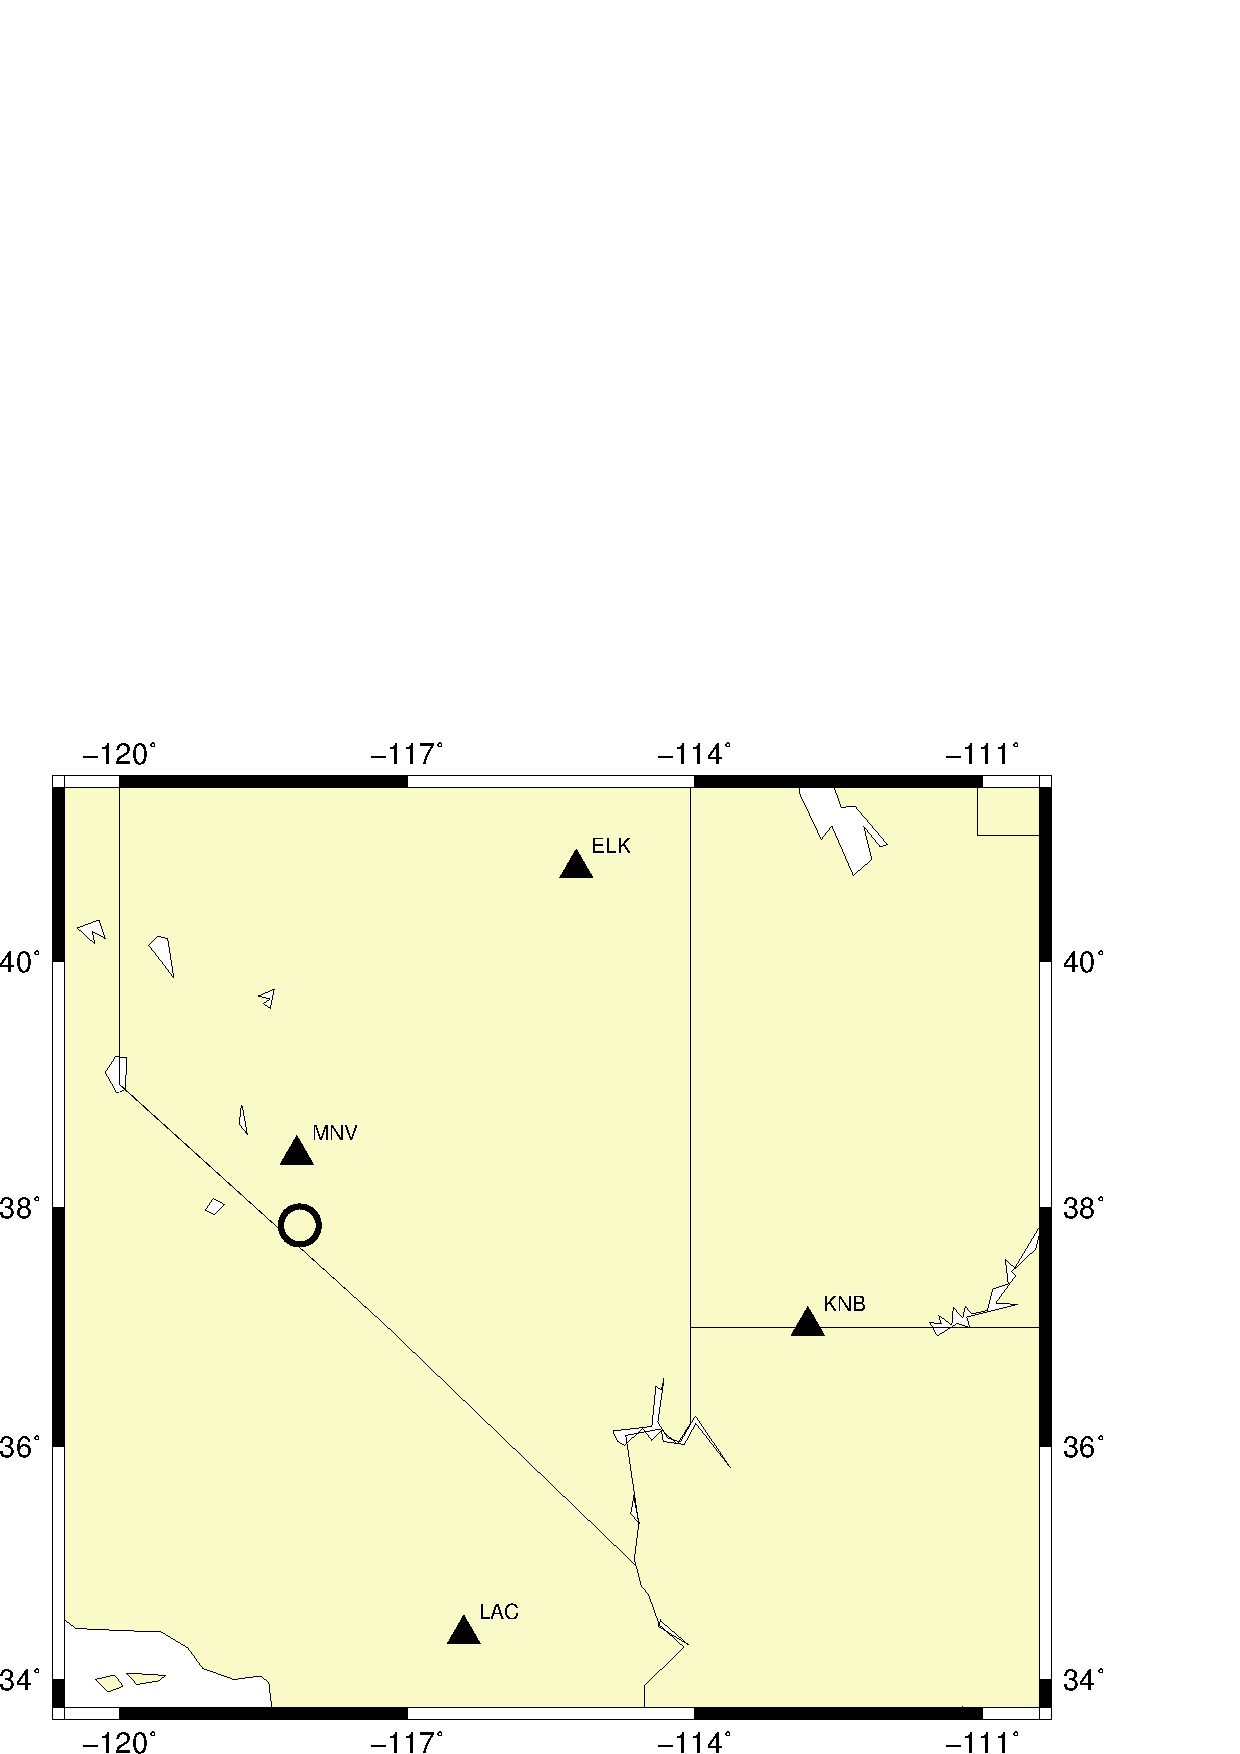
\includegraphics[width=0.7\textwidth]{map}
\caption{map绘制地震、台站分布图}
\label{fig:map}
\end{figure}

\SACTitle{头段数据}
台站纬度(stla)以及经度(stlo)必须在头段中被定义。如果事件纬度(evla)以及经度(evlo)被定义则其会被包含在地图中。如果这个命令在执行BBFK之后执行,MAP将沿着反方位角方向绘制大圆弧路径。
这个版本的MAP是基于4.0版本的Generic Mapping Tools,要执行这个命令,你需要将GMT4.0安装在你的机器上并保证可执行文件位于路径中。

每个MAP命令的结果将写入当前目录下一个称为gmt.csh的脚本中。用户可以修改这个文件以利用更多SAC未利用的选项。默认单位是inch,当然可以在脚本中修改。

在使用pscoast绘制海岸线时,SAC采用了-Dl选项,其中l代表低精度的海岸线数据。用户
可以在脚本中修改使用更高精度的海岸线数据。

该脚本采用的shell是csh,其很容易改成bash脚本。

MAP命令的结果将自动被显示。用于显示的默认程序是gs(ghostscript)。用户可以通过设置环境变量SACPSVIEWER选择其他显示工具。\\
在csh下可以这样设置:
\begin{minted}{console}
setenv SACPSVIEWER "gs -sDEVICE=x11 -q -dNOPROMPT -dTTYPAUSE"
\end{minted}

在bash下可以这样设置:
\begin{minted}{console}
export SACPSVIEWER="gs -sDEVICE=x11 -q -dNOPROMPT -dTTYPAUSE"
\end{minted}

\input{./commands/markptp}
\input{./commands/marktimes}
\input{./commands/markvalue}
\input{./commands/mathop}
\input{./commands/merge}
\input{./commands/message}
\input{./commands/mtw}
\input{./commands/mul}
\input{./commands/mulf}
\input{./commands/mulomega}
\SACCMD{news}
\label{cmd:news}

\SACTitle{概要}
终端显示关于SAC的一些信息

\SACTitle{语法}
\begin{SACSTX}
NEWS
\end{SACSTX}

\SACTitle{说明}
其实质就是将文件~\verb+$SACHOME/aux/news+~的内容显示到终端。

\input{./commands/null}
\input{./commands/oapf}
\input{./commands/ohpf}
\input{./commands/pause}
\input{./commands/picks}
\input{./commands/plabel}
\input{./commands/plot}
\input{./commands/plot1}
\input{./commands/plot2}
\input{./commands/plotalpha}
\SACCMD{plotc}
\label{cmd:plotc}

\SACTitle{概要}
使用光标标注SAC图形和创建图件

\SACTitle{语法}
\begin{SACSTX}
P!LOT!C [R!EPLAY!|C!REATE!] [F!ILE!|M!ACRO! filename] [B!ORDER! ON|OFF]
\end{SACSTX}

\SACTitle{输入}
\begin{description}
\item [REPLAY] 重新显示或绘制一个已经存在的文件或宏,关于文件和宏的区别见下
\item [CREATE] 创建一个新的文件或宏
\item [FILE filename] 重新显示或创建一个文件。如果省略文件名则使用上一个文件
\item [MACRO filename] 重新显示或创建一个宏
\item [BORDER ON|OFF] 打开/关闭图形的边界
\end{description}

\SACTitle{缺省值}
\begin{SACDFT}
plotc create file out border on
\end{SACDFT}

\SACTitle{说明}
这个命令让你可以注释一个SAC绘图或者创建一个用于会议或报告的图件。简单的说就是一个简单的``画图''软件。你需要一个具有光标的图形设备。你可以通过在终端屏幕上放置一个目标(比如圆、方)或者文本创建一个图件。光标的位置决定了目标绘制的位置,敲入的字符决定了要绘制哪个目标。目标包括圆、矩形、多边形、线、箭头、弧,还有多种放置文本的方法。

这个命令绘制出的图可以直接截图利用,绘制过程中用到的所有命令将作为输出文件输出。这个命令有两种输出文件格式:简单文件或宏文件。两者都是字符数字型文件,可以直接用文本编辑器修改。它们包含了PLOTC命令中光标响应的历史以及位置。宏文件一旦被创建,可以用于更多的绘图。其比例和旋转角度均可以修改。简单的PLOTC文件名以``.PCF''为后缀,宏文件名则以``.PCM''为后缀。这使得你可以区分你的目录下的这些文件。

当你创建一个新的文件或宏时,SAC在屏幕上绘制一个矩形,代表你可以绘图的区域,你可以将光标移动到该区域内任何你想放置的位置,并输入代表你想绘制的目标或你想要光标执行的动作所对应的字符。

有两种光标选项类型:动作类和参数设置类。动作类选项将做一些事情(绘制一个矩形,放一些文本),他们如何执行这个操作部分基于当前参数设置选项的值(例如多边形的	边数,文本大小等)。这个区别与SAC自己的操作命令和参数设定命令相同。下面会列出动作和参数设定选项。

当你重新显示一个文件或者宏时,图形在终端屏幕上将会重新绘制,光标也将打开。你可以像你当初创建这个文件一样向其中加入目标。当你完成创建图件之后你可以将其发送到不同的图形设备,使用~\nameref{cmd:begindevices}命令临时关闭终端屏幕打开其他图形设备(比如sgf),然后重新显示这个文件。

为了注释一个SAC绘图,要执行~\nameref{cmd:vspace}命令设置正确的横纵比,然后执行~\nameref{beginframe}命令关闭自动刷新,执行需要的SAC绘图命令,执行~\nameref{cmd:plotc}命令(创建或者重新显示),然后执行~\nameref{cmd:endframe}命令恢复自动刷新。

\SACTitle{示例}
下面的例子展示了如何使用PLOTC命令给一个SAC标准绘图添加注释:
\begin{SACCode}
SAC> fg impulse npts 1024                      //生成文件
SAC> lp c2 n 7 c 0.2 t 0.25 a 10               //低通滤波
SAC> fft
 DC level after DFT is 1
SAC> axes only l b                             //左和下坐标轴设置
SAC> ticks only l b
SAC> border off
SAC> fileid off
SAC> qdp off
SAC> vspace 0.75                              //修改图形尺寸
SAC> beginframe                               //开始绘图
SAC> psp am linlin                            //绘图
SAC> plotc create file bandpass               //开始在图上做注释
...用光标和键盘进行各种操作...
SAC> endframe
\end{SACCode}

\nameref{cmd:plotsp}用于绘制滤波响应曲线以及两个轴,\nameref{cmd:plotc}用于
交互式地添加注释。\nameref{cmd:vspace}命令限制了图形中纵横比为3:4的区域为绘图区域。
这个对于之后将输出发送到具有纵横比3:4的SGF设备来说很有必要。在这之后你将
有一个叫做``BANDPASS.PCF''的文件,其中包很了这个图形的注释信息。

为了将注释写入SGF文件:
\begin{SACCode}
SAC> begindevices sgf                       //打开sgf设备
SAC> beginframe
SAC> plotsp
SAC> plotc replay                           //重新绘制上一注释图
SAC> endframe
\end{SACCode}
这样一个包含注释绘图的SGF文件就建立了。

\SACTitle{注意}
\begin{enumerate}
\item 只有当设置正方形视窗(VSPACE 1.0)时绘制的圆形和扇形才是正确的,否则只能产生一个椭圆,其纵横比等于视窗的纵横比。
\item 除文本之外的所有操作码都按比例适应图形窗口。
\end{enumerate}
文本尺寸并不是当前标度的。当你生成一个图像并想要将文本放在一个矩形或圆中时会产生一个问题。在这种情况下,图形窗口必须与输出页具有相同的尺寸,以避免图形的偏差。这可以通过使用WINDOW命令设置窗的水平(x)尺寸为0.75,垂直(y)尺寸为0.69。
例如: WINDOW 1 X 0.05 0.80 Y 0.05 0.74。这个命令必须在窗口被创建之前执行。(即在BEGINWINDOW或BEGINDEVICES之前)

\SACTitle{相关命令}
\nameref{cmd:vspace}、\nameref{cmd:begindevices}、\nameref{cmd:beginframe}、\nameref{cmd:endframe}

\begin{table}[!ht]
\centering
\ttfamily
\small
\caption{plotc命令表}
\begin{tabular}{p{1cm}p{10cm}}
	\toprule
	字符	& 	含义	\\
	\midrule
	A		&	绘制一条到ORIGIN到CURSOR的箭头	\\
	B		&	在绘图区周围绘制边界的tick标记  \\
	C		&	绘制一个圆心在ORIGIN,且经过CURSOR的圆	\\
	D		&	从replay文件中删除最后一个动作选项	\\
	G		&	设置ORIGIN,并将其全局化	\\
	L		& 	绘制一条从ORIGIN到CURSOR的线	\\
	M		&	在CURSOR处插入一个宏文件(输入宏文件名,比例因子和旋转角。
                若没有指定,则使用上一次的值,默认是OUT,1.0,0)\\
	O		&	设置ORIGIN为CURSOR		\\
	N		&	绘制一个中心在ORIGIN,一个顶点位于CURSOR的n边形 \\
	Q		&	退出PLOTC	\\
	R		&	绘制对脚位于ORIGIN和CURSOR的长方形	\\
	S		&	绘制一个圆心位于ORIGIN的扇形(用光标的移动来
                指定扇形的角度,键入S来绘制一个小于180度的扇形,或者键入C绘制它的补集)\\
	T		&	在CURSOR处放置一行文本,文本以回车键结束	\\
	U		&	在CURSOR处放置多行文本,文本以空白行结束	\\
	\bottomrule
\end{tabular}
\end{table}
\SACTitle{关于PLOTC命令表的说明}
\begin{itemize}
\item CURSOR表示当前光标位置
\item ORIGIN一般为上次光标的位置
\item G选项强制ORIGIN固定
\item O选项再次允许ORIGIN移动
\item Q选项不自动拷贝至文件,但是可以通过文本编辑器直接加入
\end{itemize}
如果SAC在replay模式没有在文件中看到Q选项,则其在显示文件内容之后回到光标
模式,这使得你可以在文件结束之后继续增加更多的选项。如果SAC在文件中看到
Q选项,则显示其内容并退出。文件中以星号开头的行为注释行。
PLOTC还有一些更复杂的选项,但是运行起来好像有点问题,有兴趣的可以试试
``help plotctable''。

\input{./commands/plotdy}
\input{./commands/plotpk}
\input{./commands/plotpm}
\input{./commands/plotsp}
\input{./commands/plotxy}
\input{./commands/print}
\input{./commands/printhelp}
\input{./commands/production}
\input{./commands/qdp}
\input{./commands/quantize}
\input{./commands/quit}
\input{./commands/quitsub}
\input{./commands/read}
\input{./commands/readbbf}
\input{./commands/readerr}
\input{./commands/readhdr}
\SACCMD{readsp}
\label{cmd:readsp}

\SACTitle{概要}
读取~\nameref{cmd:writesp}和~\nameref{spe:writespe}写的谱文件

\SACTitle{语法}
\begin{SACSTX}
R!EAD!SP [AMPH|RLIM|SPE] [filelist]
\end{SACSTX}

\SACTitle{输入}
\begin{description}
\item [RLIM]  读入实部和虚部分量
\item [AMPH]  读入振幅和相位分量
\item [SPE] 读取谱估计子程序文件,这个数据被从功率转换为振幅,相位分量设置为0
\item [filelist] SAC二进制数据文件列表
\end{description}

\SACTitle{缺省值}
\begin{SACDFT}
READSP AMPH
\end{SACDFT}

\SACTitle{说明}
\nameref{cmd:writesp}命令将每个谱数据分量作为一个单独的文件写入磁盘,
你可以分别处理每个分量。这个命令让你能从两个分量重建谱数据,参见~\nameref{cmd:writesp}。
SPE选项允许你读取并转换由\nameref{spec:writespe}写出的谱文件格式。
这也使你可以使用~\nameref{cmd:mulomega}和~\nameref{cmd:divomega}命令。

\SACTitle{相关命令}
\nameref{cmd:writesp}

\input{./commands/readtable}
\input{./commands/report}
\input{./commands/reverse}
\section{去毛刺}
相关命令:\nameref{cmd:rglitches}

地震仪器偶尔会出现问题,导致连续地震数据流中出现尖锋或者数据丢失。
这些所谓的毛刺,肉眼很容易识别,但是在进行数据分析中却很容易被误认为是地震信号,
因而需要在数据分析之前将毛刺去除。数据的毛刺在模拟地震记录中很常见,现在的数字
地震记录中则很少见到。rglitches命令可以在某种程序上去除地震信号中的毛刺。

rglitches的效果可以从图~\ref{fig:deglitches}~中直观地看到。

\begin{figure}[H]
\centering
\includegraphics[width=0.75\textwidth]{rglitches}
\caption[地震波形去毛刺]{地震波形去毛刺。上图为包含glitches的地震信号,下图为去除
rglitches后的地震信号。}
\label{fig:deglitches}
\end{figure}

\input{./commands/rmean}
\input{./commands/rms}
\input{./commands/rotate}
\input{./commands/rq}
\SACCMD{rtrend}
\label{cmd:rtrend}

\SACTitle{概要}
去除线性趋势
\footnote{101.6和101.6a的rtrend命令存在Bug,详情参考\url{http://seisman.info/sac-bugs.html}}

\SACTitle{语法}
\begin{SACSTX}
RTR!END! [Q!UIET!|!V!ERBOSE]
\end{SACSTX}

\SACTitle{输入}
\begin{description}
\item [QUIET] 不显示线性拟合信息
\item [VERBOSE] 终端显示线性拟合信息
\end{description}

\SACTitle{缺省值}
\begin{SACDFT}
rtrend quiet
\end{SACDFT}

\SACTitle{说明}
该命令利用最小二乘方法将数据拟合成一条直线,然后从数据中减去该直线所表征的线性趋势。
数据可以是不等间隔的。

若有$n$个数据$(x_i,y_i)$,利用最小二乘法拟合直线$y=ax+b$。其中斜率为
\[
    a = \frac{n\sum x_i y_i - \sum x_i \sum y_i}
    {n\sum x_i^2 - (\sum x_i)^2}
\]

Y轴截距为
\[
    b = \frac{\sum x_i^2 \sum y_i - \sum x_i \sum x_i y_i}
    {n\sum x_i^2 - (\sum x_i)^2}
\]

内存中最后一个文件的线性拟合参数将会写入到如下黑板变量中:
\begin{itemize}
\item RTR\_SLP 直线斜率
\item RTR\_YINT 直线的Y截距
\item RTR\_SDSLP 斜率的标准差
\item RTR\_SDYINT Y截距的标准差
\item RTR\_SDDTA 数据的标准差
\item RTR\_CORRCF 数据和拟合结果的相关系数
\end{itemize}

\SACTitle{错误消息}
\begin{itemize}
\item[-]1301: 未读入数据文件
\item[-]1307: 对谱文件的非法操作
\end{itemize}

\SACTitle{头段变量改变}
depmin、depmax、depmin

\input{./commands/saveimg}
\input{./commands/setbb}
\input{./commands/setdevice}
\input{./commands/setmacro}
\input{./commands/sgf}
\input{./commands/smooth}
\input{./commands/sonogram}
\input{./commands/sort}
\input{./commands/spectrogram}
\input{./commands/sqr}
\input{./commands/sqrt}
\input{./commands/stretch}
\input{./commands/sub}
\input{./commands/subf}
\input{./commands/symbol}
\input{./commands/synchronize}
\SACCMD{systemcommand}
\label{cmd:systemcommand}

\SACTitle{概要}
在SAC内部执行系统命令

\SACTitle{语法}
\begin{SACSTX}
S!YSTEM!C!OMMAND! command [ options ]
\end{SACSTX}

\SACTitle{输入}
\begin{description}
\item [command] 系统命令名
\item [options] 命令需要的选项
\end{description}

\SACTitle{说明}
在SAC中是可以执行大部分系统命令的,比如常见的~\verb+ls+、\verb+cp+~等。

但是某些命令无法直接在SAC中执行,比如用于查看PS文件的gs命令会首先被SAC解释为
\nameref{cmd:grayscale}的简写,故而在SAC中无法直接调用gs命令。

另一个经常使用但无法直接调用的命令是~\verb+rm+。由于~\nameref{cmd:read}~命令
可以被简写为~\verb+r+,在读入文件时键入~\verb+r *.SAC+~很可能会一时手误
敲成~\verb+rm *.SAC+,为了避免类似的误操作,故而在SAC中禁止直接调用
~\verb+rm+~命令。

当需要在SAC内部执行删除命令时,则需要使用~\nameref{cmd:systemcommand}~调用系统命令。

\SACTitle{示例}
调用系统命令删除某些SAC文件:
\begin{SACCode}
SAC> rm junks
 ERROR 1106: Not a valid SAC command.
SAC> sc rm junks
\end{SACCode}

\SACCMD{taper}
\label{cmd:taper}

\SACTitle{概要}
对数据两端应用对称的taper函数,使得数据两端平滑地衰减到零

\SACTitle{语法}
\begin{SACSTX}
TAPER [T!YPE! HAN!NING!|HAM!MING!|C!OSINE!] [W!IDTH! v]
\end{SACSTX}

\SACTitle{输入}
\begin{description}
\item [TYPE HANNING|HAMMIN|COSINE] 应用Hanning、Hamming、余弦衰减窗
\item [WIDTH v] 设置衰减窗的宽度占数据总点数(npts)的比值为v,v取值在0.0和0.5之间
\end{description}

\SACTitle{缺省值}
\begin{SACDFT}
taper type hanning width 0.05
\end{SACDFT}

\SACTitle{说明}
taper函数是在0和1之间取值的单调函数,若将其对称地施加于数据的首尾两端,则可实现
数据的``尖灭''。

taper函数共计$npts*v$个点,第一个点值为0,最后一个点的值为1,将此函数的每个点依次
于数据的第1至$npts*v$个点相乘,使得数据数据的首端从0开始光滑地增加到其原始值。
数据的末端完全类似,此时数据由其原始值不断光滑地减小到0。

taper命令的通用形式为
\[
    Data(j) = Data(j)*(F_0 - F_1\cos(\omega(j-1)))
\]
此公式应用于数据的首端,另一个完全对称的数据用于数据的尾端。

表~\ref{table:taper-functions}~定义了不同的衰减函数的参数,其中N为衰减窗的宽度,即$npts*v$。
\begin{table}[ht]
\centering
\caption{taper衰减函数参数一览}
\label{table:taper-functions}
\begin{tabular}{llll}
\toprule
类型 & $\omega$ & $F_0$	& $F_1$	\\
\midrule
HANNING	&	$\frac{\pi}{N}$	&	0.50	&	0.50	\\
HAMMING	&	$\frac{\pi}{N}$	&	0.54	&	0.46	\\
COSINE	&	$\frac{\pi}{2N}$	&	1.00	&	1.00	\\
\bottomrule
\end{tabular}
\end{table}

图~\ref{fig:taper-functions}~给出了不同taper衰减函数的曲线图,图中可以看出,HAMMING
窗实际上并没有完全实现尖灭。
\begin{figure}[!ht]
\centering
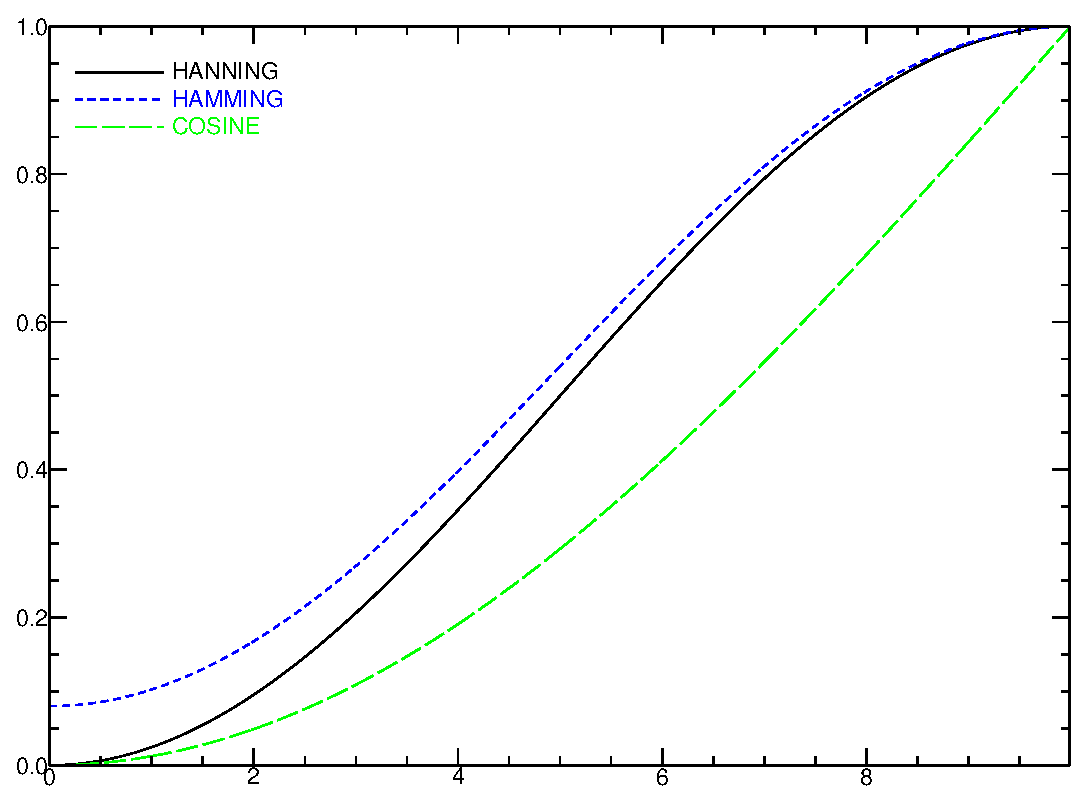
\includegraphics[width=0.8\textwidth]{taper-functions}
\caption{taper衰减函数曲线}
\label{fig:taper-functions}
\end{figure}

\SACTitle{错误消息}
\begin{itemize}
\item[-]1301: 未读入数据文件
\item[-]1306: 对不等间隔文件的非法操作
\end{itemize}

\SACTitle{头段变量}
depmin、depmax、depmen

\input{./commands/ticks}
\input{./commands/title}
\SACCMD{trace}
\label{cmd:trace}

\SACTitle{概要}
追踪黑板变量和头段变量

\SACTitle{语法}
\begin{SACSTX}
TRACE [ON|OFF] name [name ...]
\end{SACSTX}

\SACTitle{输入}
\begin{description}
\item [ON] 打开变量追踪选项
\item [OFF] 关闭变量追踪选项
\item [name] 要追踪的黑板变量或/和头段变量名。对于头段变量,其格式为\verb+filename,hdrname+,
    其中filename是要追踪的SAC文件名或文件号,hdrname是SAC头段变量名。
\end{description}

\SACTitle{缺省值}
\begin{SACDFT}
trace on
\end{SACDFT}

\SACTitle{说明}
该命令用于在SAC执行过程中追踪SAC黑板变量或/和头段变量的值,主要用于调试大型或复杂的宏文件。
当变量追踪选项被打开时,将显示变量的当前值。若变量追踪选项处于打开状态,则每次执行命令时将
对变量值进行检查,若变量的值发生改变则将其新值打印到终端。当变量追踪选项被关闭时,也会显示
变量的当前值。

\SACTitle{示例}
追踪黑板变量TEMP1和文件MYFILE的头段变量T0:
\begin{SACCode}
SAC> trace on temp1 myfile,t0
  TRACE  (on) TEMP1 = 1.45623
  TRACE  (on) MYFILE,T0 = UNDEFINED
\end{SACCode}

在执行命令时,SAC会检查变量值是否发生改变。若发生改变则将相关信息显示出来。假设在完成一些计算之后
改变了TEMP1,并定义了T0的值,则SAC将显示如下信息:
\begin{SACCode}
  TRACE (mod) TEMP1 = 2.34293
  TRACE (mod) MYFILE,T0 = 10.3451
\end{SACCode}

稍后的处理中TEMP1可能再次改变:
\begin{SACCode}
  TRACE (mod) TEMP1 = 1.93242
\end{SACCode}

当跟踪选项被关闭时,SAC最后一次显示变量当前值:
\begin{SACCode}
SAC> trace off temp1 myfile,t0
  TRACE (off) TEMP1 = 1.93242
  TRACE (off) MYFILE,T0 = 10.3451
\end{SACCode}

\SACCMD{transcript}
\label{cmd:transcript}

\SACTitle{概要}
控制输出到副本文件

\SACTitle{语法}
\begin{SACSTX}
TRANSCRIPT [OPEN|CREATE|CLOSE|CHANGE|WRITE|HISTORY] [FILE filename]
    [CONTENTS ALL|ERRORS|WARNINGS|OUTPUT|COMMANDS|MACROS|PROCESSED]
    [MESSAGE text]
\end{SACSTX}

\SACTitle{输入}
\begin{description}
\item [OPEN] 打开副本文件,并在已存在的文件底部添加副本
\item [CREATE] 创建一个新的副本文件
\item [CLOSE] 关闭一个已经打开的副本文件
\item [CHANGE] 改变一个已经打开的副本文件的内容
\item [WRITE] 写信息到一个副本文件,不改变其状态或内容
\item [HISTORY FILE filename] 将命令行历史保存到文件
\item [FILE filename] 定义副本文件的名字
\item [MESSAGE text] 向副本文件中写入文本。这个信息可以用于指定正在进行的进程或指定正在
    处理的不同事件,在两次执行这个命令的过程中这个信息不保存。
\item [CONTENTS ALL] 定义副本文件的内容为全部输入输出的信息。
\item [CONTENTS list] 定义副本文件的内容,即包含在文件中的输入输出的类型表
\end{description}
其中list可以取:
\begin{itemize}
\item ERRORS : 执行命令期间产生的错误消息
\item WARNINGS : 执行命令期间产生的警告消息
\item OUTPUT : 执行命令期间的输出消息
\item COMMANDS : 终端输出的原始命令
\item MACROS : 宏文件中出现的原始命令
\item PROCESSED : 经终端或宏处理之后的命令
\end{itemize}

\SACTitle{缺省值}
\begin{SACDFT}
transcript open file transcript contents all
\end{SACDFT}

\SACTitle{说明}
副本文件用于记录SAC执行的结果。其可以是一个完整或部分副本,可以包含一次或多次执行
的结果。你可以同时拥有5个活动的副本文件,每个文件用于追踪不同的方面。
其中的一个用途是记录终端输入的命令然后用于一个宏文件中,如下例所示。

\SACTitle{示例}
为了创建一个新的副本文件,文件名为MYTRAN,包含了除已处理命令之外的其他全部类型:
\begin{SACCode}
SAC> transcript create file mytran cont err warn out com macros
\end{SACCode}

如果之后不想把宏命令送入这个文件,你可以使用CHANGE选项:
\begin{SACCode}
SAC> transcript change file mytran contents errors warnings output commands
\end{SACCode}

为了定义一个名为MYRECORD的副本文件,其记录了终端输入的命令:
\begin{SACCode}
SAC> transcript create file myrecord contents commands
\end{SACCode}

以后,经过适当的编辑,这个文件可以用作宏命令文件,去自动执行相同的一组命令。在最后的例子中假设你需要彻夜处理许多事件。你可以设置每个事件一个副本文件(用不同的副本文件名)去记录处理的结果。另外你可以将处理所有事件得到的任何错误消息保存到一个副本文件中:
\begin{SACCode}
SAC> transcript open file errortran contents errors
SAC> transcript write message 'processing event 1'
\end{SACCode}

这些命令将放在处理每个事件的宏文件中,它假设事件名作为第一个参数带入宏。使用打开选项,
运行信息和出错信息将添加到文件的后面,第二天检查一下这个出错信息副本文件,就可以快速
查阅在处理期间是否出现了错误。

为了将保存一个命令行副本,以记录SAC当前和将来要运行的命令:
\begin{SACCode}
SCA> transcript history file .sachist
\end{SACCode}
这就在当前目录创建并写入了一个副本文件``./.sachist''。任何储存在那里的文件将被载入命令历史中。
如果这个命令位于你的启动初始化宏文件中,则每次你运行SAC时将在当前目录产生一个单独的命令行历史。
在一个新执行的SAC中,上下键将浏览完整的命令历史,你可以修改以前输入的命令并再次执行它,
如果你没有在SAC内或初始化宏文件中输入这个命令,则命令行历史将自动保存到~\verb+~/.sac_history+

\SACCMD{transfer}
\label{cmd:transfer}

\SACTitle{概要}
去仪器响应,并加上其他仪器响应

\SACTitle{语法}
\begin{SACSTX}
TRANS!FER! [FROM type [options]] [TO type [options]]
    [FREQ!LIMITS! f1 f2 f3 f4] [PREWH!ITENING! ON|OFF|n]
\end{SACSTX}

\SACTitle{输入}
\begin{itemize}
\item FROM type : 要去除的仪器响应类型;
\item TO type : 要加入的仪器响应类型;
\item FREQLIMITS f1 f2 f3 f4:压制大于f4以及低于f1的频段;
\item PREWHITENING ON|OFF|n:预白化处理。
\end{itemize}

\SACTitle{缺省值}
\begin{SACDFT}
trans from none to none
\end{SACDFT}

\SACTitle{说明}
关于仪器响应的详细说明,请参考附录中的``\nameref{chap:resp}''一章。

transfer命令的作用是从波形中去除仪器响应,如果需要,也可以再卷积上某类型的
仪器响应。\verb+from+给出了波形当前的仪器响应,也就是要去除的仪器响应。
\verb+to+给出了要卷积上的仪器响应。

freqlimits用于在去除仪器响应的时候对波形的低频和高频部分进行压制。通常这一选项
是很重要的。这是因为所有的地震仪在零频率处都具有零响应。当做反卷积但不卷积其他
响应的时候(即\verb+to none+),就有必要修改超低频率处的响应以防止频率域除0。
在高频区域,信噪比通常很低,因而有必要对其响应进行抑制。
freqlimites包含了低通和高通的尖灭函数(taper),可以实现高频和低频的有效压制。
四个频率满足f1<f2<f3<f4,尖灭函数在f2和f3间为1,在f1以下和f4以上为0。频率f1和
f2确定了高通滤波器的特性,频率f3和f4指定了低通滤波器的特性。
f1与f2之间以及f3与f4之间分别为余弦波的四分之一个周期。

如果你想要一个低通滤波器但在低频处不滤波,一种方法是设置f1=-2和f2=-1;
如果你想要一个高通滤波器但在高频处不滤波,对于Nyquist频率为0.5,设置f3=10和f4=20。

注意:由于滤波器还有零相位,因而其是非因果。如果数据点数npts不为2的指数幂次,
会导致在频段(f1,f4)之外振幅不为0。如果想要数据点数为2的幂次方个,可以参考SAC中的CUT命令。

\verb+prewhitening+用于控制数据的预白化。预白化可以将输入时间序列在变换到
频率域之前,进行谱的平化。这会减小谱值的动态范围,并提高数据在高频的计算精度。
参见\nameref{cmd:whiten}命令。打开预白化选项,会在谱操作之前在频率域进行谱白化,
并在谱操作后在时间域做谱白化的补偿,也可以设置预白化选项的阶数。默认情况下,
预白化选项是关闭的,阶数为n=6。

transfer中的from和to后,接具体的仪器类型。在SAC中,可以用5种方式来指定要使用的
仪器类型,即内置仪器类型、特殊内置仪器类型、RESP文件、PZ文件和FAP文件。

\subsubsection{内置仪器类型}
SAC内置了一堆标准仪器的响应函数,可以在命令中直接使用。但是因为日常中其实很少
使用这些内置仪器类型,或者只是用到很少的几个,故而把这些仪器类型放在附录的表
\ref{table:instrument-type}中。

为了从数据中去除LLL宽频带仪器响应,并卷积上SRO仪器响应,且对频带做尖灭及预白化:
\begin{SACCode}
SAC> read abc.z
SAC> rmean; rtr; taper
SAC> trans from lll to sro freq .02 .05 1. 2. prew 2
\end{SACCode}

某些内置仪器类型,还有子类型(subtype)。
当前仪器为RSTN类型的nykm.z子类型,为了从波形数据中去除该仪器响应,并卷积上DSS仪器响应:
\begin{SACCode}
SAC> read nykm.z
SAC> rmean; rtr; taper
SAC> trans from rstn subtype nykm.z to dss prew off
\end{SACCode}

\subsubsection{特殊仪器类型}
SAC中定义了三个特殊的仪器类型,即\verb+none+、\verb+vel+和\verb+acc+,分别表示
位移、速度和加速度。

\begin{itemize}
\item 若使用\verb+to none+,则表示在去除原有仪器响应后,再卷积上none对应的仪器响应。
    而none对应的响应函数在全频段内振幅为1,相位为零,即相当于没有卷积新的仪器响应。
    这样会得到位移波形,同时SAC头段变量idep将被设置为DISPLACEMENT。
\item 若使用\verb+to vel+或\verb+to acc+,则将得到速度场或加速度场。
\item 若使用\verb+from none+,则不会去除仪器响应,原始的地震波形数据认定为位移,
    这常用于向合成地震图中加入仪器响应。\verb+from vel+和\verb+from acc+同理。
\end{itemize}

从波形中去除WWSP的仪器响应,得到位移波形:
\begin{SACCode}
SAC> read xyz.z
SAC> rmean; rtr; taper
SAC> transfer from WWSP to none freq 0.05 0.01 5 10
\end{SACCode}

向合成的位移地震图中加入WWSP仪器响应:
\begin{SACCode}
SAC> r syn.z
SAC> transfer from none to WWSP
\end{SACCode}

\subsubsection{RESP文件}
可以直接用\verb+evalresp fname+后接RESP文件名来指定仪器响应:
\begin{SACCode}
SAC> r 2006.253.14.30.24.0000.TA.N11A..LHZ.Q.SAC
SAC> rmean; rtr; taper
SAC> trans from evalresp fname RESP.TA.N11A..LHZ to none freq 0.004 0.007 0.2 0.4
\end{SACCode}

若未使用fname显式指定RESP文件,evalresp选项会从SAC头段区中提取出台网名、台站名、
位置ID、通道名,并尝试在当前工作目录下去寻找文件名为
~``\verb+RESP.<NET>.<STA>.<LOCID>.<CHAN>+''~的RESP响应文件:
\begin{SACCode}
SAC> r 2006.253.14.30.24.0000.TA.N11A..LHZ.Q.SAC
SAC> rtr; taper
SAC> trans from evalresp to none freq 0.004 0.007 0.2 0.4
            // 在当前目录自动寻找文件RESP.TA.N11A..LHZ
\end{SACCode}

一个RESP文件可以包含多个响应函数,既可以是同一仪器在不同时期的响应函数,也可以是
多个台站的响应函数。transfer命令会从波形中的头段区提取出相关信息,并从RESP文件
中找出全部信息都匹配的响应函数。
\begin{SACCode}
SAC> r 2013.144.05.40.09.0195.IU.COLA.00.BHZ.M.SAC
SAC> rmean; rtr; taper
SAC> transfer from evalresp fname RESP.ALL to none freq 0.1 0.2 5 10
        // RESP.ALL中包含了多个台站的响应函数
\end{SACCode}

也可以通过给evalresp选项指定额外的选项和参数来覆盖SAC文件中对应的头段变量,
这些可能的选项包括:STATION、CHANNEL、NETWORK、DATE、TIME、LOCID。
每个选项都必须有一个合适的值,若DATE在SAC头段中为设定且在选项中未指定,
则使用当前系统日期,TIME同理。
若NETWORK未指定,则默认使用任意台站名;若LOCID未指定,则默认使用任意LOCID。

从文件中去除仪器响应,并卷积上COLB台站的仪器响应:
\begin{SACCode}
SAC> r 2013.144.05.40.09.0195.IU.COLA.00.BHZ.M.SAC
SAC> rtr; taper
SAC> trans from evalresp to evalresp station COLB
    // 当前目录下必须有COLA和COLB两个台站的仪器响应文件
    // 该命令会去除RESP.IU.COLA.00.BHZ的响应函数
    // 并卷积RESP.IU.COLB.00.BHZ的响应函数
    // PS: COLB台站是我瞎编的
\end{SACCode}

为了显示IU台网COL台站BHZ通道,1992年01月02日16:42:05的仪器响应:
\begin{SACCode}
SAC> fg impulse npts 16384 delta .05 begin 0.
SAC> trans to evalresp sta COL cha BHZ net IU date 1992/2 time 16:42:05
SAC> fft
SAC> psp am
\end{SACCode}

上面给了RESP文件的一堆例子,日常输出处理时最常用的还是直接用fname指定RESP响应
文件。

\subsubsection{PZ文件}
可以使用\verb+polezero subtype+后接PZ文件的方式来指定响应文件:
\begin{SACCode}
SAC> r XXX.Z
SAC> rmean; rtr; taper
SAC> trans from polezero subtype XXX.PZ to WWSP
\end{SACCode}

PZ文件中可以包括多个台站的PZ文件。假设用rdseed在当前目录产生了多个台站的PZ文件,
并将所有PZ文件合并得到一个新的PZ文件event.pz。下面的例子将读入全部BH*波形文件,
经仪器响应校正并覆盖原文件:
\begin{SACCode}
SAC> r *BH*SAC          // 读入全部数据
SAC> rtr
SAC> taper
SAC> trans from polezero s event.pz freq 0.05 0.1 10.0 15.0
SAC> w over
\end{SACCode}

虽然没有进过验证,但根据经验做如下合理猜测:当把多个PZ文件合并成一个总PZ文件时,
PZ文件中的注释行就很重要了,transfer命令会从中提取相关信息与波形的头段信息进行
匹配,以找到合适的响应函数。因为对每个波形,都需要到总PZ文件中寻找匹配的响应
函数,所以上例所示的方法,虽然可以很简单地批量去仪器响应,但效率可能不高,尤其
是当台站数目很多、PZ文件较大的时候。

\subsubsection{FAP文件}
FAP文件不太常用,这里仅举一例。

假设有fapfile文件~\verb+fap.n11a.lhz_0.006-0.2+,其名字表示频率段为0.006 Hz到0.2 Hz,
要从波形~\verb+2006.253.14.30.24.0000.TA.N11A..LHZ.Q.SAC+中移除该仪器响应:
\begin{SACCode}
SAC> r 2006.253.14.30.24.0000.TA.N11A..LHZ.Q.SAC
SAC> rtr
SAC> taper
SAC> trans from fap s fap.n11a.lhz_0.006-0.2 to none freq 0.004 0.006 0.1 0.2
SAC> mul 1.0e9
\end{SACCode}

\section{震相理论到时}
震相理论到时的计算是地震学的基础,具体的原理涉及到一大堆公式,感兴趣的读者可以阅读相关文献。

日常工作中经常需要识别震相、将波形按理论到时排序或迭加、计算震相到时残差等等,这些都需要用到震相理论到时,将震相理论到时写入到SAC文件的头段中,可以使得后期处理更加简单。

SAC头段中可以用于保存震相到时信息的头段包括:a、f以及tn(n=0-9),ka、kf和ktn中则用于保存相应的震相名信息。

给SAC文件标记理论到时有三种方法,下面一一介绍。

\subsection{手动标记}
最直观的办法是根据SAC文件中的震源深度和震中距信息用某些程序计算出理论到时,然后用~\nameref{cmd:chnhdr}~命令手动将到时信息写入到SAC头段中。

\begin{SACCode}
SAC> dg sub teleseis nykl.z     // 以nykl.z为例
SAC> lh evdp gcarc         // 查看震源深度和震中距

  FILE: /opt/sac/aux/datagen/teleseis/nykl.z - 1
   ------------------------------------------

     evdp = 0.000000e+00
    gcarc = 3.841450e+01
// 利用某程序计算得到ak135模型下,P波走时为443.14秒,S波走时为799.05秒
// 若SAC文件的参考时间为发震时刻,则
SAC> ch t0 443.14 t1 799.05 kt0 P kt1 S
SAC> lh t0 kt0 t1 kt1

    FILE: /opt/sac/aux/datagen/teleseis/nykl.z - 1
    ------------------------------------------

     t0 = 4.431400e+02
    kt0 = P
     t1 = 7.990500e+02
    kt1 = S
\end{SACCode}

该方法很直接也很基础, 其缺点也很明显,那就是麻烦。

\subsection{traveltime命令}
\nameref{cmd:traveltime}是SAC提供的一个命令,用于计算iasp91或者ak135地球模型下的震相理论走时,并自动将震相到时信息保存到SAC头段变量中。

\begin{SACCode}
SAC> dg sub teleseis nykl.z
SAC> traveltime model iasp91 picks 3 phase P S
traveltime: depth: 0.000000 km
SAC> lh t3 kt3 t4 kt4

  FILE: /opt/sac/aux/datagen/teleseis/nykl.z - 1
   ------------------------------------------

         t3 = 4.430530e+02
        kt3 = P
         t4 = 7.999642e+02
        kt4 = S
\end{SACCode}

该命令会将震相P、S的理论到时依次写入头段变量t3、t4中,并在相应的K头段中写入震相名信息。

该方法的优点在于是SAC内置命令,使用起来也很简单,缺点在于只支持两种地球速度模型。

\subsection{taup\_setsac命令}
\verb+taup_setsac+~是taup软件提供的用于计算震相理论到时的独立于SAC的外部命令。

\begin{minted}{console}
$$ taup_setsac -mod prem -ph P-6,S-7 -evdpkm *.SAC
\end{minted}

该命令会根据SAC文件中的震中距和震源深度信息,计算P和S震相在PREM模型下的理论走时,并写入到SAC头段t6和t7中,同时向kt6和kt7中写入震相名称。

该方法的优点在于支持多种地球标准模型以及自定义模型。

\input{./commands/tsize}
\input{./commands/unsetbb}
\input{./commands/unwrap}
\SACCMD{vspace}
\label{cmd:vspace}

\SACTitle{概要}
改变图形的最大尺寸和形状

\SACTitle{语法}
\begin{SACSTX}
VSP!ACE! FULL|v
\end{SACSTX}

\SACTitle{输入}
\begin{description}
\item [FULL] 使用整个视窗,这是可能的最大屏幕或窗口尺寸
\item [v] 使视窗比y:x为v,具有这个纵横比的最大的区域称为视窗
\end{description}

\SACTitle{缺省值}
\begin{SACDFT}
vspace full
\end{SACDFT}

\SACTitle{说明}
视窗代表了屏幕上可以用于绘图的部分。视窗形状和尺寸在不同图形设备之间有很大的变化。
\begin{enumerate}
\item 尽管在尺寸上有很大不同,许多图形终端都具有0.75的纵横比。
\item SGF文件的纵横比为0.75,其大约是标准的8.5*11英寸纸张的纵横比。
\item  由XWINDOWS或SUNWINDOWS图形设备建立的窗口可以有你想要的任意纵横比
\end{enumerate}

这个命令可以控制纵横比,从而使你能够控制图形的形状缺省绘图是在整个视窗上。
如果确定了一个纵横比,则视窗就是设备上具有这个纵横比的最大区域。

当你使用~\nameref{cmd:plotc}命令在交互设备上建立一张图,并且最终要将它发送到SGF设备上,
这个命令特别有用,在绘制任何图形之前,必须设置纵横比为0.75。这将保证图形在SGF
文件上与在交互设备上相同。如果你要建立一个独立于图形设备的正方形视窗,
则可以简单地设置纵横比为1.0。

\input{./commands/wait}
\SACCMD{whiten}
\label{cmd:whiten}

\SACTitle{概要}
平滑输入的时间序列的频谱

\SACTitle{语法}
\begin{SACSTX}
W!H!IT!EN! n [F!ILTER!D!ESIGN!]
\end{SACSTX}

\SACTitle{输入}
\begin{description}
\item [n]  阶数(极数)。这个数越大,结果数据就越平滑。高阶可以更好的清除一些数据,但是也可能会导致对数据处理过多而丢掉一些重要的数据。默认值为6。
\item [FD] 进行一些类似于filterdesign的命令,使用白化系数,设计一个白化滤波器。详情可以参考filterdesign命令。
\end{description}

\SACTitle{缺省值}
\begin{SACDFT}
whiten 6
\end{SACDFT}

\SACTitle{说明}
对数据中加入白噪声。平滑输入时间序列的频谱。当这个命令在谱分析命令(比如子程序SPE中的命令、transfer或spectrogram)之前执行,其减少了频谱值的动态范围,提供了对地震数据高频操作的精度。

WHITEN可以在SPE子程序内部调用,或者从SAC主程序中调用。SPE中的WHITEN和主程序中的
WHITEN分别有不同的阶数。在主程序中,你可以调用WHITEN 4,下一次在主程序中调用
WHITEN时阶数为4,但是在SPE中调用WHITEN时依然是缺省的6阶,除非你在SPE的命令行中
进行了修改。进一步,SPE中的阶数与SPE COR命令的PREWHITEN选项是一样的
(设置了一个其他的也就设置了)。当然主程序中WHITEN命令与TRANSFER命令中的
PREWHITEN选项也是一样的。

\SACTitle{相关命令}
\nameref{cmd:transfer}

\input{./commands/whpf}
\input{./commands/width}
\input{./commands/wiener}
\input{./commands/wild}
\input{./commands/window}
\input{./commands/write}
\input{./commands/writebbf}
\SACCMD{writehdr}
\label{cmd:writehdr}

\SACTitle{概要}
用内存中文件的头段区覆盖磁盘文字中的头段区

\SACTitle{语法}
\begin{SACSTX}
W!RITE!H!DR!
\end{SACSTX}

\SACTitle{说明}
write命令的over选项可以用内存中头段区和数据区覆盖磁盘文件中的头段区和数据区。
该命令用内存中头段区覆盖磁盘文件中的头段区,数据区不会被覆盖。如果使用了cut命令,
读取数据时将仅读入部分数据,内存中的头段区将会做相应修改以反映cut命令的效果,
但是磁盘中的数据并没有被修改,因而此时不能使用writehdr命令。对被cut的数据
使用WRITEHDR命令将可能导致磁盘中的数据产生类似于平移或截断的效果。

\SACTitle{错误消息}
\begin{itemize}
\item[-]1301: 未读入数据文件
\end{itemize}

\SACTitle{相关命令}
\nameref{cmd:cut}、\nameref{cmd:write}

\input{./commands/writesp}
\input{./commands/xdiv}
\input{./commands/xfudge}
\input{./commands/xfull}
\input{./commands/xgrid}
\input{./commands/xlabel}
\input{./commands/xlim}
\input{./commands/xlin}
\input{./commands/xlog}
\input{./commands/xvport}
\input{./commands/ydiv}
\input{./commands/yfudge}
\input{./commands/yfull}
\input{./commands/ygrid}
\input{./commands/ylabel}
\input{./commands/ylim}
\input{./commands/ylin}
\input{./commands/ylog}
\input{./commands/yvport}
\input{./commands/zcolors}
\input{./commands/zlabels}
\input{./commands/zlevels}
\input{./commands/zlines}
\SACCMD{zticks}
\label{cmd:zticks}

\SACTitle{概要}
用方向标记标识等值线

\SACTitle{语法}
\begin{SACSTX}
ZTICKS [ON|OFF] [Spacing v] [LE!NGTH! v] [D!IRECTION! DOWN|UP] [!LIST! c1 c2 ... cn]
\end{SACSTX}

\SACTitle{输入}
\begin{description}
\item [ON|OFF] 打开/关闭等值线方向标记
\item [SPACING v] 在每条线段上设置项链标识之间的间隔为v(视口坐标系)
\item [LENGTH v] 设置每个标识的长度为v(视口坐标系)
\item [DIRECTION DOWN|UP] 标识在z值减小/增加的方向上
\item [LIST c1 c2 . cn] 设置要使用的等值线标识表。在这个表上的每个输入都用于相应的等值线。如果等值线数多于这个列表的长度,则重复使用整个标识表。ON意味着标识画在等值线上,OFF意味着标识不画在等值限上。
\end{description}

\SACTitle{缺省值}
\begin{SACDFT}
zticks off spacing 0.1 length 0.005 direction down list on
\end{SACDFT}

\SACTitle{示例}
参考~\nameref{cmd:contour}例子中zticks的使用

\SACTitle{相关命令}
\nameref{cmd:contour}


\chapter{SSS}
\section{信号迭加子程序}

Signal Stack Subprocess,是SAC提供的一个用于信号迭加的子程序。

键入~\verb+sss+~即可进入该子程序;键入~\nameref{cmd:quitsub}~即可
退出子程序,回到主程序;也可以键入~\nameref{cmd:quit}~在子程序中退出SAC。

在对多个信号进行迭加时,每个信号都有各自的属性,比如静延迟、震中距、权重因子、
数据极性,也可以根据normal moveout或折射波速度模型计算动延迟。

该子程序具有如下特点:
\begin{itemize}
\item 延迟属性可以在迭加过程中自动递增;
\item 文件可以很容易地从迭加文件列表中增添;
\item 迭加时间窗也可以很容易调整;
\item 若文件在迭加时间窗内不含数据,则将其置零值;
\item 迭加文件列表可以单独绘制,也可以绘制迭加后的结果;
\item 每次迭加结果都可以保存到磁盘上;
\item 支持绘制记录剖面图;
\end{itemize}

在SSS子程序中,你可以执行一系列SSS专属的命令,以及部分SAC主程序中的命令。下面仅列出SSS专属的命令:

\begin{itemize}
\item \nameref{sss:addstack} 向迭加文件列表中加入新文件
\item \nameref{sss:changestack} 修改当前迭加文件列表中的文件属性
\item \nameref{sss:deletestack} 从迭加文件列表中删除一个或多个文件
\item \nameref{sss:deltacheck} 修改采样率检测选项
\item \nameref{sss:distanceaxis} 定义剖面图中距离轴的参数
\item \nameref{sss:distancewindow} 控制接下来的剖面图的距离窗属性
\item \nameref{sss:globalstack} 设置全局迭加属性
\item \nameref{sss:incrementstack} 迭加文件列表中文件的增量属性
\item \nameref{sss:liststack} 列出当前迭加文件列表中文件的属性
\item \nameref{sss:plotrecordsection} 用迭加文件列表中的文件绘制剖面图
\item \nameref{sss:plotstack} 绘制迭加文件列表中的文件
\item \nameref{sss:sumstack} 对迭加文件列表中的文件进行迭加
\item \nameref{sss:timeaxis} 控制接下来剖面图的时间轴属性
\item \nameref{sss:timewindow} 设置迭加的时间窗
\item \nameref{sss:traveltime} 根据预定义的模型计算走时
\item \nameref{sss:velocitymodel} 用于计算动延迟的迭加速度模型参数
\item \nameref{sss:velocityroset} 控制剖面图中速度roset的放置
\item \nameref{sss:writestack} 将迭加结果写入磁盘
\item \nameref{sss:zerostack} 重新初始化信号迭加
\end{itemize}

\input{sss/addstack}
\input{sss/changestack}
\input{sss/deletestack}
\input{sss/deltacheck}
\input{sss/distanceaxis}
\input{sss/distancewindow}
\input{sss/globalstack}
\input{sss/incrementstack}
\input{sss/liststack}
\SACCMD{plotrecordsection}
\label{sss:plotrecordsection}

\SACTitle{概要}
用迭加文件列表中的文件绘制剖面图

\SACTitle{语法}
\begin{SACSTX}
P!LOT!R!ECORD!S!ECTION! [L!ABLES! ON|OFF|headerfield] [O!RIGIN! D!EFAULT!|R!EVERSED!]
    [R!EFERENCELINE! ON|OFF] [S!IZE! v] [W!EIGHT! ON|OFF] [P!OLARITY! ON|OFF]
    [C!URSOR! ON|OFF] [RED!UCED! ON|OFF|P!HASE! phasename|V!ELOCITY! velocity]
    [A!SPECT! ON|OFF] [ORIE!NT! P!ORTRAIT!|L!ANDSCAPE!] [T!TIME! ON|OFF|D!EFAULT!|TEXT]
    [X!LABEL! ON|OFF|D!EFAULT!|TEXT] [Y!LABEL! ON|OFF|D!EFAULT!|TEXT]
\end{SACSTX}

\SACTitle{输入}
\begin{description}
\item [LABELS ON|OFF] 打开/关闭标签选项。若打开,则每个文件都用头段变量进行标签
\item [LABELS headerfield] 打开标签选项,病设置头段变量名
\item [ORIGIN DEFAULT|REVERSED] 在Portrait模式中,距离沿着Y轴,默认情况下距离原点位于左上角。在landscape模式下,距离沿着X轴,默认情况下原点位于左下角。
\item [REFERENCELINE ON|OFF] 开启/关闭参考线选项。若打开,则每个文件在距离属性值对应的地方绘制一条垂直虚线
\item [SIZE v] ?
\item [WEIGHT ON|OFF] 打开/关闭权重选项
\item [POLARITY ON|OFF] 打开/关闭极性选项
\item [CURSOR ON|OFF]
\item [REDUCED ON|OFF|VELOCITY vel|PHASE phase] reduced走时曲线。可以指定reduce速度或者一个参考震相
\item [ORIENT PORTRAIT|LANDSCAPE] portrait模式中,水平轴为时间,纵轴为震中距;landscape模式下,水平轴为震中距,垂直轴为时间
\item [TTIME ON|OFF|DEFAULT|TEXT] 绘制走时曲线。需要首先用~\nameref{sss:traveltime}~命令计算走时曲线
\item [XLABEL ON|OFF|DEFAULT|TEXT] 打开/关闭/设置X轴标签
\item [YLABEL ON|OFF|DEFAULT|TEXT] 打开/关闭/设置Y轴标签
\end{description}

\SACTitle{缺省值}
\begin{SACDFT}
plotrecordsection labels filename origin default referenceline on size 0.1
    weight on polarity on orient portrait reduced off cursor off ttime off
\end{SACDFT}

\SACTitle{说明}
该命令将利用迭加文件列表中绘制剖面图。在portrait模式下,X轴为时间,Y轴为震中距,
在landscape模式下则交换XY轴。每个文件的零振幅将会画在距离轴上对应的震中距处。

为了能够正确绘图,迭加列表中的所有文件必须定义震中距属性,该属性可以来自于文件
头段,也可以在~\nameref{sss:globalstack}、\nameref{sss:addstack}、\nameref{sss:changestack}
等命令的DISTANCE选项中定义。

\nameref{sss:distancewindow}~和~\nameref{sss:timewindow}~命令可以控制要显示的数据窗。
横纵轴的尺寸则由~\nameref{sss:distanceaxis}~和~\nameref{sss:timeaxis}~命令控制,进而控制了
整个图的横纵比。\nameref{sss:velocitymodel}~定义了速度模型,用于计算动态延迟。
\nameref{sss:velocityroset}~命令用于控制速度rosette的显示效果。

\SACTitle{光标模式}
在光标模式下,有两个额外的功能:缩放和决定视速度。

缩放功能需要用户指定要显示的区域。用户首先将光标放在当前图形区域的一个角落,键入
~\verb+c1+~,再将光标移动到对角的另一个角落,键入~\verb+c2+。两次键入
确定了唯一的矩形区域,也确定了要绘制的区域的时间范围和距离范围,此时,会自动重新
绘制缩放后的剖面图,用户可以键入~\verb+o+~命令重新绘制原始图形。缩放功能最多
可以递归5次。

视速度确定功能需要用于移动光标,并分别键入~\verb+v1+和\verb+v2+以标记点,
SAC会自动计算视速度,显示在输出设备上并保持到黑板变量vapp中。可以多次设置v2,但
只有最后一次的值会保存到黑板变量中。

除了c1、c2、v1、v2之外,光标模式下还有一个命令,即~\verb+q+,用于退出光标模式。

\SACTitle{相关命令}
\nameref{sss:globalstack}、\nameref{sss:addstack}、\nameref{sss:changestack}、
\nameref{sss:distanceaxis}、\nameref{sss:distancewindow}、\nameref{sss:timeaxis}、
\nameref{sss:timewindow}、\nameref{sss:velocitymodel}、\nameref{sss:velocityroset}

\input{sss/plotstack}
\input{sss/sumstack}
\input{sss/timeaxis}
\input{sss/timewindow}
\section{震相理论到时}
震相理论到时的计算是地震学的基础,具体的原理涉及到一大堆公式,感兴趣的读者可以阅读相关文献。

日常工作中经常需要识别震相、将波形按理论到时排序或迭加、计算震相到时残差等等,这些都需要用到震相理论到时,将震相理论到时写入到SAC文件的头段中,可以使得后期处理更加简单。

SAC头段中可以用于保存震相到时信息的头段包括:a、f以及tn(n=0-9),ka、kf和ktn中则用于保存相应的震相名信息。

给SAC文件标记理论到时有三种方法,下面一一介绍。

\subsection{手动标记}
最直观的办法是根据SAC文件中的震源深度和震中距信息用某些程序计算出理论到时,然后用~\nameref{cmd:chnhdr}~命令手动将到时信息写入到SAC头段中。

\begin{SACCode}
SAC> dg sub teleseis nykl.z     // 以nykl.z为例
SAC> lh evdp gcarc         // 查看震源深度和震中距

  FILE: /opt/sac/aux/datagen/teleseis/nykl.z - 1
   ------------------------------------------

     evdp = 0.000000e+00
    gcarc = 3.841450e+01
// 利用某程序计算得到ak135模型下,P波走时为443.14秒,S波走时为799.05秒
// 若SAC文件的参考时间为发震时刻,则
SAC> ch t0 443.14 t1 799.05 kt0 P kt1 S
SAC> lh t0 kt0 t1 kt1

    FILE: /opt/sac/aux/datagen/teleseis/nykl.z - 1
    ------------------------------------------

     t0 = 4.431400e+02
    kt0 = P
     t1 = 7.990500e+02
    kt1 = S
\end{SACCode}

该方法很直接也很基础, 其缺点也很明显,那就是麻烦。

\subsection{traveltime命令}
\nameref{cmd:traveltime}是SAC提供的一个命令,用于计算iasp91或者ak135地球模型下的震相理论走时,并自动将震相到时信息保存到SAC头段变量中。

\begin{SACCode}
SAC> dg sub teleseis nykl.z
SAC> traveltime model iasp91 picks 3 phase P S
traveltime: depth: 0.000000 km
SAC> lh t3 kt3 t4 kt4

  FILE: /opt/sac/aux/datagen/teleseis/nykl.z - 1
   ------------------------------------------

         t3 = 4.430530e+02
        kt3 = P
         t4 = 7.999642e+02
        kt4 = S
\end{SACCode}

该命令会将震相P、S的理论到时依次写入头段变量t3、t4中,并在相应的K头段中写入震相名信息。

该方法的优点在于是SAC内置命令,使用起来也很简单,缺点在于只支持两种地球速度模型。

\subsection{taup\_setsac命令}
\verb+taup_setsac+~是taup软件提供的用于计算震相理论到时的独立于SAC的外部命令。

\begin{minted}{console}
$$ taup_setsac -mod prem -ph P-6,S-7 -evdpkm *.SAC
\end{minted}

该命令会根据SAC文件中的震中距和震源深度信息,计算P和S震相在PREM模型下的理论走时,并写入到SAC头段t6和t7中,同时向kt6和kt7中写入震相名称。

该方法的优点在于支持多种地球标准模型以及自定义模型。

\input{sss/velocitymodel}
\input{sss/velocityroset}
\input{sss/writestack}
\input{sss/zerostack}

\chapter{SPE}
\section{谱估计子程序}

\subsection{简介}
SPE,全称为Spectrum Estimation Subprocess,在SAC中键入~\verb+spe+~命令即可
进入谱估计子程序。该子程序主要用于处理稳态随机过程,包含了如下三种谱估计方法:

\begin{description}
\item [PDS] 能量密度谱
\item [MLM] 最大似然方法
\item [MEM] 最大熵方法
\end{description}

这三种方法都是间接法,因为它们都用了采样相关函数而不是数据本身来估计谱内容。

\subsection{SPE命令}
SPE子程序中包含了一些专门的命令,同时也可以使用SAC的部分命令。这里只列出SPE专属的命令。
\begin{itemize}
\item \nameref{spe:cor} 计算互相关函数
\item \nameref{spe:mem} 用最大熵方法计算谱估计
\item \nameref{spe:mlm} 用最大似然法计算谱估计
\item \nameref{spe:pds} 用能量密度谱方法计算谱估计
\item \nameref{spe:plotcor} 绘制相关函数
\item \nameref{spe:plotpe} 绘制RMS预测误差函数
\item \nameref{spe:plotspe} 绘制谱估计
\item \nameref{spe:readcor} 读取相关函数
\item \nameref{spe:writecor} 将相关函数以SAC文件格式写入磁盘
\item \nameref{spe:writespe} 将谱估计以SAC文件格式写入磁盘
\end{itemize}

\subsection{理论}
SPE主要用于分析稳态随机过程。它实现了三种不同的间接的谱估计方法。它们
之所以称为是间接的是由于它们不直接从数据出发去做谱估计,而是从由数据
求出的样本相关函数出发去做频谱估计。选择间接方法完全是一种偏爱,因为直接的
频谱估计技术也是可以用的。相关函数本身也是一个有用的函数,在进行频谱估计
的过程中你会了解这一点。SPE的谱估计类型为频率域中的功率密度谱,其频谱被
定义在一定的频率范围内,于是在一些频带中随机过程的功率即为这个频带的功率
谱密度的积分。

\subsection{用户控制}
SPE可以使用户控制频谱估计过程中的一些细节。对那些有频谱估计的经验的人来说,
这是很理想的。对那些不想过细地研究有关理论的用户也提供了便于使用的缺省值。
在测定相关函数时用户可以对数据窗口的类型、尺寸和使用的窗口数进行选择。一般
地讲,这些参数控制了谱分析的分辨率,以及最后的谱估计中的方差。另外,数据的
预白化可以指定为测定相关函数的过程的一部分,预白化对减缓严重的窗口``混淆''
现象是很有用的,``窗口混淆''有可能发生在具有大动态范围的谱估计过程中。
发生在预白化时的频谱失真在最后的结果中进行补偿。在这个过程中,数据的预白化
使用了低阶的预测误差滤波器。

\subsection{算法}
用户可以有三种谱估计算法的选择:功率密度谱、最大似然法和最大熵法。

PDS法相当简单,样本相关函数乘以相关窗,然后对结果进行FFT以获得频谱估计结果。
用户还可以对窗的类型和尺寸进行选择。

MLM法生成一个频谱,这种频谱是一个经过平滑处理的功率密度谱的参量估计。
用户可以选择参量的个数。

MEM估计是另一个参量方法,它使用一个预测误差滤波器对数据进行预白化。这个
谱估计的结果反比于滤波器的功率频率响应。用户可以选择预测误差滤波器的阶数。

\subsection{诊断}
除了频谱之外,一些诊断函数也可以计算并标绘出来。预测误差可以被标绘为阶的
函数。这个图可用来为应用于MEM方法的预测误差滤波器选择一个较好的尺寸。由于
进行PDS估计的算法已经众所周知,所以在SPE中给出了关于这种方法的更多的诊断
信息。90\%置信区间以及估计的频率分辨率可以通过理论进行估算。这些值都可以
在PDS的频谱上显示出来。

\subsection{同主程序的区别}
在SPE和SAC主程序之间有两个主要的区别。SPE一次只能处理一个数据文件,这是因为
SPE在运行期间生成并保存了大量的辅助函数(例如:相关函数、预测误差函数以及
谱估计函数自身)。这种对单个数据文件的限制将在未来的版本中去掉。第二个不同点
是,与SAC不同,SPE中具有自己特有的执行不同指令的次序。

\subsection{初始化}
执行SPE命令时即调用了SPE软件包。调用的同时也定义了各种SPE参数的缺省值。
数据文件在进入SPE之前或进入SPE的任何时间均可以使用READ命令读入,一旦读入
新的文件,系统中将为前面所述的辅助函数生成一个空间。

\subsection{相关}
可以使用\nameref{spe:cor}命令计算相关函数,用\nameref{spe:writecor}命令
可以激昂相关函数作为SAC的数据文件保存起来,还可以用\nameref{spe:readcor}
命令再将它们读回SPE中去,这比每次都重复计算相关函数要更为简单。在数据文件
很长的时候尤为如此。此时用户也可以使用\nameref{spe:plotcor}命令来看一下
相关函数。如果用户准备使用MEM方法的话,还可以使用\nameref{spe:plotpe}命令
来看一下预测误差函数。

\subsection{估计}
用户可以使用\nameref{spe:pds}、\nameref{spe:mlm}、\nameref{spe:mem}命令来
选择三种频谱估计中的任何一种。每一种方法都有自己的选项,你可以使用
\nameref{spe:plotspe}命令来检验谱分析结果。有几种确定比例的选项可以使用。
同样的你也可以使用\nameref{spe:writespe}命令将谱估计的结果作为SAC的数据
文件保存起来。

\subsection{终止}
可以使用quitsub命令终止谱估计子程序,或使用\nameref{cmd:quit}命令终止整个SAC程序的运行。

\input{spe/cor}
\input{spe/mem}
\input{spe/mlm}
\input{spe/pds}
\input{spe/plotcor}
\input{spe/plotpe}
\input{spe/plotspe}
\input{spe/readcor}
\input{spe/writecor}
\input{spe/writespe}

\backmatter

\end{document}
